\documentclass[runningheads]{llncs}
%\documentclass[article]

\usepackage[T1]{fontenc}
\def\doi#1{\href{https://doi.org/\detokenize{#1}}{\url{https://doi.org/\detokenize{#1}}}}
%
\usepackage{graphicx}
% Used for displaying a sample figure. If possible, figure files should
% be included in EPS format.
%
% If you use the hyperref package, please uncomment the following line
% to display URLs in blue roman font according to Springer's eBook style:
% \renewcommand\UrlFont{\color{blue}\rmfamily}
%
\usepackage{listings}
\lstset{language=Pascal}
%\usepackage{siunitx}
\usepackage[utf8]{inputenc}
\usepackage{fancyvrb} % for "\Verb" macro
\usepackage{tikz}%dessin
\usepackage{enumitem}%jolie enum
\usepackage{amssymb}
\usepackage{amsmath}
\usepackage{stmaryrd}%llbracket,rrbracket
%\usepackage{amsthm}
\usepackage{mathtools}
\usepackage{graphicx}
\usepackage{color}
\usepackage[table]{xcolor}
\usepackage{multirow}

\usepackage{comment} 
\usepackage[french,onelanguage,ruled,vlined]{algorithm2e}%algo
\usepackage{colortbl}
\usepackage{tikz-3dplot}
\usetikzlibrary{3d}
\usepackage{hyperref}
\hypersetup{
    colorlinks=true
}
\usepackage{array}

\usepackage{booktabs} %mid
\usepackage{longtable} % Include the longtable package

\usepackage{tabularx}

\usepackage{transparent}
\usepackage{float}
\usepackage{subcaption}% pour aligner les figures
\usepackage[justification=centering]{caption}
\usepackage{todonotes}
%\usepackage{arydshln}%draw dash lines tabular
%%%package problematique
\newcommand{\cdashline}[1]{ \arrayrulecolor{red}\hline \arrayrulecolor{black}}
\newcommand{\hdashline}[1]{ \arrayrulecolor{red}\hline \arrayrulecolor{black}}

\newcommand{\nfois}[2]{%
    \\[-0.75em]%
    \foreach \i in {1,...,#1}{%
        &% Ajout de l'ampersand pour chaque itération
    }%
    \multicolumn{#2}{c|}{\tikz{\draw[dashed, line width=0.4pt, yshift=-0.5\arrayrulewidth] (0,0) -- (\linewidth,0);}} \\[-0.58ex]%
}%


\usepackage{array}
\usepackage{diagbox}

\usepackage{lscape}

\usepackage{rotating}

\newlist{constraintenum}{enumerate}{2}
\setlist[constraintenum,1]{label=C\arabic* :,leftmargin=1.5cm}
\setlist[constraintenum,2]{label= \arabic*)}

\newcommand{\coco}[1]{\todo[inline,color=orange!40]{#1 -- Corentin}}
\newcommand{\davidg}[1]{\todo[inline,color=green!40]{#1 -- David.G}}
\newcommand{\davidl}[1]{\todo[inline,color=blue!40]{#1 -- David.L}}
\newcommand{\vincent}[1]{\todo[inline,color=red!40]{#1 -- Vincent}}
\newcommand{\marc}[1]{\todo[inline,color=yellow!40]{#1 -- Marc}}

% Configuration du style pour le code Prolog
\lstdefinestyle{PrologStyle}{
    language=Prolog,
    basicstyle=\small\ttfamily,
    keywordstyle=\bfseries\color{blue},
    %identifierstyle=\color{red},
    commentstyle=\itshape\color{gray},
    numbers=left,
    numberstyle=\tiny\color{gray},
    stepnumber=1,
    numbersep=5pt,
    backgroundcolor=\color{white},
    showspaces=false,
    showstringspaces=false,
    showtabs=false,
    tabsize=4,
    captionpos=b,
    breaklines=true,
    breakatwhitespace=true,
    escapeinside={(*@}{@*)},
}


\usepackage[style=numeric,sorting=none]{biblatex}
\addbibresource{references.bib}
\date{\today}

 % \usepackage{atbegshi}

 % \AtBeginShipout{%
 %   \ifnum\value{page}=32%
 %     \AtBeginShipoutNext{\AtBeginShipoutDiscard}%
 %   \fi
 % }

\begin{document}
% please place your own definitions here and don't use \def but
% \newcommand{}{}

%%%%%%%%%%%%%%%%%%%%%%%%%%%%%%%%%%%%%%%%%%%%%%%%%%%%
%% ACRONYMS
\newcommand{\acronym}[1]{{\texttt{#1}}}

\newcommand{\CHR}{\acronym{CHR}}
\newcommand{\C}{\acronym{C}}
\newcommand{\CPP}{\acronym{C++}}
\newcommand{\CSS}{\acronym{CSS}}
\newcommand{\DZN}{\acronym{DZN}}
\newcommand{\FLATZINC}{\acronym{Flatzinc}}
\newcommand{\GECODE}{\acronym{Gecode}}
\newcommand{\JSON}{\acronym{JSON}}
\newcommand{\JAVA}{\acronym{Java}}
\newcommand{\LISP}{\acronym{Lisp}}
\newcommand{\MINIZINC}{\acronym{MiniZinc}}
\newcommand{\PROLOG}{\acronym{Prolog}}
\newcommand{\XML}{\acronym{XML}}
\newcommand{\CHRPP}{\acronym{CHR++}}

\newcommand{\CP}{\acronym{CP}}
\newcommand{\CSP}{\acronym{CSP}}
\newcommand{\DSL}{\acronym{DSL}}
\newcommand{\ITC}{\acronym{ITC}}
\newcommand{\NP}{\acronym{NP}}
\newcommand{\SAT}{\acronym{SAT}}
\newcommand{\UTP}{\acronym{UTP}}


%%%%%%%%%%%%%%%%%%%%%%%%%%%%%%%%%%%%%%%%%%%%%%%%%%%%
%% UTP BUILT-IN TYPES
\newcommand{\SLOT}{H}

\newcommand{\COURSES}{C^{*}}
\newcommand{\COURSE}{C}
\newcommand{\PART}{P}
\newcommand{\CLASS}{K}
\newcommand{\SESSION}{S}

\newcommand{\STUDENT}{U}
\newcommand{\GROUP}{G}
\newcommand{\TEACHER}{T}
\newcommand{\ROOM}{R}

%%%%%%%%%%%%%%%%%%%%%%%%%%%%%%%%%%%%%%%%%%%%%%%%%%%%
%% UTP TYPES
\newcommand{\TYPE}{\mathcal{E}}
\newcommand{\ENTITY}{E}
\newcommand{\EMAP}{F}

\newcommand{\LABEL}{\mathcal{L}}
\newcommand{\RANK}{\mathcal{O}}
\newcommand{\SELECTOR}{\mathcal{F}}

%%%%%%%%%%%%%%%%%%%%%%%%%%%%%%%%%%%%%%%%%%%%%%%%%%%%
%% UTP PROPERTIES
\newcommand{\proptype}[2]{#1^{#2}}
\newcommand{\prop}[3]{\proptype{#1}{#2}_{#3}}

\newcommand{\WEEK}{w}
\newcommand{\WEEKDAY}{d}
\newcommand{\DAILYSLOT}{m}

\newcommand{\PARTALLOWEDSLOT}{d}
\newcommand{\SESSIONDURATION}{length}
\newcommand{\SESSIONRANK}{rank}
\newcommand{\CLASSCAPACITY}{maxsize}
\newcommand{\ROOMCAPACITY}{capacity}
\newcommand{\ROOMDISJUNCTIVE}{disjunct}
\newcommand{\PARTROOMDEMAND}{multi}
\newcommand{\PARTTEACHERDEMAND}{team}
\newcommand{\PARTTEACHERSESSIONS}{service}
\newcommand{\CLASSPARENT}{parents}

\newcommand{\partallowedslots}[1]{\prop{\PARTALLOWEDSLOT}{\SESSION,\SLOT}{#1}}
\newcommand{\sessionduration}[1]{\prop{\SESSIONDURATION}{\SESSION}{#1}}
\newcommand{\rankedsessions}{O}
%\newcommand{\sessionrank}[1]{\prop{\SESSIONRANK}{\SESSION}{#1}}
\newcommand{\classcapacity}[1]{\prop{\CLASSCAPACITY}{\CLASS}{#1}}
\newcommand{\roomcapacity}[1]{\prop{\ROOMCAPACITY}{\ROOM}{#1}}
%\newcommand{\roomdisjunctive}[1]{\prop{\ROOMDISJUNCTIVE}{\ROOM}{#1}}
\newcommand{\disjunctiverooms}{D}%{\ROOMDISJUNCTIVE}
%\newcommand{\oneroom}[1]{\prop{\PARTROOMDEMAND}{\PART}{#1}}
\newcommand{\multiroomparts}{M}%{\PARTROOMDEMAND}
\newcommand{\partteachermultiplicity}[1]{\prop{\PARTTEACHERDEMAND}{\PART}{#1}}
\newcommand{\partteacherservice}[1]{\prop{\PARTTEACHERSESSIONS}{{\TEACHER}\times{\PART}}{#1}}
\newcommand{\classparent}[1]{\prop{\CLASSPARENT}{\CLASS,\CLASS}{#1}}


%%%%%%%%%%%%%%%%%%%%%%%%%%%%%%%%%%%%%%%%%%%%%%%%%%%%
%% UTP MAPS
\newcommand{\maptype}[2]{d^{#1,#2}}
\newcommand{\map}[3]{\maptype{#1}{#2}_{#3}}

%%%%%%%%%%%%%%%%%%%%%%%%%%%%%%%%%%%%%%%%%%%%%%%%%%%%
%% UTP PREDICATES

%{\ADJACENTROOMS}
%{\ATMOSTDAILY}
%{\ATMOSTWEEKLY}
%{\TRAVEL}
%{\FORBIDDENPERIOD}
%{\NOOVERLAP}
%{\SAMEDAILYSLOT}
%{\SAMEDAY}
%{\SAMEROOMS}
%{\SAMESLOT}
%{\SAMESTUDENTS}
%{\SAMETEACHERS}
%{\SAMEWEEKDAY}
%{\SAMEWEEKLYSLOT}
%{\SAMEWEEK}
%{\SEQUENCED}
%{\TEACHERDISTRIBUTION}
%{\WEEKLY}

\newcommand{\ADJACENTROOMS}{adjacent\_rooms}
\newcommand{\ATMOSTDAILY}{at\_most\_daily}
\newcommand{\ATMOSTWEEKLY}{at\_most\_weekly}
\newcommand{\TRAVEL}{travel}
\newcommand{\FORBIDDENPERIOD}{forbidden\_period}
\newcommand{\NOOVERLAP}{no\_overlap}
\newcommand{\SAMEDAILYSLOT}{same\_daily\_slot}
\newcommand{\SAMEDAY}{same\_day}
\newcommand{\SAMEROOMS}{same\_rooms}
\newcommand{\SAMESLOT}{same\_slot}
\newcommand{\SAMESTUDENTS}{same\_students}
\newcommand{\SAMETEACHERS}{same\_teachers}
\newcommand{\SAMEWEEKDAY}{same\_weekday}
\newcommand{\SAMEWEEKLYSLOT}{same\_weekly\_slot}
\newcommand{\SAMEWEEK}{same\_week}
\newcommand{\SEQUENCED}{sequenced}
\newcommand{\TEACHERDISTRIBUTION}{teacher\_distribution}
\newcommand{\WEEKLY}{weekly}
%\newcommand{\NOOVERLAP}{no-overlap}

%allocation\_group
%assign
%domain\_class\_group
%domain\_class\_room
%domain\_session\_teacher
%part\_schedule



%%%%%%%%%%%%%%%%%%%%%%%%%%%%%%%%%%%%%%%%%%%%%%%%%%%%
%% CP VARIABLES
\newcommand{\vartype}[2]{x^{#1,#2}}
\newcommand{\var}[3]{\vartype{#1}{#2}_{#3}}

%% AUXILIARY VARIABLES
\newcommand{\CLASSSIZE}{size}
\newcommand{\ROOMUSE}{use}
%\newcommand{\SESSIONEND}{end}

\newcommand{\classsize}[1]{\prop{\CLASSSIZE}{}{}(#1)}%{\CLASS}{#1}}
\newcommand{\roomuse}[4]{y_{#1,#2,#3,#4}}
%\newcommand{\roomuse}[4]{\prop{\ROOMUSE}{}{}(#1,#2,#3,#4)}
%\newcommand{\sessionend}[1]{\prop{\SESSIONEND}{}{}(#1)}%{\SESSION,\SLOT}{#1}}

%% AUXILIARY VARIABLES REIFYING CONSTRAINTS
\newcommand{\DISJOINT}{split}
\newcommand{\disjoint}[2]{\prop{\DISJOINT}{}{}(#1,#2)}%{\SESSION\times\SESSION}{#1#2}}
\newcommand{\disjointroom}[3]{\prop{\DISJOINT}{}{}(#1,#2,#3)}%{\SESSION\times\SESSION}{#1#2}}


%%%%%%%%%%%%%%%%%%%%%%%%%%%%%%%%%%%%%%%%%%%%%%%%%%%%
%% Maths
\newcommand{\BOOLEAN}{\mathbb{B}}
\newcommand{\NATURAL}{\mathbb{N}}
\newcommand{\myset}[1]{\{#1\}}
\newcommand{\mycard}[1]{|#1|}
\newcommand{\setunion}[3]{\cup_{#1 \in #2}#3}
\newcommand{\setintersection}[3]{\cap_{#1 \in #2}#3}
\newcommand{\setpartition}[3]{\sqcup_{#1 \in #2}#3}
\newcommand{\denote}[1]{\llbracket #1\rrbracket}

%%%%%%%%%%%%%%%%%%%%%%%%%%%%%%%%%%%%%%%%%%%%%%%%%%%%
%% Minizinc syntaxe

% \newcommand{\forallmzn}{\text{forall }}
% \newcommand{\arrowmzn}{\text{->}}
% \newcommand{\inmzn}{\text{ in }}
% \newcommand{\wmzn}{\text{ where }}
% \newcommand{\arraymzn}[1]{\text{#1}}
% \newcommand{\funcmzn}[1]{\text{#1}}
% \newcommand{\gconst}[1]{\text{#1}}
% \newcommand{\const}{\text{constraint  }}
% \newcommand{\subsetmzn}{\text{ subset }}
% \newcommand{\summzn}{\text{sum }}
% \newcommand{\divmzn}{\text{ div }}
% \newcommand{\modmzn}{\text{mod }}
% \newcommand{\intermzn}{\text{ intersect }}
% \newcommand{\equimzn}{\text{<=>}}
% \newcommand{\leqmzn}{\text{>=}}
% \newcommand{\geqmzn}{\text{<=}}

%% Minizinc
\newcommand{\forallmzn}{\text{forall}}
\newcommand{\arrowmzn}{\texttt{ -> }}
\newcommand{\inmzn}{\text{ in }}
\newcommand{\wmzn}{\text{ where }}
\newcommand{\arraymzn}[1]{\text{#1}}
\newcommand{\funcmzn}[1]{\text{#1}}
\newcommand{\gconst}[1]{\text{#1}}
\newcommand{\const}{\text{constraint  }}
\newcommand{\subsetmzn}{\text{ subset }}
\newcommand{\summzn}{\text{sum}}
\newcommand{\divmzn}{\text{ div }}
\newcommand{\modmzn}{\text{ mod }}
\newcommand{\intermzn}{\text{ intersect }}
\newcommand{\equimzn}{\text{<=>}}
\newcommand{\leqmzn}{\texttt{>=}}
\newcommand{\gqmzn}{\texttt{<}}
\newcommand{\lqmzn}{\texttt{>}}
\newcommand{\geqmzn}{\texttt{<=}}
\newcommand{\neqmzn}{\texttt{!=}}
\newcommand{\landmzn}{\text{ /\textbackslash \, }}
\newcommand{\lormzn}{\text{ \textbackslash /}}
\newcommand{\existmzn}{\text{exists}}
\newcommand{\notmzn}{\text{not}}


%% Minizinc 


\newcommand{\xgroup}{\text{x\_groups}}
\newcommand{\xstudent}{\text{x\_group}}
\newcommand{\xroom}{\text{x\_rooms}}
\newcommand{\xteacher}{\text{x\_lecturers}}
\newcommand{\xslot}{\text{x\_slot}}

%% CHR syntax
\newcommand{\xslotstart}{\text{x\_slot\_start}}
\newcommand{\xslotend}{\text{x\_slot\_end}}
\newcommand{\arraychr}[1]{\text{#1}}
\newcommand{\funcchr}[1]{\text{#1}}
\newcommand{\ctchr}[1]{\texttt{#1}}
\newcommand{\chrprop}{\Rightarrow}
\newcommand{\chrsimpl}{\Leftrightarrow}

%Langage and features models for classes for educationnal timeatbling problems and
\title{A Rule Language and Feature Model for Educational Timetabling\thanks{Supported by a research grant from Université d'Angers.}}
%
%\titlerunning{Abbreviated paper title}
% If the paper title is too long for the running head, you can set
% an abbreviated paper title here
%
\author{
Corentin Behuet \and
Vincent Barichard \and
David Genest \and
Marc Legeay \and
David Lesaint
%First Author\inst{1}\orcidID{0000-1111-2222-3333} \and
%Second Author\inst{2,3}\orcidID{1111-2222-3333-4444} \and
%Third Author\inst{3}\orcidID{2222--3333-4444-5555}
}
%
\authorrunning{C. Behuet et al.}
% First names are abbreviated in the running head.
% If there are more than two authors, 'et al.' is used.
%
\institute{%Princeton University, Princeton NJ 08544, USA \and
%Springer Heidelberg, Tiergartenstr. 17, 69121 Heidelberg, Germany
%\email{lncs@springer.com}\\
%\url{http://www.springer.com/gp/computer-science/lncs} \and
%ABC Institute, Rupert-Karls-University Heidelberg, Heidelberg, Germany\\
Univ Angers, LERIA, SFR MATHSTIC, F-49000 Angers, France \\
\email{\{firstname.lastname\}@univ-angers.fr}}
%
\maketitle              % typeset the header of the contribution

\begin{abstract}
% Practices in educational timetabling 
% vary greatly across
% institutions and countries.
Educational timetabling
subsumes core problems
%ranging from 
(student sectioning,
course scheduling, 
% room allocation, 
etc.)
% through room allocation
% to name a few.
which are challenging from a modeling and computational perspective.
% arious proposals including data schemas, formats and algorithms
% have been developed.
In this paper, we expand on the \UTP{} 
(university timetabling Problem) 
framework designed to address a wide range of university timetabling problems.
The framework combines a rich data schema with a rule language
%to address different needs.
and comes with a tool chain to compile %\UTP{} 
instances 
%are ultimately compiled 
into constraint satisfaction problems.
%readily 
% processable by solvers.
We present the \UTP{} modeling language
and a feature model
to capture the %different 
problem classes that are expressible. % in the language.
The feature model provides a simple problem classifier %, similarly to 3-field notations,
which we use in our literature review. % to compare with competing frameworks.
% We carry a literature review on this basis.
We also present a timetabling instance generator
and report on experiments carried out 
with Constraint Programming, 
Answer-Set Programming and 
Mixed Integer Linear Programming solvers. 

% Managing courses and examinations in educational institutions involves a wide range of complex challenges in decision-making.
% Each sub-class of problem has its own characteristics depending on the educational institution.
% We propose a rule language, named \UTP{} schema, to address a large variety of these problems.
% We also define a feature model to identify the main characteristics. 
% Finally we developed an instance generator.
% We conducted an experimental study that compares 
% three approaches in order to highlight their strengths and weaknesses.
%straightforward
\keywords{Timetabling \and Domain-Specific Modeling Language \and Feature Model \and Exact Methods \and Timetable Dataset Generation}
\end{abstract}
\section{Introduction}
% The organization of courses and examinations in higher education involves strategic, tactical and operational decisions related to curriculum design, student sectioning, course staffing, room planning, class scheduling and resource allocation \cite{2019_lindahl_EJOR}. 
% These computational tasks and their overall coordination vary between countries and educational institutions, as do the levels of process automation and decision support tools \cite{2019_oude_AOR}. 
% %In French universities, for example, students register for courses before each teaching period during the academic year. Demand is met by dividing courses into classes, dividing students into fixed groups and filling classes with groups. Eligible groups, lecturers, rooms and equipment are then identified for each course before teaching sessions are scheduled and the necessary resources are allocated. 
% In the context of French higher education, students sign up for courses ahead of each instructional term within the academic year. To accommodate demand, courses are segmented into sessions, students are grouped, and these groups are then assigned to sessions. The process proceeds by identifying suitable groups, lecturers, rooms, and equipment for each course, followed by the planning of teaching sessions and allocation of the required resources.
% %Each stage involves different stakeholders with their own requirements (faculty departments, administrative units, course owners, lecturers, tutors, etc.), and the workflow naturally allows for deviations and contingencies (marginal changes in curricula on an annual basis, late student enrollments, staff absences, etc.).
% This process engages various stakeholders, each with distinct needs (e.g., academic departments, administrative units, course coordinators, lecturers, teaching assistants), and is designed to be flexible, accommodating minor curriculum adjustments annually, late enrollments, and unforeseen faculty absences, among other variables.

% Educational timetabling is a challenging problem from a modeling and computational perspective.
% It has many facets for which different have been made, 

% Many approaches have been proposed on facets of
% the problem
% Various problem formulations, data formats, and algorithms have been proposed to address different aspects of university timetabling, such as curriculum balancing\cite{2001_castro_ARXIV,2012_chiarandini_JH,2013_rubio_MPE}, student sectioning\cite{2010_muller_AOR,2019_schindl_AOR}, examination timetabling\cite{1996_carter_JORS,2020_battistutta_CPAIOR,2010_mccollum_INFORMS}, curriculum-based or post-enrollment-based course timetabling\cite{2010_mccollum_INFORMS,2015_bettinelli_TOP,2007_lewis_ITC,2012_cambazard_AOR,2017_goh_EJOR,2021_chen_IEEEA}, tutor allocation\cite{2022_caselli_ESWA}, and minimal timetabling perturbation\cite{2019_lindahl_EJOR,2020_lemos_JS}. Modeling languages have also been developed, including the {\XHSTT} language\cite{2012_ahmadi_AOR}, the {\ITC} language from the 2019 international timetabling competition\cite{2018_muller_PATAT,2019_ITC}, and the {\UTP} language\cite{2022_barichard_PATAT}. The {\UTP} language is a domain-specific language designed to model a wide range of course timetabling problems, focusing on scheduling class sessions and allocating resources while adhering to core and rule constraints.

%%%OLD
Various problem formulations, data formats and algorithms have been proposed to tackle specific aspects of university timetabling 
ranging from curriculum balancing \cite{2001_castro_ARXIV,2012_chiarandini_JH,2013_rubio_MPE}, student sectioning \cite{2010_muller_AOR,2019_schindl_AOR}, examination timetabling \cite{1996_carter_JORS,2020_battistutta_CPAIOR,2010_mccollum_INFORMS}, curriculum-based or post-enrollment-based course timetabling \cite{2010_mccollum_INFORMS,2015_bettinelli_TOP,2007_lewis_ITC,2012_cambazard_AOR,2017_goh_EJOR,2021_chen_IEEEA}, tutor allocation \cite{2022_caselli_ESWA}, to minimal timetabling perturbation \cite{2019_lindahl_EJOR,2020_lemos_JS}. 
Modeling languages have also been developed, notably the {\XHSTT} language~\cite{2012_ahmadi_AOR}, the {\ITC} language used in the 2019 international timetabling competition \cite{2018_muller_PATAT,2019_ITC} and the {\UTP} language introduced in \cite{2022_barichard_PATAT}.
%The {\UTP} language is a domain-specific language to model a wide variety of course timetabling instances. It is designed around a formal domain model and a rules language to state constraints. The model supports single-resource sessions (e.g., single lecturer) as well as multi-resource sessions (e.g., multiple rooms for hybrid teaching), and it encodes core constraints relating to session scheduling and resource allocation. All resources are assumed cumulative (i.e., rooms, lecturers and students may host, teach and attend overlapping sessions) but this policy may be overridden with disjunctive scheduling rules.
The {\UTP} language is a domain-specific language to model a wide variety of course timetabling %isntance %
problems 
there objective to schedule class sessions and allocate resources
 subject to core and rule constraints. 
%
%%%%%OLD
It is built on a structured domain model coupled with a language for formulating rules and constraints. This framework accommodates sessions requiring a single resource 
%(such as a sole lecturer) 
and those needing multiple resources 
%(for instance, several rooms for hybrid instruction), 
capturing essential limitations related to the timing of sessions and distribution of resources. 
It operates under the presumption that resources can overlap (meaning rooms, instructors, and students can be involved in simultaneous sessions), though this approach can be adjusted through specific scheduling rules that prevent such overlaps. \UTP{} must assign time slots and allocate resources, and ensuring satisfaction of core and rule constraints. %, and involves decisions on course timetabling to optimize time slot and resource allocation.
%
%
%This work has multiple contributions. 
We first introduce the {\UTP} schema which has been extended to broaden the range of problems that can be modeled. 
We then present a feature model to classify problems and compare modeling languages proposed in the literature. 
Lastly, we report on experiments carried out with 3 types of solvers - {\CP}, {\ASP}, {\MIP} -
on instances created with a custom generator. % of {\UTP} problem instances, and we report on experiments. 
% The study identifies several families of instances and conducts experiments to analyze the behavior of models on all instances.

%The remainder of the paper is organized as follows. Section~\ref{sec:schema} provides an overview of the {\UTP} schema and its evolution. Section~\ref{sec:state-of-art} presents the main problems and schemas in the state of the art, together with a feature model to identify their main characteristics. Section~\ref{sec:model} presents and discusses several models (CSP, MIP, ASP) implementing the UTP language. Section~\ref{sec:experiments} introduces an instance generator for {\UTP}, and presents families of instances for conducting relevant experiments. Experimental results for the different models are presented and analysed. Section~\ref{sec:conclusion} concludes and discusses extensions of this work.


\section{The UTP Schema}
\label{sec:schema}
The \UTP{} schema %is used to model instances of educational timetabling problems.
%It
combines a schema to model timetabling entities and solutions, 
and a rule language.
% The \UTP{} schema enforces 
% a structured model to represent the entities of a problem instance, 
% and includes a rule language to express instance-specific constraints
% and a solution model to represent timetabling decisions.
The entity schema %enforces a structure
models the entities of a \UTP{} instance
- scheduling horizon, resources, and course elements including course sessions -,
their properties and relationships.
%The schema also includes a
The rule language is user-oriented
and serves to concisely express constraints
over any set of entities
on the different facets of a problem (e.g., session scheduling, capacity planning, resource allocation).
Rules are %user-oriented and 
formulated
using a catalog of timetabling constraint predicates
and a query language to select, filter and bind entities to sessions. 

A rule-based \UTP{} instance is ultimately 
converted
to a constraint-based instance
that is readily processable by solvers.
The conversion 
translates the entity schema as decision variables and core constraints, and then flattens rules as additional constraints.
Solving a \UTP{} instance involves scheduling sessions
and assigning them resources 
so that the core constraints and the rule constraints are satisfied.
\UTP{} instances are effectively cast as hard constraint satisfaction problems. The solution schema allows to represent
any timetabling solution computed for an instance,
be it incomplete or inconsistent.

This section introduces
the components of the schema.
The abstract syntax of the entity schema
is given in Table~\ref{table:entity-model},
its constraint-based modeling in
Table~\ref{table:core-variables} and
Table~\ref{table:core-constraints}
(Appendix~\ref{appendix:core-model}),
and the syntax of the rule language
and constraint predicates in
Table~\ref{tab:rule-language},
Table~\ref{tab:predicate_catalog} and
Table~\ref{tab:constraintformel}
(Appendix~\ref{appendix:constraintcatalog}).


\subsection{Entity Schema}
\label{sec:entity-schema}

% \subsubsection{Overview}
% \label{sec:entity-schema-overview}

The entity schema 
of a \UTP{} instance
combines
a hierarchy of course elements %namely, 
(i.e., courses, course parts, part classes and class sessions)
a scheduling horizon over which sessions are to be scheduled,
and 4 types of resources to which sessions must be allocated to
(i.e., rooms, teachers, students and student groups).
The schema encodes the nesting of course elements
and various properties and constraints 
concerning 
session scheduling,
resource availability, 
resource eligibility,
teaching service,
room capacity,
and student sectioning. %\todo{be more specific on sectioning? ie. out of scope}
% Session-related properties and constraints are either specified on individual sessions
% or inherited from course parts.
% All constraints are ultimately cast as domain, cardinality or assignment constraints on decision variables
% in the core model.

The scheduling horizon is a range
%$\SLOT$ 
of integers denoting \timepoints{}.
The \timepoints{} are the start and end times allowed for sessions
and any duration (i.e., session length, travel time and break time)
is measured as a number of \timepoints{}. 
The horizon is
defined using 3 instance fields: 
the number of weeks $\week$ dividing the horizon, 
the number of weekdays $\weekday$ making a week 
and the number of daily slots $\dailyslot$ making a 24-hour day.
The \timepoints{} correspond to all possible triplets combining a week, a weekday, and a daily slot. 
Note that daily slots may have any granularity (e.g., 1 minute, 2 hours)
and
%Besides, 
the scheduling horizon may be sparse
(e.g., if weeks $i$ and $i+1$ are not consecutive calendar weeks for some $1\leq i<\week$ 
or if weekdays are dropped, i.e., $\weekday<7$).
%If so, any duration exceeding a day or a week should be interpreted with care.

Course elements follow a hierarchical structure.
% nesting
% courses,
% %(set $\COURSE$),
% course parts,
% %(set $\PART$),
% part classes,
% %(set $\CLASS$),
% and class sessions.
% %(set $\SESSION$).
% %(\hyperref[feat:coursehierarchie]{``course hierarchy''}), 
Each course (e.g., Algorithms) consists of one or more parts (e.g., Lecture and Lab),
each part is taught to one or more classes (e.g., lecture classes A and B),
and all classes of a part have the same number of sessions (e.g., sessions 1 to 10 for each lecture class).
% The classes of a part share the same number of sessions.
%TODO \todo{@corentin: post-soumission, toutes les règles/assertions du schéma (eg. les classes d'1 part doivent avoir la même durée, inclusion entre required/possible, ordre en min/max) sont à compiler dans une section séparée de l'annexe.}
~The schema requires that all sessions in a class have the same duration
and be chronologically ranked,
i.e., session of rank $i+1$ in a class must start after session of rank $i-1$ ends in any solution.
These constraints are paramount to model course plans that rely on clear-cut sessions
(e.g., starting lab classes after 2 lecture sessions,
synchronizing the $5^{th}$ sessions of lab classes for a joint examination).
Besides, the schema allows to restrict the possible time slots for the sessions of a part
by setting allowed and forbidden ranges using the time format.
%Note that sessions are considered uninterruptible 
%and %, in particular, 
%may not overlap 2 days.
Note that 
sessions must start and end on the same day, and cannot be interruptible. % and cannot extend over two days.
%
The schema also specifies a set of possible resources for each session.
As for students, % and groups, 
a sectioning plan
%\footnote{Student sectioning consists in generating and matching student groups with classes consistently with course enrollments of students, class headcount thresholds and group sectioning policies (e.g., aggregating groups bottom-up from labs to lectures) or cross-course constraints (e.g., populating classes of different courses of a curriculum with identical groups).}
%\todo{comment-out footnote?}
is assumed and hard-coded together with group-to-class assignments.
Specifically, 
students are partitioned into groups,
and groups aggregated and assigned to classes
with no group being assigned to more than one class per course part.
The schema encodes group and class headcounts
as well as class headcount thresholds used for sectioning.%TODO \todo{@corentin: thresholds really needed in the models? Dicussion en réunion le size et le headcount en fonction du mode de fonctionnement }
~Other sectioning data and constraints %(e.g., course enrollments, group aggregation rules) 
are compiled away.
%but remains necessary for ...}
The implicit constraint to satisfy %to satisfy here %enforced on groups %enforced by the entity model 
is that a group must attend all the sessions of a class it is bound to.
%(\hyperref[feat:group]{``group''}). 

% As opposed to students, % and groups, 
Teacher-to-session assignments are not fixed
but subject to domain and cardinality constraints.
To meet practical needs, 
the schema allows multiple teachers per session
(e.g., joint supervision of a lab session) %, exam requiring several monitors)
and %as well as 
teacher-less sessions 
(e.g., unsupervised project work).
The number of teachers per session is specific to each course part
and is lower- and upper-bounded, possibly fixed.
Each part is also associated with 
a set of required teachers
and a superset of allowed teachers.
Hence two sessions of a class may be allocated different teachers and numbers of teachers.
A part also sets the fixed number of sessions a teacher is committed to.
% Again, this number may be fixed or bounded.
Overall, various demand and capacity requirements relating to teaching service 
can be addressed on course parts.
If needed, finer-grained rules may be imposed
(e.g., requiring the same staff for a class, naming a lecturer for a session).

Similarly, each part sets the required and possible rooms for its sessions and their number.
This caters for the case of multi-room sessions (e.g., for hybrid teaching)
and room-less sessions (e.g., field trips). %\todo{english SORTIE}
In addition, each part casts its sessions as room-exclusive or room-inclusive
which entails different allocation constraints.
A session is room-exclusive if none of the room(s) hosting it may simultaneously host another session.
Conversely, a room-inclusive session allows for its room(s) to be shared from start to finish.
While single-room sessions may be cast as exclusive or inclusive,
multi-room sessions may only be cast as exclusive.
That is, every session of a part whose room upper-bound is greater than 1 is considered exclusive. 
The rationale is that multi-room inclusive sessions have arguably little practical interest %in the timetabling domain.
and they also burden the computational model with decisions to make on the distribution of groups in shared rooms. 

All resources enforce capacity constraints w.r.t. their utilization.
%Since modalities differ from one environment to the next, 
Students, teachers and rooms are considered cumulative resources in this respect.
That is, they may attend, teach or host simultaneous sessions.
A cumulative model is paramount 
to satisfy flexible attendance requirements
(e.g., students attending tutoring sessions overlapping with compulsory courses)
and multi-class events 
(e.g., an amphitheater hosting %simultaneous exams or 
a joint conference for different classes).
Again, rules may be used to impose disjunctive resources 
or to ban session overlapping.
%
No limit is set on the number of parallel sessions teachers and students may attend.
Session hosting however is subject to capacity constraints
and the schema encodes the capacity of each room,
allowing for infinite capacity to handle virtual rooms. %\todo{@corentin: is the virtual room case covered in the models?} marc: oui
As discussed above, 
at any point in time, 
an allocated room will
either 
co-host a multi-room (exclusive) session
or host one or more single-room sessions (one only if a session is exclusive).
The schema hence enforces two kinds of capacity constraints.
The single-room case involves checking
if the total headcount of the session(s) falls below the room capacity.
The multi-room case involves
ensuring the total capacity of the rooms envisaged for the session exceeds its headcount.
If so, 
%As discussed above, 
no restriction is imposed as to the distribution of students in rooms
and whether it preserves group structure or not.

Lastly, the schema provides users with the ability to define their own classes of entities,
mixing course elements and resources as needed
with no limit on classification
(e.g., a block of rooms, the lecturers of a faculty department).
This is achieved by labeling entities.
Labels, built-in entity types and ids
are the building blocks of the query language
to forge rules for any group of entities.



% Similarly to the {\ITC} language, 
% the {\UTP} language adopts a multi-scale schedule horizon (i.e., weeks, weekdays and daily slots), a mixed set of resources (i.e., students, student groups, rooms and lecturers), and a hierarchical course structure (i.e., course parts, part classes and class sessions). In our approach however, class sessions (a.k.a., class meetings) are considered as first-class objects that must be scheduled individually alongside resources. 
% The model supports single-resource sessions (e.g., single lecturer) as well as multi-resource sessions (e.g., hybrid teaching), and encodes core constraints relating to student sectioning, session scheduling and resource allocation. %which are cast using built-in properties and relations over entities (i.e., resources and course elements) and sessions. 
% All resources are assumed cumulative (i.e., rooms, lecturers and students may host, teach and attend overlapping sessions) but this policy may be overridden with disjunctive scheduling rules.
% The rules language effectively allows to enforce additional constraints on selected sets of sessions and entities (i.e., resources and course elements).
% Rules are expressed using a catalog of timetabling predicates and a comprehension syntax to group, filter and bind sessions and entities. 
% Specifically, each rule denotes a conjunction of \UTP{} constraints sharing the same predicate (e.g., periodicity of all lecture classes of a course) and constraints are technically generated through a rule flattening process. %on selected classes of entities and sessions 

% %Specifically, the sessions of a course part are cast as single-resource (e.g., face-to-face lectures) or multi-resource sessions (e.g., hybrid sessions) by quantifying the needed resources. 
% %Lecturers and rooms are distributed over course parts while students are distributed over courses based on registrations which determines the resources allowed for each session.
% %%The resources allowed for a session follow from the distribution of student registrations over courses and that of lecturers and rooms over course parts. 
% %The volume of sessions per student depends on individual course registrations as class attendance is compulsory; it is configurable per lecturer in each course part but is unconstrained for rooms. 
% %%The volumes of sessions are configurable per teacher in each part (i.e., sessions quota) but pre-determined for students (i.e., class attendance is mandatory) and unconstrained for rooms. 
% %No limits apply on simultaneous resource usage but for rooms whose hosting capacity must match class size. Any resource may hence be allocated to joint or overlapping sessions  (e.g., lecture and optional tutoring for students) except for rooms hosting multi-room sessions. In any case, rules may be enforced as needed to prevent sessions from overlapping or to make resources fully disjunctive. As for session scheduling, start time grids are configurable in each course part and the model simply requires full session sequencing in each class. Lastly, the model sections students into classes and supports subgroup inclusion constraints between classes. Note that student groups are considered a by-product of student sectioning and as such may only be listed in the solution component. 

% %The rules language allows to state additional constraints using a catalog of timetabling predicates. A rule is tied to a predicate and models a conjunction of constraints on selected classes of entities and sessions (e.g., disjunctive scheduling rule for lecturers, temporal constraints on the courses of a curriculum). Each constraint applies to one or more pairs, called e-maps, and may involve parameters based on the predicate signature. An e-map either associates a resource with a subset of its compatible sessions or a course element with a subset of its constitutive sessions. In the first case, the e-map is interpreted as a set of conditional entity-to-session assignments while it is unconditional if it models a course element. Specifically, a constraint is only evaluated on the sessions for which its e-map argument(s) and the considered solution propose the same entity. Each predicate may be applied equally well to any type of e-map and be used to constrain resources (e.g., lecturer unavailability), course elements (e.g., class periodicity) or individual sessions (e.g., session parallelization). %Note that constraints on e-maps modeling sessions of course elements are de facto unconditional. 
% %Formally, a rule is defined by a universally quantified formula wherein quantifiers restrict the domains of the e-map variables. A language of selectors is provided to build and filter domains of e-maps based on session ranks, entity identifiers, entity types, or any user-defined class of elements (e.g., team of lecturers, block of rooms). A rule hence denotes the conjunction of constraints obtained by instantiating the predicate over the cross-product of the domains of the e-map variables. 

% \todo{david toolchain figure? uncomment}
% % \begin{figure}
% %     \centering
% %     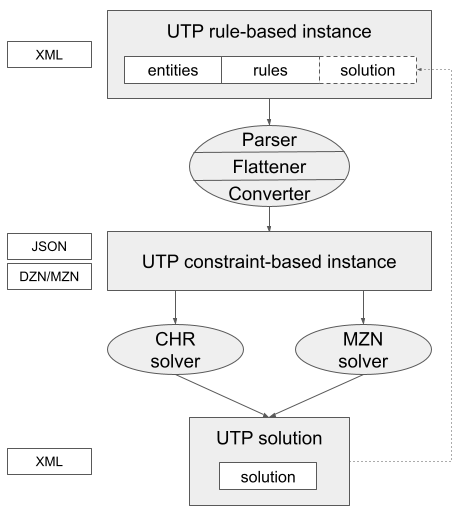
\includegraphics[scale=0.4]{img/utp_toolchain.png}
% %     \caption{The \UTP{} toolchain.}
% %     \label{fig:toolchain}
% % \end{figure}

% Note that all constraints are handled as hard constraints and each {\UTP} instance is reduced to a hard constraint satisfaction problem ({\CSP}).
% The ability to model preferences and multi-criteria objectives by the means of soft constraints is paramount in course timetabling and will be the subject of future extensions. 
% Likewise, the catalog of {\UTP} predicates still lacks important constraints (e.g., gap, distribution and pattern constraints - see e.g. \cite{2017_aizam_AIPCP,2021_chen_IEEEA}) which will be gradually added in future versions.

% \subsubsection{Data Model}
% \label{sec:entity-schema-model}
Table~\ref{table:entity-model} provides a formal specification of the schema elements.
Resources and course elements, except sessions, are referred to as \textit{entities}.
Entities are typed,
the set of sessions is cast as distinct type, 
and each type is modeled as a finite set.
% % :
% % the set of courses ${\COURSE}$, 
% % course parts ${\PART}$, 
% % classes ${\CLASS}$, 
% % teachers ${\TEACHER}$,
% % rooms ${\ROOM}$,
% % students ${\STUDENT}$, 
% % student groups ${\GROUP}$, 
% % and the domain of courses %${\COURSES}$ 
% % ${\COURSES}=\myset{\COURSE}$. 
% % ${\TYPE}$
% % (
% $
% {\TYPE}
% =
% \myset{
% {\COURSES}, 
% {\COURSE},
% {\PART},
% {\CLASS},
% {\ROOM},
% {\TEACHER},
% {\STUDENT},
% {\GROUP}
% }
% $
% % )
% denotes the set of entity types, 
% % ${\ENTITY}$
% ${\ENTITY}=\setunion{X}{\TYPE}{X}$
%  the set of entities,
% and ${\SESSION}$ the set of sessions.
The course element hierarchy
defines 1-to-many \textit{composition relations} over the pair of types
$(X,Y)$ corresponding to parent and child types
in the course element hierarchy. 
Each relation is modeled by a function ${\maptype{X}{Y}}:X\rightarrow2^{Y}$
mapping each object $i$ of type $X$
to the set ${\map{X}{Y}{i}}$ of its constitutive objects of type $Y$.
% For notational convenience, the table also represents the inverse ${\maptype{Y}{X}}:Y\rightarrow2^{X}$ of each function ${\maptype{X}{Y}}$.
% ($j\in\map{X}{Y}{i}\leftrightarrow i\in\map{Y}{X}{j}$)
For instance, 
${\maptype{\PART}{\CLASS}}$ 
models the classes of each part.
% and ${\maptype{\CLASS}{\PART}}$ 
% the (singleton) part of each class.
Each \textit{compatibility relation}
defining the allowed or assigned resources of a course element object
for a given resource type and course element type
defines a many-to-many relation
which we model the same way.
%by 2 inverse functions.
For instance, 
${\maptype{\PART}{\ROOM}}$
models the allowed rooms per part
and ${\maptype{\CLASS}{\GROUP}}$
the set of groups assigned to classes.

For notational convenience, 
the table also defines 
the maps resulting from 
the symmetric and transitive closure of the binary relation %(digraph)
merging the composition and compatibility maps.
This includes
the maps
computed over the course tree.
% \footnote{
% $\forall X,Y,Z \in {\TYPE}\cup\myset{\SESSION}:
% X\preceq^{*} Y\preceq^{*} Z 
% \Rightarrow 
% (\forall i \in X:
% \map{X}{Z}{i}=\setpartition{j}{\map{X}{Y}{i}}{\map{Y}{Z}{j}}
% $
% }
For instance, 
%function 
${\maptype{\CLASS}{\PART}}$ 
models the (singleton) part of each class,
and ${\maptype{\COURSE}{\SESSION}}$ 
the sessions of a course.
%resulting from the recursive set-union of the sessions of its parts' classes.
This also includes the 
inverse compatibility constraints
and those inherited along the course tree.
For instance, ${\maptype{\SESSION}{\ROOM}}$ models the rooms allowed for a session
which results from the composition of ${\maptype{\SESSION}{\CLASS}}$, ${\maptype{\CLASS}{\PART}}$ and ${\maptype{\PART}{\ROOM}}$.
% - 
% $
% j\in{\map{\SESSION}{\ROOM}{i}}
% \leftrightarrow 
% j\in{\map{\PART}{\ROOM}{k}}
% \wedge
% i\in{\map{\PART}{\SESSION}{k}}
% $
% )
Lastly, the table defines the constants (e.g., number of weeks),
scalar properties
(e.g., room capacity),
and remaining relations and sets (e.g. required resources, labels).
% and remaining relations (required resources) 
% and sets (labels, exclusive/inclusive sessions).

% $
% {\prec}
% =
% \myset{
% ({\COURSES},{\COURSE}),
% ({\COURSE},{\PART}),
% ({\PART},{\CLASS}),
% ({\CLASS},{\SESSION}),
% ({\TEACHER},{\PART}),
% ({\ROOM},{\PART}),
% ({\STUDENT},{\GROUP}),
% ({\GROUP},{\COURSE})
% }
% $
% denotes the relation over 
% ${\TYPE}\cup\myset{\SESSION}$ 
% that models the course hierarchy
% and the distribution of resource types over course components.

% ${\prec^{*}}$
% %${\preceq^{*}}$
% denotes the transitive %and reflexive 
% closure of
% ${\prec}$ 
% over
% ${\TYPE}\cup\myset{\SESSION}$
% and
% ${\maptype{X}{Y}}:X\rightarrow2^{Y}$
% denotes the function mapping each element of $X$ to its set of compatible elements in $Y$
% for each pair %$(X,Y)$ such that 
% %$X{\preceq^{*}}Y$.
% $X{\prec^{*}}Y$.
% For instance, 
% ${\maptype{\ROOM}{\PART}}$ 
% represents the distribution of rooms over course parts, 
% ${\maptype{\PART}{\CLASS}}$ 
% the decomposition of course parts into classes,
% ${\maptype{\CLASS}{\SESSION}}$ 
% the decomposition of classes into sessions,
% and ${\maptype{\ROOM}{\SESSION}}$ 
% the inferred distribution of rooms over sessions.
% The functions corresponding to the pairs of $\prec$
% are directly encoded in the entity model
% and the remaining functions are defined inductively using recursive aggregation. 

% We shall denote by ${\map{X}{Y}{i}}$ the image of entity $i$ of type $X$ over $2^Y$ %, i.e., the set of elements of type $Y$ compatible with $i$. 
% and by ${\maptype{Y}{X}}$ the inverse of ${\maptype{X}{Y}}$.

% Equation (\ref{model:hierarchy}) below models the hierarchical decomposition of course elements\footnote{$\disjunion$ denotes the disjoint union operation, i.e. set union over pairwise disjoint sets.},
% Equation (\ref{model:transitivity}) is the closure rule over 
% %$\preceq^{*}$. 
% $\prec^{*}$,
% %Note that each map $\maptype{\SESSION}{X}$ is the inverse of map $\maptype{X}{\SESSION}$.
% and Equation (\ref{model:inverse}) models inverse maps.

% \begin{align}
% %
% \forall (X,Y) \in 
% \myset{
% ({\COURSES},{\COURSE}),
% ({\COURSE},{\PART}),
% ({\PART},{\CLASS}),
% ({\CLASS},{\SESSION})
% }:
% Y=
% \setpartition{i}{X}{\map{X}{Y}{i}} 
% \label{model:hierarchy}
% \\
% %
% \forall X,Y,Z \in {\TYPE}\cup\myset{\SESSION}:
% X\preceq^{*} Y\preceq^{*} Z 
% \Rightarrow 
% (\forall i \in X:
% \map{X}{Z}{i}=\setpartition{j}{\map{X}{Y}{i}}{\map{Y}{Z}{j}}
% \label{model:transitivity})
% \\
% %
% \forall X,Y \in {\TYPE}:
% X\preceq^{*} Y 
% \Rightarrow 
% (\forall i \in X, j \in Y:
% j \in \map{X}{Y}{i} \Leftrightarrow i \in \map{Y}{X}{j}
% )
% \label{model:inverse}
% %\\
% %%
% %\forall X \in {\TYPE}\cup\myset{\SESSION},
% %i \in X:
% %\domarg{X}{X}{i} = \myset{i} \label{model:selfmap}
% %%
% \end{align}


%\footnote{
% The following rules apply. $\SLOT=\myset{i.\WEEKDAY.\DAILYSLOT+j.\DAILYSLOT+k\ |\ 0\leq i<\WEEK,0\leq j<\WEEKDAY,1\leq k\leq\DAILYSLOT}$.
% For each class $k$ in part $p$,
% $\myset{\sessionrank{s}\ |\ s\in\map{\CLASS}{\SESSION}{k}}=\myset{1,\ldots,\mycard{\map{\CLASS}{\SESSION}{k}}}$, 
% %$\mycard{\classparents{k}}\leq1$ 
% and $\classparents{k}\not\subset\map{\PART}{\CLASS}{p}$.
% For each pair of sessions $s,s'$, 
% $(s,s')\in\sessionranked$ iff $\map{\SESSION}{\CLASS}{s}=\map{\SESSION}{\CLASS}{s'}$ and $\sessionrank{s'}=\sessionrank{s}+1$.
% For each course part $p$,
% %$p\in\multiroomparts$ iff $\multiroompart{p}$; 
% %and 
% $\partteachermultiplicity{p}.\mycard{\map{\PART}{\SESSION}{p}}=\sum\limits_{l\in\map{\PART}{\TEACHER}{p}}{\partteacherservice{l,p}}$.}
%
%We shall denote by
%${\RANK}$
%the range of session ranks,
%${\maptype{\RANK}{\SESSION}}:\RANK\rightarrow2{^\SESSION}$
%the rank-based partitioning of sessions,
%and
%${\LABEL}$
%the set of labels 
%(${\LABEL}\subseteq2^{{\ENTITY}}$)
%completed 
%with the whole set of entities %to mock label optionality
%($\ENTITY\in{\LABEL}$)
%and singleton entities %to support identity-based selection
%($\myset{\myset{e}\ |\ e\in{\ENTITY}}\subseteq{\LABEL}$).
%As discussed in section~\ref{sec:rules},
%labels are optional filters used in rules to select entities
%hence the formal inclusion of $\ENTITY$ in ${\LABEL}$ to mock label optionality.
%Likewise, entity identifiers are used as an alternative to labels
%hence the inclusion of singleton entities in ${\LABEL}$.


\input{2-1-entity-schema-table}

% ------------------------------------------------------------
% ------------------------------------------------------------
\subsection{Solutions}
\label{sec:solution}

The solution schema is used to encode
any solution pre-computed for an instance.
%(e.g., the choice of rooms and start times for sessions).
Such a solution needs not be complete, nor consistent with the instance constraints.
An instance may hence be associated with any kind of input solution based on the
computational task,
e.g. no solution at all when generating a timetable from scratch, 
a resource allocation solution to extend into a complete timetable,
a seed solution to improve, 
or an inconsistent solution to repair.
Formally, the solution schema
supports the representation of
any decision made for a session
as to its start time,
% on time points ($\var{\SESSION}{\SLOT}{s}$),
its set of rooms
%($\var{\SESSION}{\ROOM}{s}$)
and its set of teachers.
%($\var{\SESSION}{\TEACHER}{s}$)
%for sessions.

% the 
% on time points ($\var{\SESSION}{\SLOT}{s}$),
% rooms ($\var{\SESSION}{\ROOM}{s}$)
% and lecturers ($\var{\SESSION}{\TEACHER}{s}$)
% for sessions.



%------------------------------------------------------------
%------------------------------------------------------------
\subsection{Predicates, Constraints and Rules}
\label{sec:schema-predicates-constraints-rules}

The \UTP{} schema comes with a rule language to formulate instance-specific constraints.
Rule constraints add to the built-in constraints of the schema
and all must be checked when evaluating a solution.
The rule language is designed to target groups of entities, or individual entities,
and constrain the scheduling of their sessions
from any standpoint
(e.g., an institutional rule imposing a time structure on curricula,
a disjunctive scheduling rule applied to student groups,
a rule modeling the service plan within a faculty department,
a rule for a lecturer's agenda).
%the unavailability of department staff).
% Each rule provides a compact representation
% of a conjunction of constraints on selected entities and sessions.
The schema comes with a catalog of timetabling predicates
to build rules and compile them into constraints.
It also includes a custom syntax to select
selected entities and sessions on which rules apply.
%to forge rules on selected entities and sessions.


% Both the constraint syntax and query language
All these components are designed around the concept of \textit{e-map}.
Formally, an e-map is a pair $(e_i,S_i)$ 
mapping an entity $e_i$ to a set $S_i$ of sessions.
The query language is used to forge queries that retrieve sets of e-maps.
Each query selects, filters and binds entities to sessions from instance data 
in order to extract one or more sets of e-maps.
% before assembling them into tuples.
Each rule is bound to a predicate and scoped by a query.
At flattening time, 
the query is performed to retrieve a fixed number of sets of e-maps.
The rule is then compiled into a conjunction of constraints
by computing the cross-product of the extracted sets %of e-maps
and applying the predicate to each tuple of e-maps in the cross-product.
Constraint e-maps act as guards when checking solutions
and they also narrow the scope of interpretation.
The rationale is to discard constraints that are irrelevant
(e.g., a teacher's constraint forbidding afternoon lectures while the solution only assigns him lab sessions)
and, more generally, to limit constraint checks to the proposed assignments
(e.g., checking the above lecturer's constraint on the actual lectures the solution assigns him).
% E-maps may be classified as course or resource e-maps based on their entity.

As mentioned above, 
each %\UTP{} 
constraint applies a predicate to a tuple of e-maps.
\UTP{} predicates %accept one or more e-map variable arguments.
%They 
either accept a fixed number of %have a fixed arity (the number of 
e-maps % variables % arguments)
or are variadic.
Their semantics may be indifferent to the ordering of their arguments or not,
and some accept parameters.
Besides, each predicate may be used indistinctly
with course e-maps or resource e-maps (i.e., e-maps pairing course elements or resources),
and any n-ary constraint may freely mix the two types
(e.g., a constraint booking rooms for sessions involving different classes).
Let ${\EMAP}=\ENTITY\times{2^{\SESSION}}$ denote the domain of e-maps,
% defined by
% and defined by:
% \begin{equation*}
% {\EMAP}=
% \setunion{X}{\TYPE}
% \myset{(e,S')\ |\ e\in X,
% %\emptyset\subset 
% S'\subseteq\map{X}{\SESSION}{e}}
% \end{equation*}
the general form of a %n-ary %{\UTP} 
constraint is
% \begin{equation*}
% \begin{align}
$c((e_1,S_1),\ldots,(e_n,S_n),p_1,\ldots,p_m)$ %\label{rule:constraint}
% \end{align}
% \end{equation*}
where 
$c$ is a predicate of arity $n$,
$(e_1,S_1),\ldots,(e_n,S_n)$ are e-maps ($(e_i,S_i)\in{\EMAP}$ for $i=1\ldots n$) 
and 
$p_1,\ldots,p_m$ are values for the parameters of $c$ ($m\geq0$).

The semantics of constraints relies on a join operation between constraint e-maps and solutions.
% The pairing of entities and sessions to form e-maps
% is subject to typing rules imposed by the instance schema.
% Specifically, a course element (class, part, course or course domain)
% may only be paired with some of its constitutive sessions,
% whereas a resource 
% may only be paired with some of its allowed sessions 
% (or fixed sessions in the case of students and groups).
% %consistently with the instance schema data.
% E-maps may hence be classified as course or resource e-maps.
% We associate an e-map variable to each entity of the instance
% to denote the set of sessions it is assigned in a solution.
% Course e-map variables are actually constants 
% since each one represents the fixed set of constitutive sessions of a course element.
% Resource e-map variables however do vary since sessions have to be chosen for each resource.
Note first that any solution may be cast as a tuple of e-maps 
by converting the session-to-resource assignments into resource e-maps
and re-encoding the fixed maps binding course elements to their sessions.
We say an e-map is \textit{null} if it pairs an entity with an empty set of sessions,
and, by extension, a tuple of e-maps is null if it includes a null e-map.
Given a solution and an e-map for some entity,
we call \textit{joint e-map} the pairing of the entity with the set of sessions
on which the solution and the e-map agree,
i.e., the set-intersection of the sessions of the e-map and those assigned/bound to the entity in the solution encoding.
We say a solution is \textit{inconsistent} with an e-map if their joint e-map is null.
The join operation extends to tuples by performing the operation component-wise
%By extension, %a tuple of e-maps may be joined with a solution by joining individual e-maps
and a solution is said to be inconsistent with a tuple of e-maps 
if its is inconsistent with at least one e-map in the tuple.

%As for satisfiability, 
% t
The evaluation of a solution against a constraint
%(to decide whether it is satisfied or not)
% depends on the consistency of its e-map tuple with the solution.
is conditioned by the tuple of e-maps joining those of the solution and the constraint.
If the joint tuple is null, 
the constraint is considered satisfied
(i.e., it is deemed irrelevant and discarded).
% that is, it is deemed irrelevant and hence discarded
% (e.g., a constraint forbidding afternoon lectures while the solution does not include any).
Otherwise, the predicate is evaluated on the joint e-map
and the result depends on its built-in semantics.
% \footnote{Formally, 
% a constraint 
% $c((e_1,S_1),\ldots,(e_n,S_n),p_1,\ldots,p_m)$
% is satisfied by a solution
% verifying
% $\var{X}{\SESSION}{e_i}=S'_i$ ($i=1\ldots n$)
% iff
% there exists $i\in\myset{1,\ldots,n}$ s.t. $S_i\cap S'_i=\emptyset$
% or else
% $c((e_1,S_1\cap S'_1),\ldots,(e_n,S_n\cap S'_n),p_1,\ldots,p_m))$
% holds true.}
Specifically, the predicate is assessed on
the tuple of sets obtained by substituting each set of sessions
in the joint e-map
either by the set of their assigned start times,
or the set of their assigned resources of a given type (rooms, etc).
Which type (time or resource type) to pick per e-map is fixed and predicate-specific
(e.g., a temporal predicate will substitute any e-map argument by start times).
Note that entities play no role in the evaluation %of e-map tuples
once the join and substitution operations are over:
each predicate is ultimately evaluated on sets made of start times or sets of resources.
Note also that join operations leave course e-maps unchanged unlike resource e-maps.
This means constraints applying exclusively to course e-maps are de facto unconditional. 

% course e-maps 
% E-maps bound to resources are interpreted as conditional session-to-resource assignments
% when checking constraints
% whereas e-maps defined on course elements are unconditional assignments since they model constitutive sessions.
% It follows that 
% a constraint is evaluated on every session that is mapped to a course element by one of its e-map arguments.
% Constraints that apply exclusively to course elements are therefore unconditional. 
% Note also that the use of e-maps that model the whole set of sessions compatible with an entity 
% will necessarily constrain any session that may be assigned to this entity.

The \UTP{} catalog provides predicates to cover the various dimensions of time--tabling problems.
Some only address scheduling (i.e., start times),
others room allocation, and so on.
Table~\ref{tab:predicate_catalog} and Table~\ref{tab:constraintformel} given in Appendix~\ref{appendix:constraintcatalog} describe the predicates of the catalog and provide their semantics.
%of the language
%and indicates which are variadic or parametric.
Syntactically, each rule binds a predicate to a query
and denotes the conjunction of constraints obtained 
by applying the predicate to
each tuple of e-maps extracted by the query.
% Note that a query actually retrieves one or more sets of e-maps
% and does not explicitly compute their cross product.
% Formally, a rule is a universally quantified formula 
% wherein each quantifier restricts the domain of one of the e-map variables. 
%A language of selectors is provided to build and filter domains of e-maps based on session ranks, entity identifiers, entity types, or any user-defined class of elements (e.g., team of lecturers, block of rooms). A rule hence denotes the conjunction of constraints obtained by instantiating the predicate over the cross-product of the domains of the e-map variables. 
% Let 
% ${\SELECTOR}$
% denote the language of e-map domain selectors,
% %(${\SELECTOR}\subseteq({\TYPE}\times{\LABEL}\times{2^{\RANK}})^{n}$).
A %{\UTP} 
rule has the form %is a tuple 
% \begin{align}
$c\langle{\SELECTOR},p_1,\ldots,p_m\rangle$
% $r_c(F_1,\ldots,F_m,p_1,\ldots,p_n)$
% \end{align}
and is interpreted by %The semantics of a rule $(c,D_1,\ldots,D_m,p_1,\ldots,p_n)$ is 
the %quantified 
formula
\begin{equation*}
% \begin{flalign}
\forall (e_1,S_1)\in\denote{\SELECTOR_1},\ldots,(e_n,S_n)\in\denote{\SELECTOR_{n}}: c((e_1,S_1),\ldots,(e_n,S_n),p_1,\ldots,p_m)
% \forall (e_1,S_1)\in\denote{F_1},\ldots,(e_m,S_m)\in\denote{F_{m}}: c((e_1,S_1),\ldots,(e_m,S_m),p_1,\ldots,p_n)
%&\label{rule:rule}
% \end{flalign}
\end{equation*}
where 
$c$ is a predicate of arity $n$ accepting $m$ parameters ($m\geq0$),
$\SELECTOR$ is a query sized to extract $n$ sets of e-maps,
$\denote{\SELECTOR_i}$
denotes the $i$-th set of e-maps extracted with $\SELECTOR$
 (%$F_i\in{\SELECTOR}$, 
$i=1\ldots n$),
% $
% F_i\in{\SELECTOR}
% $,
and
$p_1,\ldots p_m$ are values for the parameters of $c$.




% E-maps bound to resources are interpreted as conditional session-to-resource assignments
% when checking constraints
% whereas e-maps defined on course elements are unconditional assignments since they model constitutive sessions.
% It follows that 
% a constraint is evaluated on every session that is mapped to a course element by one of its e-map arguments.
% Constraints that apply exclusively to course elements are therefore unconditional. 

% Note also that the use of e-maps that model the whole set of sessions compatible with an entity 
% will necessarily constrain any session that may be assigned to this entity.

% In the first case, the e-map is interpreted as a set of conditional entity-to-session assignments while it is unconditional if it models a course element. 
% Specifically, a constraint is only evaluated on the sessions for which its e-map argument(s) and the considered solution propose the same entity. 
% Each predicate may be applied equally well to any type of e-map and be used to constrain resources (e.g., lecturer unavailability), course elements (e.g., class periodicity) or individual sessions (e.g., session parallelization). 
% Note that constraints on e-maps modeling sessions of course elements are de facto unconditional. 

% A rule is tied to a predicate and models a conjunction of constraints on selected classes of entities and sessions (e.g., disjunctive scheduling rule for lecturers, time constraints on the courses of a curriculum).
%For instance, unconditional start time restrictions using predicates such as {\SAMEDAILYSLOT} or {\FORBIDDENPERIOD}  may be enforced on any set of sessions bound to a course, a part, a class or more generally to the course domain. Conversely, start time restrictions on a set of sessions bound to a resource will only be enforced on those which are eventually assigned to the resource.
%Predicates serve to constrain the possible sessions of resources (e.g., unavailabilities of a teacher) or the constitutive sessions of course elements (e.g., periodicity of a class). 
%e-maps may then be adjusted to constrain candidate sessions of resources (e.g., teacher unavailability), constitutive sessions of course elements (e.g., class periodicity), or individual sessions (e.g., session sequencing and parallelization).

% All {\UTP} constraints apply to pairs, called e-maps,
% which associate an entity with a set of sessions.
% % Specifically, 
% % an e-map
% % associates a course element with a subset of its constitutive sessions,
% % or a resource with a subset of its allowed sessions.
% The domain of e-maps is denoted by ${\EMAP}$
% and defined by:
% \begin{equation*}
% {\EMAP}=
% \setunion{X}{\TYPE}
% \myset{(e,S')\ |\ e\in X,\emptyset\subset S'\subseteq\map{X}{\SESSION}{e}}
% \end{equation*}

% Constraints are built with predicates of the \UTP{} catalog.
% The signature of a predicate includes one or more e-map variables
% (i.e., variables ranging over the e-map domain),
% the number of which defines the arity of the predicate. 
% Note that some predicates may accept parameters.
% Let 
% ${\EMAP}=
% \setunion{X}{\TYPE}
% \myset{(e,S')\ |\ e\in X,S'\subseteq\map{X}{\SESSION}{e}\wedge S'\neq\emptyset}$
% denote the set of e-maps,
% The general form of a n-ary {\UTP} constraint is
% \begin{align}
% c((e_1,S_1),\ldots,(e_n,S_n),p_1,\ldots,p_k) \label{rule:constraint}
% \end{align}
% where 
% $c$ is a predicate symbol of arity $n$,
% $(e_1,S_1),\ldots,(e_n,S_n)$ are e-maps ($(e_i,S_i)\in{\EMAP}$, $i=1\ldots n$) 
% and 
% $p_1,\ldots,p_m$ are values for the parameters of $c$ ($m\geq0$).
% Formally, let $\var{E}{\SESSION}{e}$ be the variable denoting the set of sessions assigned to entity $e$ and $S'_1,\ldots,S'_m$ be sets of sessions, the conditionality of a constraint $c$ is stated as follows: 
% $(\var{E}{\SESSION}{e_1}=S'_1 \wedge\ldots\wedge\var{E}{\SESSION}{e_m}=S'_m)
% \Rightarrow
% (c((e_1,S_1),\ldots,(e_m,S_m),p_1,\ldots,p_n)
% \Leftrightarrow
% c((e_1,S_1\cap S'_1),\ldots,(e_m,S_m\cap S'_m),p_1,\ldots,p_n))$.

%Three constraints (\ref{constraint-example-1}, \ref{constraint-example-2}, \ref{constraint-example-3}) are illustrated in Figure~\ref{fig:utp-rule-1}.


% %------------------------------------------------------------
%------------------------------------------------------------
\subsection{Rules and Flattening}
\label{sec:rules-flattening}


Rules are used to state conjunctions of constraints and in particular single constraints.
Each rule is defined by a universally quantified formula which bounds the domains of the e-map variables of a given predicate.
The collection of constraints hence represented is derived by instantiating the predicate with each tuple of e-maps belonging to the cross-product of the prescribed domains.
E-map domains are not given in extension
but represented using a language of selectors
%which provides a comprehension syntax 
allowing to generate and filter e-maps.


Formally, a rule is defined by a universally quantified formula wherein quantifiers restrict the domains of the e-map variables. A language of selectors is provided to build and filter domains of e-maps based on session ranks, entity identifiers, entity types, or any user-defined class of elements (e.g., team of lecturers, block of rooms). A rule hence denotes the conjunction of constraints obtained by instantiating the predicate over the cross-product of the domains of the e-map variables. 

Let 
${\SELECTOR}$
denote the language of e-map domain selectors,
%(${\SELECTOR}\subseteq({\TYPE}\times{\LABEL}\times{2^{\RANK}})^{n}$).
a {\UTP} rule has the form %is a tuple 
\begin{align}
c(F_1,\ldots,F_m,p_1,\ldots,p_n)
\end{align}
and is interpreted by %The semantics of a rule $(c,D_1,\ldots,D_m,p_1,\ldots,p_n)$ is 
the %quantified 
formula
\begin{flalign}
&\forall (e_1,S_1)\in\denote{F_1},\ldots,(e_m,S_m)\in\denote{F_{m}}: c((e_1,S_1),\ldots,(e_m,S_m),p_1,\ldots,p_n)
&\label{rule:rule}
\end{flalign}
where 
$c$ is a predicate symbol of arity $m$,
$F_1,\ldots,F_m$ are selectors ($F_i\in{\SELECTOR}$, $i=1\ldots m$),
$\denote{F_i}$
denotes the domain of e-maps represented by
selector 
$
F_i\in{\SELECTOR}
$,
and
$p_1,\ldots p_n$ are values for the parameters of $c$ ($n\geq0$),
.

The language of selectors allows 
to target entities based on type, label or identifier
and
to filter their sets of sessions
based on session rank and mutual compatibility with other entities.
It is complete in the sense 
that it allows to construct any domain of e-maps whose entities share the same type.
For instance, one may construct the e-maps which
associate any of the rooms labeled \texttt{Building-A}
with the compatible sessions of rank 2 or 4 
that are also constitutive of course \texttt{course-1} or class \texttt{class-3}.
A selector
combines a generator and an optional list of filters.
Generators and filters are triples 
$
(T_i,L_i,O_i)
$
consisting of
an entity type
$
T_i%\in{\TYPE}
$,
an entity label or identifier
$
L_i%\in{\LABEL}
$
and
a subset of session ranks
$
O_i%\subseteq{\RANK}
$ (a.k.a., session mask),
the latter two elements being optional.
A selector 
matches any e-map
whose entity satisfies the type, label and identifier constraints of the generator
and whose %set of sessions 
image includes any compatible session
satisfying the mask of the generator
and one of the filters.
Note that rules featuring null selectors are discarded during the flattening stage. 
%Selectors are encoded as attributes in the {\XML} language
%using a syntax that borrows from the CSS selector language.
%For instance, the above example would be encoded by the following XML fragment: 
%\todo[inline]{Marc : Rajouter une phrase pour décrire brièvement la figure 3}

Let
${\RANK}$
denote the range of session ranks,
${\maptype{\RANK}{\SESSION}}:\RANK\rightarrow2{^\SESSION}$
the rank-based partitioning of sessions
($s\in\map{\RANK}{\SESSION}{o}$ iff $\sessionrank{s}=o$),
and
${\LABEL}^{*}={\LABEL}\cup\myset{\ENTITY}\cup\myset{\myset{e}\ |\ e\in{\ENTITY}}$
%${\LABEL}^{*}$
the set of labels 
%(${\LABEL}\subseteq2^{{\ENTITY}}$)
%(${\LABEL}\subseteq{\LABEL}^*$)
completed 
with the whole set of entities to mock label optionality
%($\ENTITY\in{\LABEL}^*$)
and singleton entities to support identity-based selection,
%($\myset{\myset{e}\ |\ e\in{\ENTITY}}\subseteq{\LABEL}^*$),
the language of selectors
is the set 
$
{\SELECTOR}=\cup_{n\geq1}({\TYPE}\times{\LABEL}^*\times{2^{\RANK}})^{n}
$.
%where each 
Each selector 
$
d=((T_1,L_1,O_1),\ldots,(T_k,L_k,O_k))
$
%($k\geq1$)
decomposes into a generator
$
(T_1,L_1,O_1)
$
and a possibly empty list of filters
$
((T_2,L_2,O_2),\ldots,(T_k,L_k,O_k))
$.
%A session $s$ is said to satisfy triple
%$
%(T_i,L_i,O_i)
%%\in({\TYPE}\times{\LABEL}\times{2^{\RANK}})
%$
%if
%it is compatible with
%an entity of type $T_i$ and label $L_i$ 
%($s\in\map{T_i}{\SESSION}{L_i}$)\footnote{
%%Let $X\subseteq Y$,
%$
%{\map{Y}{\SESSION}{X}}
%$
%denotes
%$
%\setunion{i}{X\cap Y}{\map{Y}{\SESSION}{i}}
%$.
%}
%and 
%if it satisfies mask $O_i$, i.e., its rank is included in $O_i$
%($s\in\map{\RANK}{\SESSION}{O_i}$).
%A selector 
%$
%d=((T_1,L_1,O_1),\ldots,(T_k,L_k,O_k))
%$
$d$ matches any e-map
whose entity has type $T_1$ and label $L_1$ and whose image includes any compatible session satisfying mask $O_1$ and any of the filters.
The set of e-maps
$\denote{d}$
matched by $d$
is defined by
%\begin{flalign*}
%\denote{d}=
%\bigcup\limits_{e\in{T_1}}
%{\myset{(e,S')
%\ |\ 
%%e\in T_1\cap L_1,
%S'=
%\map{T_1}{\SESSION}{\myset{e}\cap L_1}
%%\bigcap 
%%\map{\RANK}{\SESSION}{O_1}
%\bigcap 
%\bigcup\limits_{i=2\ldots k}
%{
%\map{T_i}{\SESSION}{L_i}
%\bigcap
%\map{\RANK}{\SESSION}{O_1\cap O_i}
%%\myset{s\in\SESSION\ |\ \sessionrank{s}\in O_1\cap O_i}
%\wedge
%S'\neq\emptyset
%}
%}
%}
%\end{flalign*}
%
%where
%$
%{\map{Y}{\SESSION}{X}}
%=
%%$
%%denotes
%%$
%\bigcup\limits_{i\in X}{\map{Y}{\SESSION}{i}}
%$
%($X\subseteq Y$)
%.
\begin{multline*}
\denote{d}=
\bigcup\limits_{e\in{T_1\cap L_1}}
\Big \{(e,S')
\ |\ 
S'=
\map{T_1}{\SESSION}{e}
\;\bigcap
%\\
\bigcup\limits_{i=2\ldots k}
{\Big(
\mape{T_i}{\SESSION}{L_i}
\bigcap
\mape{\RANK}{\SESSION}{O_1\cap O_i}
\Big)
}
\\
\wedge
S'\neq\emptyset
\Big \}
\end{multline*}

where
$
{\mape{X}{Y}{X'}}
=
%$
%denotes
%$
\bigcup\limits_{i\in X'}{\map{X}{Y}{i}}
$
with
$X'\subseteq X$
.



\todo{figure sample rules commented}
\begin{figure}[ht]
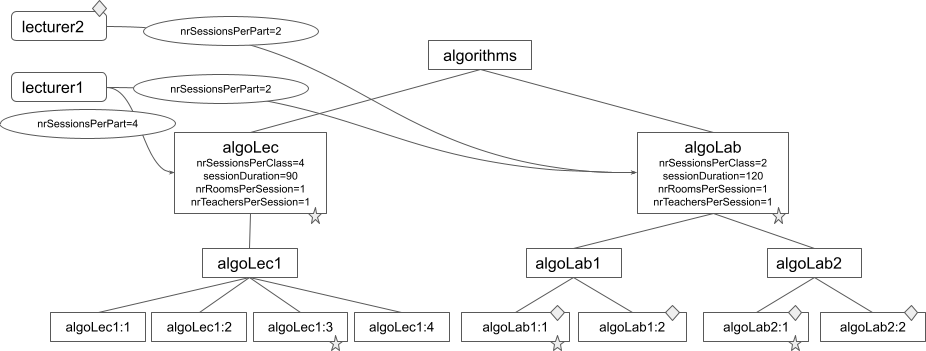
\includegraphics[scale=0.35]{img/utp_rule_1.png}


\newcounter{save_equation}
\setcounter{save_equation}{\value{equation}}
\setcounter{equation}{0}

\renewcommand{\theequation}{R\arabic{equation}}

{\footnotesize{
\begin{flalign}
&\texttt{{\FORBIDDENPERIOD}((<(\TEACHER,{lecturer2},\_)>,9120,9240)}
&\label{rule-example-1}
\\
&\texttt{{\SEQUENCED}(<(\CLASS,\_,\myset{3}),(\PART,{algoLec},\_)>,
<(\CLASS,\_,\myset{1}),(\PART,{algoLab},\_)>)}
&\label{rule-example-2}
\end{flalign}
}}


\setcounter{equation}{0}
\renewcommand{\theequation}{C\arabic{equation}}

%
{
\footnotesize
\begin{flalign}
\nonumber &\texttt{{\FORBIDDENPERIOD}((lecturer2,\{algoLab1:1,algoLab1:2,algoLab2:1,algoLab2:2\}),}\\
 & \texttt{9120,9240)}
&\label{constraint-example-1}
\\
&\texttt{{\SEQUENCED}((algoLec1,\{algoLec1:3\}), (algoLab1,\{algoLab1:1\}))}
&\label{constraint-example-2}
\\
&\texttt{{\SEQUENCED}((algoLec1,\{algoLec1:3\}), (algoLab2,\{algoLab2:1\})}
&\label{constraint-example-3}
\end{flalign}
}
%

\caption{Rules flattening and corresponding constraints on a toy example.}
\label{fig:utp-rule-1}

\setcounter{equation}{\value{save_equation}}
\end{figure}


Figure~\ref{fig:utp-rule-1} illustrates the rules flattening process on a toy example.
Course \texttt{algorithms} is split into a lecture part \texttt{algoLec} and a lab part \texttt{algoLab}.
The lecture part has a single class of 4 sessions taught by \texttt{lecturer1} and the lab part has 2 classes of 2 sessions each taught by \texttt{lecturer1} or \texttt{lecturer2}.
%Figure~\ref{fig:utp-rule-1} illustrates the flattening of the following rules: 
%on a simple model consisting of 2 teachers and & course subdivided into 2 parts, 3 classes and 8 sessions. The first rule forbids a time period for 
Rule~\ref{rule-example-1} %below
requires that \texttt{lecturer2} has no session between slots $9120$ and $9240$, corresponding for instance to 8am and 10am on Tuesday of week 2. % assuming a granularity of 1 minute per time slot. 
%In this rule, $9120$ (resp. $9240$) is the value\footnote{Each possible session schedule is mapped to a single value. All possible values make up the domain of a session.} that corresponds to 8am on Tuesday (resp. 10am on Tuesday) of week 2. 
The selector includes no mask and no filter hence matches with all possible sessions of \texttt{lecturer2} 
as indicated with diamonds on Figure~\ref{fig:utp-rule-1}. 
The resulting domain of e-maps is the singleton $\myset{(lecturer2,\map{\TEACHER}{\SESSION}{lecturer2})}$
and the rule is flattened into a single \texttt{\FORBIDDENPERIOD} constraint (\ref{constraint-example-1}). %$\myset{\map{\TEACHER}{\SESSION}{teacher2}}$.
Rule~\ref{rule-example-2}
%requires that the first practical session in Algorithmic \todo[inline]{Marc : pourquoi algo ?} start after the third lecture.
requires that the first sessions of the labs start after the third lecture.
The two selectors include a filter. The first selector matches with all class sessions of rank 3 in part \texttt{algoLec}, 
and the second matches with all class sessions of rank 1 in part \texttt{algoLab} as indicated with stars on the figure.
The rule is flattened into 2 \texttt{\SEQUENCED} constraints (\ref{constraint-example-2} and \ref{constraint-example-3}) corresponding to the cross product of the e-map domains 
%$\myset{(algoLec1,\map{\RANK}{\SESSION}{3}\cap\map{\PART}{\SESSION}{algoLec})}$
%and $\myset{(algoPra1,\map{\RANK}{\SESSION}{1}\cap\map{\PART}{\SESSION}{algoPra}),(algoPra2,\map{\RANK}{\SESSION}{1}\cap\map{\PART}{\SESSION}{algoPra})}$.
$\myset{(algoLec1,\myset{s\in\SESSION\ |\ \sessionrank{s}=3}\cap\map{\PART}{\SESSION}{algoLec})}$
and $\myset{(algoLab1,\myset{s\in\SESSION\ |\ \sessionrank{s}=1}\cap\map{\PART}{\SESSION}{algoLab}),(algoLab2,\myset{s\in\SESSION\ |\ \sessionrank{s}=1}\cap\map{\PART}{\SESSION}{algoLab})}$.
\coco{Core constraint }

% \input{2-1-1-variables-table}
% \input{2-1-1-core-constraints-table}
% The constraint~\ref{ctr:allowedslots} restricts the set of possible values to the allocated starting slots in the corresponding course part for a session. Similarly, constraint~\ref{ctr:allowedrooms} limits the set of possible values to the allocated rooms in the corresponding course part for a session. Likewise, for teachers, constraint~\ref{ctr:allowedteachers} restricts the set of possible teachers.

% To express the desired number of rooms per course session, we refer to cardinality constraint~\ref{ctr:cardinalmultiroom}, while for teachers, we reference constraint~\ref{ctr:cardinalmultiteacher}. Constraint~\ref{ctr:cumulativeroomcapacity} specifies that each session must take place in a set of rooms whose cumulative capacity can accommodate the groups enrollment of the session.

% More generally, constraint~\ref{ctr:roomuse} prohibits the cumulative capacity of sessions taking place in a room, for a given time slot, don't exceeding the room's capacity. Constraint~\ref{ctr:nooverlap2days} ensures that no session spans across two different days. 
% %Note that sessions are considered uninterruptible and, in particular, may not overlap two days. 
% Finally, constraint~\ref{ctr:coresumvariables} establishes the relationship between auxiliary time values and the starting slot variable for each session.

% For each teacher is allocated a fixed number of sessions in each course part he is eligible for, leaving lecturer-to-session assignment decisions to solvers (\hyperref[feat:service]{``service''}) and we used the constraint required\_teacher to explain this relation. And symmetrically, each room allowed to %
% %in a course part may be freely allocated to any session of the part (possibly none \hyperref[feat:roommodal]{``no room''}) but 
% the model provides the flexibility to mark a room as mandatory (e.g., requiredRooms constraint) in which case it will host or co-host all the sessions\hyperref[feat:ressourcedistribution]{``ressource distribution''}. 



\section{A Feature Model}
\label{sec:feature-model}
This section introduces a feature model
for educational timetabling problems
based on the \UTP{} schema.
The model is not meant to be exhaustive, nor stable,
but is a first attempt
to capture %key 
the key variability points  (the features)
in the family of instances
that can be expressed with the schema.
%, effectively decomposing the problem space into different classes.
%expressible in the \UTP{} schema.
Some features are plain flags characterizing the compliance of an instance to the schema (e.g., whether courses are hierarchically structured or not)
while others are logical assertions on instance data (e.g., whether the number of weeks is set to 1 or not).
% or by a textual description of a schema-level constraint .
% a logical statement that is based on instance data (e.g., )
In either case, each feature may be checked against any instance
and, in turn, instances classified into different classes
based on the features they satisfy.

The feature model hence decomposes the space of \UTP{} problems
which serves different purposes.
One is to quickly assess whether 
the schema 
is applicable to %model and tackle 
a particular setting. % an instance wherever it comes from.
Another is to provide a straightforward characterization of problem classes,
similarly to the way 3-field notation is used in other scheduling domains \cite{1979_graham_ADM,robinX_3field,scheduling_zoo}.%ajouter robinX ? et schduling zoo ?  
The aim is also to facilitate the comparison of \UTP{} with competing schemas, %for timetabling problems,
possibly paving the way for formal reductions between problems
and conversions between schemas.
% Beyond instance classification, 
Lastly, the feature model can guide the configuration of efficient computational models
by using features to reformulate or optimize %or reformulate 
built-in constraints and predicate implementations.
% We first provide background on feature modeling then discuss \UTP{} features and their structuring.

% ~~%%tableau des features
%\colorbox{gray}{\strut Votre texte ici}
% \newcommand{\medcirc}{\text{\raisebox{0.25ex}{\large$\circ$}}}
% \newcommand{\medbullet}{\text{\raisebox{0.25ex}{\large$\bullet$}}}%command possible

\begin{table}[!ht]
    \centering
    \arrayrulecolor{black}
    \begin{tabular}{|c|c|l|c|l|}
    %\begin{tabular}{cclcl}
        
        \hline
        % nom &&&&&\\
        \multirow{3}{*}{$\medbullet$}& \multirow{3}*{\rotatebox{90}{\hspace{-2pt}\courses\label{featmodel:courses}}} &\multirow{3}*{$\medcirc$}&  \cellcolor[gray]{.9} &\cellcolor[gray]{.9}\\
        && &\multirow{-2}*{\cellcolor[gray]{.9}\coursehierarchy~\label{featmodel:hierarchy}} &\multirow{-2}*{\cellcolor[gray]{.9} \textit{courses are decomposed hierarchically into sessions}}\\
        % \cellcolor[gray]{.9}course-hierarchy~\label{featmodel:hierarchy} & \multirow{2}*{*}&\cellcolor[gray]{.9} $\exists\; \map{\ENTITY}{\ENTITY}{x}$\\
         &&& \event~\label{featmodel:event} & ~\textit{events unrelated to courses must be scheduled}\\%des réunions pas student
         % event~\label{featmodel:event} &&$\exists p\in\PART \;:\;\multiroompartmax{p} = 0 \vee \partteachermultiplicitymax{p} = 0 \vee |\map{\PART}{\GROUP}{p}| = \emptyset  $ \\%des réunions pas student        
        \hline

        %horizon &&&&\\
       \multirow{3}{*}{$\medbullet$}& \multirow{3}*{\rotatebox{90}{\hspace{-2pt}\timing\label{featmodel:timing}}} &\multirow{3}*{$\medcirc$} &\cellcolor[gray]{.9}\fullperiod~\label{featmodel:fullperiod} &\cellcolor[gray]{.9} \textit{weeks are consecutive calendar weeks}\\
        % \cellcolor[gray]{.9}full-period~\label{featmodel:fullperiod} &\multirow{3}*{*}&\cellcolor[gray]{.9} |real\_week(max(W)) - real\_week(min(W))| = w-1\\
        &&& \fullweek~\label{featmodel:fullweek} & $\;d= 7$\\
        &&& \cellcolor[gray]{.9}\singleweek~\label{featmodel:singleweek} & \cellcolor[gray]{.9}$\;w = 1$\\
        \hline%timing
        
%        \multicolumn{3}{|c|}{\scheduling}\\ 
        \multirow{5}{*}{$\medbullet$} & \multirow{5}*{\rotatebox{90}{\hspace{-2pt}\scheduling}} &\multirow{5}*{$\medcirc$}&  &
        $\forall s_i,s_j\in\SESSION,s_i\neq s_j,\forall h_i \in \partallowedslots{s_i},\forall h_j\in\partallowedslots{s_j}\:\  $\\
        &&& \multirow{-2}*{\nooverlap~\label{featmodel:nooverlap}}&$\;h_i<h_j \land h_i \div \dailyslot = h_j \div \dailyslot:\;h_i+\sessionduration{s_i} \leq h_j$\\
        % \cellcolor[gray]{.9}no-overlap~\label{featmodel:nooverlap} &\multirow{5}*{*}&\cellcolor[gray]{.9} $\forall s_i,s_j\in S,s_i\neq s_j,\forall k \in 1..|M_i|,l\in1..|M_j|\ s.t.\ M_{i,k}<M_{j,l}:$\\
        % &&$M_{i,k}+\sessionduration{s_i} \leq M_{j,l}$\\
         %\cellcolor[gray]{.9}
         &&& \cellcolor[gray]{.9}\sameduration~\label{featmodel:sameduration} & \cellcolor[gray]{.9}%\cellcolor[gray]{.9}
         $\;\forall s_i,s_i \in \SESSION, \sessionduration{s_i} = \sessionduration{s_i}$ \\
         
       % &&& \cellcolor[gray]{.9} &\cellcolor[gray]{.9}$\;\alpha = gcd(M_{i,k} - M_{j,l} \mid i,j \in \SESSION, k \in \map{\SESSION}{\SLOT}{i}, l \in \map{\SESSION}{\SLOT}{j})$\\
       % 
       % &&& \multirow{-2}*{\cellcolor[gray]{.9}\synchronous}~\label{featmodel:synchronous}&\cellcolor[gray]{.9}$\;\land \alpha = \min(M_{i,k} - M_{j,l} \mid  i,j \in \SESSION, k \in \map{\SESSION}{\SLOT}{i}, l \in \map{\SESSION}{\SLOT}{j})$\\
         
         &&&&~Let $A=\{h_j-h_i\mid s_i,s_j\in\SESSION,h_i\in\map{\SESSION}{\SLOT}{s_i}, h_j\in\map{\SESSION}{\SLOT}{s_j},$\\
         
         &&&\multirow{-2}*{\synchronous}~\label{featmodel:synchronous}&$\; s_i\ne s_j,\;h_i<h_j\}: gcd(A) = \min(A) \land gcd(A)>1$\\ 
        \hline

%        %hosting
        \multirow{7}{*}{$\medcirc$}&\multirow{7}*{\rotatebox{90}{\hspace{-2pt}\hosting\label{featmodel:hosting}}}&\multirow{3}*{+}& \cellcolor[gray]{.9}\noroom~\label{featmodel:noroom} & \cellcolor[gray]{.9} $\exists p \in \PART,\;\multiroompartmin{p}=\multiroompartmax{p} = 0 $\\
         &&& \singleroom~\label{featmodel:singleroom} &$\;\exists p \in \PART,\;\multiroompartmin{p}=\multiroompartmax{p} = 1\;$\\
       &&& \cellcolor[gray]{.9}\multiroom~\label{featmodel:multiroom} &\cellcolor[gray]{.9} $\exists p \in \PART,\;\multiroompartmin{p}\geq1 \land \multiroompartmax{p} > 1\;$
         \\[-0.75em]
         \arrayrulecolor{black}
              &&\multicolumn{3}{c|}{\tikz{\draw[dashed, line width=0.4pt, yshift=-0.5\arrayrulewidth] (0,0) -- (\linewidth,0);}} \\[-0.58ex]
        %\\
       %\nfois{2}{3}
        &&$\medcirc$& \roomcapacityfeat~\label{featmodel:roomcapacity} & $\;\forall r \in \ROOM,\; \roomcapacity{r} \neq  \emptyset$
        %\cline{3-5}
        \\[-0.75em]
        \arrayrulecolor{black}
             &&\multicolumn{3}{c|}{\tikz{\draw[dashed, line width=0.4pt, yshift=-0.5\arrayrulewidth] (0,0) -- (\linewidth,0);}} \\[-0.58ex]
       & &\multirow{3}*{1} & \cellcolor[gray]{.9}\allexclusive~\label{featmodel:allexclusive}&\cellcolor[gray]{.9} $ \SESSIONEX = \SESSION $
       \\%[0.4em]
       
      & &  &\noneexclusive~\label{featmodel:noneexclusive}  &$\;\SESSIONINC = \SESSION $ \textit{(Not compatible with ``multi-room'')}\\
       && &\cellcolor[gray]{.9}\someexclusive~\label{featmodel:someexclusive} & \cellcolor[gray]{.9} $ \SESSIONEX \ne \emptyset \land   \SESSIONINC \ne \emptyset$ %\; \SESSIONINC \disjunion  \SESSIONEX  = \SESSION $
        \\
        \hline  
        \multirow{5}{*}{$\medcirc$} & \multirow{5}*{\rotatebox{90}{\hspace{-2pt}\teaching\label{featmodel:teaching}}} & \multirow{3}*{+}&\noteacher~\label{featmodel:noteacher} &$\;\exists p \in \PART,\;\partteachermultiplicitymin{p}=\partteachermultiplicitymax{p} = 0 $\\
      &&& \cellcolor[gray]{.9}\singleteacher~\label{featmodel:singleteacher}& \cellcolor[gray]{.9}$\;\exists p \in \PART,\;\partteachermultiplicitymin{p}=\partteachermultiplicitymax{p} = 1 $\\
       &&& \multiteacher~\label{featmodel:multiteacher} &$\;\exists p \in \PART,\;\partteachermultiplicitymin{p}\geq1\land\partteachermultiplicitymax{p} >1 $%\\
        \\[-0.75em]
        \arrayrulecolor{black}
        &&\multicolumn{3}{c|}{\tikz{\draw[dashed, line width=0.4pt, yshift=-0.5\arrayrulewidth] (0,0) -- (\linewidth,0);}} \\[-0.58ex]

       &&\multirow{2}*{$\medcirc$}& \cellcolor[gray]{.9}\teacheroverlap~\label{featmodel:teacheroverlap} &\cellcolor[gray]{.9}$\;\forall t \in\TEACHER,\forall s_i,s_j \in \map{\TEACHER}{\SESSION}{t},s_i+\sessionduration{s_i} \leq s_j \vee s_i \geq s_j +\sessionduration{s_j}$ \\
%       & & &&$\;s_i \geq s_j +\sessionduration{s_j}$ \\
       &&& \service~\label{featmodel:service}&~\textit{service constraints apply to teachers}\\ %
       % \multirow{-2}*{\cellcolor[gray]{.9}service~\label{featmodel:service}}&&\cellcolor[gray]{.9}}$\;\land \sum\limits_{t \in \map{\TEACHER}{\SESSION}{p}} n_{p,t} \geq \map{\PART}{\SESSION}{p} $\\ %(\sum\limits_{\forall s \in \SESSION} (t \in \var{\SESSION}{\TEACHER}{s})) = n $\\
       % \cellcolor[gray]{.9}&&\cellcolor[gray]{.9}}$\;\exists p \in \PART,\forall t \in \map{\PART}{\TEACHER}{p},\;\forall p \in \PART,\;\uexists n_{p,t} \in \mathbb{N},\; n_{p,t} \geq 0 \land n_{p,t} \leq |\map{\PART}{\SESSION}{p}|$\\
       % \multirow{-2}*{\cellcolor[gray]{.9}service~\label{featmodel:service}}&&\cellcolor[gray]{.9}}$\;\land \sum\limits_{t \in \map{\TEACHER}{\SESSION}{p}} n_{p,t} \geq \map{\PART}{\SESSION}{p} $\\
        \hline

        
       \multirow{4}{*}{$\medbullet$} & \multirow{4}*{\rotatebox{90}{\hspace{-2pt}\attending}}&\multirow{4}*{$\medcirc$}& \cellcolor[gray]{.9}  & \cellcolor[gray]{.9}$\;\forall g \in\GROUP,\forall s_i,s_j \in \map{\GROUP}{\SESSION}{g}, s_i+\sessionduration{s_i} \leq s_j \vee $ \\
         & &&\cellcolor[gray]{.9}\multirow{-2}*{\studentoverlap~\label{featmodel:groupoverlap}} & \cellcolor[gray]{.9}$\;s_i \geq s_j +\sessionduration{s_j} $ \\
          %TODO
         &&& \multirow{2}*{\sectioning~\label{featmodel:sectioning}} &~\textit{student groups must be fixed and pre-assigned}\\
         && & &~\textit{to classes}\\
          % group~\label{featmodel:group}& &$\;\forall g \in \GROUP,\;\exists \STUDENT' \subseteq\STUDENT ,\;\forall u\in \STUDENT',group(u) = g $ \\
        \hline
       % & day off student& \checkmark & \checkmark & & & \\

        \multirow{6}{*}{$\medcirc$}&\multirow{6}*{\rotatebox{90}{\hspace{-2pt}\aspects\label{featmodel:aspects}}}&\multirow{6}*{$\medcirc$} &  \cellcolor[gray]{.9}\availability & \cellcolor[gray]{.9} \textit{\ALLOWEDSLOTS, \FORBIDDENSLOTS, \ALLOWEDGRIDS,\ ...}\\%day off teacher
        
        &&& \periodicity & ~\textit{\PERIODIC, \ALLOWEDGRIDS,\SAMEROOMS, \DIFFERENTTEACHERS,\ ...} \\

         
       & & & \cellcolor[gray]{.9}\sessiondistribution & \cellcolor[gray]{.9} \textit{\SAMESLOT, \DIFFERENTDAY, \SEQUENCED, \NOOVERLAP}\\
        
      & && \travel & ~\textit{\COMPACTNESS, \GAP,\ ...}\\

     &&& \cellcolor[gray]{.9}\adjacency &\cellcolor[gray]{.9} \textit{\SAMEROOMS, \ADJACENTROOMS, \DIFFERENTTEACHERS,\ ...} \\

       &&& \resourcedistribution&  ~\textit{\ALLOWEDROOMS, \REQUIREDTEACHERS,\ ...} \\
       % &&& &\multicolumn{1}{l|}{%\hspace{2.55em}
       %   ~\textit{required\_rooms} }  \\%%distribution des profs & room
       % % & lunch time& & \checkmark & & \checkmark & \\% event
        \hline

    \end{tabular}
    \caption{A feature model for \UTP{}.}
    \label{tab:features}
    
\end{table} 

%%%%%%%%%%%%%%%%%%%%%%%%%%%%%%%%%%%%%%%%%%%%%%%%%%%%%%%%
% \subsubsection{Feature Modelling}
% \label{sec:feature-modelling}
We first recall the basic
%terminology,
notations 
and definitions commonly used in feature modeling languages \cite{1990_kang_TR,2002_czarnecki_ECOOP,2019_damir_ACM}.
A feature model is a tree-like structure connecting features
and factoring in different feature configurations.
A %feature 
configuration is a subset of features
selected from %a feature 
the model.
The configuration process is subject to constraints 
that primarily capture dependencies that 
exist between a feature and its children (a.k.a., sub-features). 
These fall into 4 categories:
\textit{mandatory sub-feature} (it must be selected if the parent is) labeled by $\medbullet$,
\textit{optional sub-feature} (it may be selected if the parent is) labeled by $\medcirc$,
\textit{or-feature} (at least one of the sub-features must be selected) labeled by $+$, 
and \textit{xor-feature} (exactly one sub-feature must be selected) labeled by $1$.
Finer-grained cardinality constraints may apply
as well as cross-tree constraints modeling dependencies or incompatibilities 
between features that sit in different branches.
% A feature model is readily viewable with a feature diagram
% annotating features and parent subfeatures.

%%%%%%%%%%%%%%%%%%%%%%%%%%%%%%%%%%%%%%%%%%%%%%%%%%%%%%%%
% \subsubsection{Feature Model}
% \label{sec:feature-model}
~~%%tableau des features
%\colorbox{gray}{\strut Votre texte ici}
% \newcommand{\medcirc}{\text{\raisebox{0.25ex}{\large$\circ$}}}
% \newcommand{\medbullet}{\text{\raisebox{0.25ex}{\large$\bullet$}}}%command possible

\begin{table}[!ht]
    \centering
    \arrayrulecolor{black}
    \begin{tabular}{|c|c|l|c|l|}
    %\begin{tabular}{cclcl}
        
        \hline
        % nom &&&&&\\
        \multirow{3}{*}{$\medbullet$}& \multirow{3}*{\rotatebox{90}{\hspace{-2pt}\courses\label{featmodel:courses}}} &\multirow{3}*{$\medcirc$}&  \cellcolor[gray]{.9} &\cellcolor[gray]{.9}\\
        && &\multirow{-2}*{\cellcolor[gray]{.9}\coursehierarchy~\label{featmodel:hierarchy}} &\multirow{-2}*{\cellcolor[gray]{.9} \textit{courses are decomposed hierarchically into sessions}}\\
        % \cellcolor[gray]{.9}course-hierarchy~\label{featmodel:hierarchy} & \multirow{2}*{*}&\cellcolor[gray]{.9} $\exists\; \map{\ENTITY}{\ENTITY}{x}$\\
         &&& \event~\label{featmodel:event} & ~\textit{events unrelated to courses must be scheduled}\\%des réunions pas student
         % event~\label{featmodel:event} &&$\exists p\in\PART \;:\;\multiroompartmax{p} = 0 \vee \partteachermultiplicitymax{p} = 0 \vee |\map{\PART}{\GROUP}{p}| = \emptyset  $ \\%des réunions pas student        
        \hline

        %horizon &&&&\\
       \multirow{3}{*}{$\medbullet$}& \multirow{3}*{\rotatebox{90}{\hspace{-2pt}\timing\label{featmodel:timing}}} &\multirow{3}*{$\medcirc$} &\cellcolor[gray]{.9}\fullperiod~\label{featmodel:fullperiod} &\cellcolor[gray]{.9} \textit{weeks are consecutive calendar weeks}\\
        % \cellcolor[gray]{.9}full-period~\label{featmodel:fullperiod} &\multirow{3}*{*}&\cellcolor[gray]{.9} |real\_week(max(W)) - real\_week(min(W))| = w-1\\
        &&& \fullweek~\label{featmodel:fullweek} & $\;d= 7$\\
        &&& \cellcolor[gray]{.9}\singleweek~\label{featmodel:singleweek} & \cellcolor[gray]{.9}$\;w = 1$\\
        \hline%timing
        
%        \multicolumn{3}{|c|}{\scheduling}\\ 
        \multirow{5}{*}{$\medbullet$} & \multirow{5}*{\rotatebox{90}{\hspace{-2pt}\scheduling}} &\multirow{5}*{$\medcirc$}&  &
        $\forall s_i,s_j\in\SESSION,s_i\neq s_j,\forall h_i \in \partallowedslots{s_i},\forall h_j\in\partallowedslots{s_j}\:\  $\\
        &&& \multirow{-2}*{\nooverlap~\label{featmodel:nooverlap}}&$\;h_i<h_j \land h_i \div \dailyslot = h_j \div \dailyslot:\;h_i+\sessionduration{s_i} \leq h_j$\\
        % \cellcolor[gray]{.9}no-overlap~\label{featmodel:nooverlap} &\multirow{5}*{*}&\cellcolor[gray]{.9} $\forall s_i,s_j\in S,s_i\neq s_j,\forall k \in 1..|M_i|,l\in1..|M_j|\ s.t.\ M_{i,k}<M_{j,l}:$\\
        % &&$M_{i,k}+\sessionduration{s_i} \leq M_{j,l}$\\
         %\cellcolor[gray]{.9}
         &&& \cellcolor[gray]{.9}\sameduration~\label{featmodel:sameduration} & \cellcolor[gray]{.9}%\cellcolor[gray]{.9}
         $\;\forall s_i,s_i \in \SESSION, \sessionduration{s_i} = \sessionduration{s_i}$ \\
         
       % &&& \cellcolor[gray]{.9} &\cellcolor[gray]{.9}$\;\alpha = gcd(M_{i,k} - M_{j,l} \mid i,j \in \SESSION, k \in \map{\SESSION}{\SLOT}{i}, l \in \map{\SESSION}{\SLOT}{j})$\\
       % 
       % &&& \multirow{-2}*{\cellcolor[gray]{.9}\synchronous}~\label{featmodel:synchronous}&\cellcolor[gray]{.9}$\;\land \alpha = \min(M_{i,k} - M_{j,l} \mid  i,j \in \SESSION, k \in \map{\SESSION}{\SLOT}{i}, l \in \map{\SESSION}{\SLOT}{j})$\\
         
         &&&&~Let $A=\{h_j-h_i\mid s_i,s_j\in\SESSION,h_i\in\map{\SESSION}{\SLOT}{s_i}, h_j\in\map{\SESSION}{\SLOT}{s_j},$\\
         
         &&&\multirow{-2}*{\synchronous}~\label{featmodel:synchronous}&$\; s_i\ne s_j,\;h_i<h_j\}: gcd(A) = \min(A) \land gcd(A)>1$\\ 
        \hline

%        %hosting
        \multirow{7}{*}{$\medcirc$}&\multirow{7}*{\rotatebox{90}{\hspace{-2pt}\hosting\label{featmodel:hosting}}}&\multirow{3}*{+}& \cellcolor[gray]{.9}\noroom~\label{featmodel:noroom} & \cellcolor[gray]{.9} $\exists p \in \PART,\;\multiroompartmin{p}=\multiroompartmax{p} = 0 $\\
         &&& \singleroom~\label{featmodel:singleroom} &$\;\exists p \in \PART,\;\multiroompartmin{p}=\multiroompartmax{p} = 1\;$\\
       &&& \cellcolor[gray]{.9}\multiroom~\label{featmodel:multiroom} &\cellcolor[gray]{.9} $\exists p \in \PART,\;\multiroompartmin{p}\geq1 \land \multiroompartmax{p} > 1\;$
         \\[-0.75em]
         \arrayrulecolor{black}
              &&\multicolumn{3}{c|}{\tikz{\draw[dashed, line width=0.4pt, yshift=-0.5\arrayrulewidth] (0,0) -- (\linewidth,0);}} \\[-0.58ex]
        %\\
       %\nfois{2}{3}
        &&$\medcirc$& \roomcapacityfeat~\label{featmodel:roomcapacity} & $\;\forall r \in \ROOM,\; \roomcapacity{r} \neq  \emptyset$
        %\cline{3-5}
        \\[-0.75em]
        \arrayrulecolor{black}
             &&\multicolumn{3}{c|}{\tikz{\draw[dashed, line width=0.4pt, yshift=-0.5\arrayrulewidth] (0,0) -- (\linewidth,0);}} \\[-0.58ex]
       & &\multirow{3}*{1} & \cellcolor[gray]{.9}\allexclusive~\label{featmodel:allexclusive}&\cellcolor[gray]{.9} $ \SESSIONEX = \SESSION $
       \\%[0.4em]
       
      & &  &\noneexclusive~\label{featmodel:noneexclusive}  &$\;\SESSIONINC = \SESSION $ \textit{(Not compatible with ``multi-room'')}\\
       && &\cellcolor[gray]{.9}\someexclusive~\label{featmodel:someexclusive} & \cellcolor[gray]{.9} $ \SESSIONEX \ne \emptyset \land   \SESSIONINC \ne \emptyset$ %\; \SESSIONINC \disjunion  \SESSIONEX  = \SESSION $
        \\
        \hline  
        \multirow{5}{*}{$\medcirc$} & \multirow{5}*{\rotatebox{90}{\hspace{-2pt}\teaching\label{featmodel:teaching}}} & \multirow{3}*{+}&\noteacher~\label{featmodel:noteacher} &$\;\exists p \in \PART,\;\partteachermultiplicitymin{p}=\partteachermultiplicitymax{p} = 0 $\\
      &&& \cellcolor[gray]{.9}\singleteacher~\label{featmodel:singleteacher}& \cellcolor[gray]{.9}$\;\exists p \in \PART,\;\partteachermultiplicitymin{p}=\partteachermultiplicitymax{p} = 1 $\\
       &&& \multiteacher~\label{featmodel:multiteacher} &$\;\exists p \in \PART,\;\partteachermultiplicitymin{p}\geq1\land\partteachermultiplicitymax{p} >1 $%\\
        \\[-0.75em]
        \arrayrulecolor{black}
        &&\multicolumn{3}{c|}{\tikz{\draw[dashed, line width=0.4pt, yshift=-0.5\arrayrulewidth] (0,0) -- (\linewidth,0);}} \\[-0.58ex]

       &&\multirow{2}*{$\medcirc$}& \cellcolor[gray]{.9}\teacheroverlap~\label{featmodel:teacheroverlap} &\cellcolor[gray]{.9}$\;\forall t \in\TEACHER,\forall s_i,s_j \in \map{\TEACHER}{\SESSION}{t},s_i+\sessionduration{s_i} \leq s_j \vee s_i \geq s_j +\sessionduration{s_j}$ \\
%       & & &&$\;s_i \geq s_j +\sessionduration{s_j}$ \\
       &&& \service~\label{featmodel:service}&~\textit{service constraints apply to teachers}\\ %
       % \multirow{-2}*{\cellcolor[gray]{.9}service~\label{featmodel:service}}&&\cellcolor[gray]{.9}}$\;\land \sum\limits_{t \in \map{\TEACHER}{\SESSION}{p}} n_{p,t} \geq \map{\PART}{\SESSION}{p} $\\ %(\sum\limits_{\forall s \in \SESSION} (t \in \var{\SESSION}{\TEACHER}{s})) = n $\\
       % \cellcolor[gray]{.9}&&\cellcolor[gray]{.9}}$\;\exists p \in \PART,\forall t \in \map{\PART}{\TEACHER}{p},\;\forall p \in \PART,\;\uexists n_{p,t} \in \mathbb{N},\; n_{p,t} \geq 0 \land n_{p,t} \leq |\map{\PART}{\SESSION}{p}|$\\
       % \multirow{-2}*{\cellcolor[gray]{.9}service~\label{featmodel:service}}&&\cellcolor[gray]{.9}}$\;\land \sum\limits_{t \in \map{\TEACHER}{\SESSION}{p}} n_{p,t} \geq \map{\PART}{\SESSION}{p} $\\
        \hline

        
       \multirow{4}{*}{$\medbullet$} & \multirow{4}*{\rotatebox{90}{\hspace{-2pt}\attending}}&\multirow{4}*{$\medcirc$}& \cellcolor[gray]{.9}  & \cellcolor[gray]{.9}$\;\forall g \in\GROUP,\forall s_i,s_j \in \map{\GROUP}{\SESSION}{g}, s_i+\sessionduration{s_i} \leq s_j \vee $ \\
         & &&\cellcolor[gray]{.9}\multirow{-2}*{\studentoverlap~\label{featmodel:groupoverlap}} & \cellcolor[gray]{.9}$\;s_i \geq s_j +\sessionduration{s_j} $ \\
          %TODO
         &&& \multirow{2}*{\sectioning~\label{featmodel:sectioning}} &~\textit{student groups must be fixed and pre-assigned}\\
         && & &~\textit{to classes}\\
          % group~\label{featmodel:group}& &$\;\forall g \in \GROUP,\;\exists \STUDENT' \subseteq\STUDENT ,\;\forall u\in \STUDENT',group(u) = g $ \\
        \hline
       % & day off student& \checkmark & \checkmark & & & \\

        \multirow{6}{*}{$\medcirc$}&\multirow{6}*{\rotatebox{90}{\hspace{-2pt}\aspects\label{featmodel:aspects}}}&\multirow{6}*{$\medcirc$} &  \cellcolor[gray]{.9}\availability & \cellcolor[gray]{.9} \textit{\ALLOWEDSLOTS, \FORBIDDENSLOTS, \ALLOWEDGRIDS,\ ...}\\%day off teacher
        
        &&& \periodicity & ~\textit{\PERIODIC, \ALLOWEDGRIDS,\SAMEROOMS, \DIFFERENTTEACHERS,\ ...} \\

         
       & & & \cellcolor[gray]{.9}\sessiondistribution & \cellcolor[gray]{.9} \textit{\SAMESLOT, \DIFFERENTDAY, \SEQUENCED, \NOOVERLAP}\\
        
      & && \travel & ~\textit{\COMPACTNESS, \GAP,\ ...}\\

     &&& \cellcolor[gray]{.9}\adjacency &\cellcolor[gray]{.9} \textit{\SAMEROOMS, \ADJACENTROOMS, \DIFFERENTTEACHERS,\ ...} \\

       &&& \resourcedistribution&  ~\textit{\ALLOWEDROOMS, \REQUIREDTEACHERS,\ ...} \\
       % &&& &\multicolumn{1}{l|}{%\hspace{2.55em}
       %   ~\textit{required\_rooms} }  \\%%distribution des profs & room
       % % & lunch time& & \checkmark & & \checkmark & \\% event
        \hline

    \end{tabular}
    \caption{A feature model for \UTP{}.}
    \label{tab:features}
    
\end{table} 

Table~\ref{tab:features} details our feature model.
% The features of the model, their structuring
% and characterization, formal or not,
% is detailed in Table~\ref{tab:features}.
The feature-tree (rotated anticlockwise by 90\textdegree) has 3 levels:
the root node (not shown),
its sub-features and their labels
shown respectively on the 2nd and 1st columns 
%(\hyperref[featmodel:courses]{\courses}, ..., \hyperref[featmodel:aspects]{aspects}),
and their variants shown on the next 2 columns.
%(\hyperref[featmodel:hierarchy]{course-hierarchy}, etc.).
For instance, selecting feature \hyperref[featmodel:hosting]{\hosting}
in a configuration requires selecting at least one of
%exactly one of %the sub-features 
\hyperref[featmodel:noroom]{\noroom}, 
\hyperref[featmodel:singleroom]{\singleroom} or
\hyperref[featmodel:multiroom]{\multiroom}.
The last column provides the formal or informal characterization of each leaf feature.
The sub-features of the root 
%that split timetabling properties and requirements into 
characterize core structural elements (course and time structure),
orthogonal decision layers (scheduling, room allocation, etc.),
and cross-cutting concerns (session planning, resource availability, etc.).
The latter is tagged optional
and so are
\hyperref[featmodel:hosting]{\hosting} and
\hyperref[featmodel:teaching]{\teaching}
%and \hyperref[featmodel:aspects]{\aspects} are tagged optional
as these decision layers may be out of scope in an instance.
We explain next the variants of these sub-features.

\hyperref[featmodel:hierarchy]{\coursehierarchy} applies to instances whose
course elements are nested hierarchically.
\hyperref[featmodel:event]{\event} applies when events unrelated to courses 
(e.g., %lunch breaks, 
staff meetings) must be scheduled too.
The next 3 features characterize the sparsity and scope of the time horizon.
%and the weekly recurrence of timetables.
\hyperref[featmodel:fullperiod]{\fullperiod} %is an extrinsic property
indicates if it %the horizon 
is built on consecutive calendar weeks
and \hyperref[featmodel:fullweek]{\fullweek} %indicates 
if a weekday is missing. 
\hyperref[featmodel:singleweek]{\singleweek} checks whether the instance is restricted to a single week
which is typical of timetabling practices in high schools. %, unlike universities.
The next 3 characterize the temporal structure imposed on sessions from ``time grids'' in high-schools
to free-flow timetables for higher grade curricula.
%homogeneity of sessions and allowed time slots.
% to discriminate between 
\hyperref[featmodel:nooverlap]{\nooverlap} holds true
if sessions can never overlap if they start at different times,
% based on their duration and their allowed time points
% (e.g., in case sessions run every hour from 8am to 12am and last less than 1 hour).
\hyperref[featmodel:sameduration]{\sameduration} %holds true
if all sessions have the same duration,
and \hyperref[featmodel:synchronous]{\synchronous} %holds true 
if every session length, break time included, breaks down to a unit session length
(e.g., some sessions are 1h long and any other session is measured in hours).

The next features characterize room utilization.
\hyperref[featmodel:noroom]{no-room},
\hyperref[featmodel:singleroom]{\singleroom},
\hyperref[featmodel:multiroom]{\multiroom},
hold true if the instance includes a session that demands
no room, a single room or more than 1 room, respectively.
Similar features are introduced for the demand on teachers.
\hyperref[featmodel:allexclusive]{\allexclusive},
\hyperref[featmodel:noneexclusive]{\noneexclusive},
\hyperref[featmodel:someexclusive]{\someexclusive},
indicate if the instance includes only room-exclusive sessions, only inclusive sessions
or a mix, respectively.
%, respectively.
\hyperref[featmodel:roomcapacity]{\roomcapacityfeat},
\hyperref[featmodel:service]{service},
and \hyperref[featmodel:sectioning]{\sectioning} apply
if resp. room capacity, teaching service and student sectioning are in scope. 
% indicates if teaching service constraints are in scope
% applies if room capacity has to be managed.
As for teaching, \hyperref[featmodel:teacheroverlap]{\teacheroverlap} indicates if teachers are cast as disjunctive resources %meaning none of their possible sessions may overlap.
(the counterpart is introduced for students).
Lastly, the sub-features of \hyperref[featmodel:aspects]{\aspects} capture
cross-cutting concerns and we simply list examples of constraints taken from the \UTP{ catalog}
to convey the meaning.
% \hyperref[featmodel:service]{service} indicates if teaching service constraints are in scope
% while
% \hyperref[featmodel:sectioning]{sectioning} if student sectioning is out of scope. 





% %%%%%%%%%%%%%%%%%%%%%%%%%%%%%%%%%%%%%%%%%%%%%%%%%%%%%%%

% %Le modèle de features permet de représenter les différentes options valides pour un problème donné, ou schéma \EDT{}. Nous répertorions ici différentes caractéristiques issues du features modèles et notre modèle. %On retrouve ainsi les différentes features que peuvent valider les différents schémas. 
% %Certaines sont obligatoires, tandis que d'autres sont facultatives. Les caractéristiques facultatives peuvent être choisies selon plusieurs modalités,  soit au moins une parmi toutes ($+$), et d'autres impliquent d'en choisir une seule parmi toutes ($1$), ou dans le cas le plus général, autant que l'on veut de 0 à toutes ($*$ ou $?$ dans le cas unaire). Elles sont formellement représentées comme indiqué dans le tableau \ref{tab:features}.


% %D'un point de vue générale nous regroupons les caractéristiques liées au maquette dans la caractéristique ``model''.
% %Pour les entités de types cours, nous avons la possibilité d'avoir une structure de cours hiérarchique (\hyperref[featmodel:hierarchy]{``course-hierarchy''}). Une hiérarchie est une relation entre des éléments de cours. Si des relations existent entre des entités qui sont des cours, alors cette caractéristique est valide. Nous avons également la possibilité d'avoir des événements qui sont des cours ayant une ressource en moins (\hyperref[featmodel:event]{``event''}). En effet, un cours auquel il manque une ou plusieurs ressources devient un événement.

% %Il existe également des caractéristiques pour d'horizon temporel d'un modèle (``horizon''), telles que \hyperref[featmodel:fullperiod]{``full period''}, \hyperref[featmodel:fullweek]{``full week''} et \hyperref[featmodel:singleweek]{``single week''}. \hyperref[featmodel:fullperiod]{``Full period''} indique que si l'horizon en termes de semaines correspond aux semaines réelles, alors l'horizon temporel en semaines est complet. \hyperref[featmodel:fullweek]{``Full week''} signifie que tous les jours de la semaine sont représentés. Enfin, l'attribut \hyperref[featmodel:singleweek]{``single week''} indique que l'horizon temporel en termes de semaines est de une semaine.

% %Pour les aspects temporels, nous disposons des caractéristiques de "timing" concernant les relations temporelles au sein d'un modèle EDT et des différentes grilles temporelles.

% %
% %La première de celle ci \hyperref[featmodel:nooverlap]{``nooverlap''} indique que les créneaux horaires entre eux ont une durée suffisante pour accueillir n'importe quelle séance de la maquette, sans chevauchement. 
% %Quant à la caractéristique \hyperref[featmodel:sameduration]{``same-duration''} elle concerne la durée des séances, si toutes les séances du problème ont la même durée alors elle est caractéristique est valide.
% %Enfin la caractéristiques  \hyperref[featmodel:synchronous]{``synchronous''} permet d'exprimer un écart inter-créneaux modulaire. Autrement dit il existe un pgcd entre les écarts des créneaux horaires permettant ainsi de relier les différents créneaux horaires des différentes grilles. Et si le minium des écarts est égale à ce pgcd alors les grilles sont synchrones.

% %Pour l'hébergement des cours (``hosting'') nous avons 3 familles de caractéristiques. la première aborde la quantité de salle par cours, plusieurs modalités d'utilisation des salles sont possibles aucune salle (\hyperref[featmodel:noroom]{``no-room''}), une salle (\hyperref[featmodel:singleroom]{``single-room''}) ou plusieurs salles (\hyperref[featmodel:multiroom]{``multi-room''}). Il faut en choisir au moins une de ces modalités parmi les trois proposées. On retrouve également comme caractéristique la capacité des salles (\hyperref[featmodel:capacityroom]{``capacity-room''}) qui est facultative. Dans certains cas, elle n'est pas utile par construction des problèmes.

% %
% %Enfin, nous abordons la question du partage des salles. Il s'agit de déterminer si les séances de cours partagent ou non les salles avec d'autres cours. Il est nécessaire de choisir une seule option parmi les trois disponibles. Il peut s'agir d'un cas complètement exclusif ou toutes les séances n'admettent pas d'autres cours en même temps (\hyperref[featmodel:exclusivesession]{``full-exclusif''}), complètement inclusives permettant à toutes les séances d'avoir plusieurs cours de se dérouler dans la même salle tant que sa capacité n'est pas dépassée (\hyperref[featmodel:inclusivesession]{``full-inclusif''}), et enfin le cas mixte qui est une combinaison de séances exclusives et inclusives (\hyperref[featmodel:mixedsession]{``mixed''}).
% %
% %

% %Ensuite pour les enseignants (``teaching''), on distingue 2 classes de features. La première concerne le nombre d'enseignants par cours, offrant plusieurs options, aucun enseignant (\hyperref[featmodel:noteacher]{``no-teacher''}), un seul enseignant (\hyperref[featmodel:singleteacher]{``single-teacher''}) ou plusieurs enseignants (\hyperref[featmodel:multiteacher]{``multi-teacher''}). Nous avons également la caractéristique de chevauchement des séances \hyperref[featmodel:teacheroverlap]{``session overlap''} pour déterminer si les  enseignants peuvent avoir plusieurs séances simultanément. Enfin, un enseignant peut avoir un nombre prédéterminé de séances à effectuer dans une partie de cours qui est représenté par une valeur appelée service (\hyperref[featmodel:service]{``service''}).
% %

% %En ce qui concerne les étudiants (``students''), ils peuvent avoir des cours qui se chevauchent ou non (\hyperref[featmodel:groupoverlap]{``session overlap''}). Dans certains cas, les étudiants sont inclus sous forme de groupes (\hyperref[featmodel:group]{``group''}). Ces groupes, s'ils sont inclus, indiquent que le problème est résolut en amont.
% %

\section{Related Work}
\label{sec:state-of-art}
%On peut citer tout plusieurs problèmes spécifiques au \EDT{} scolaire :
%BCACP problème sur l'équilibrage des périodes 
%STUDENT SECTIONNING répartition des étudiants dans différents groupes
%ETT emplois du temps des examens
%CBTT emplois ud temps avec maquette
%PETT emplois du temps avec enregistrement des étudiants
%TAP affectations des enseignants au différents cours
%MPTTP perturbation minimal du problème d'emplois du temps.
%Repair réparation des emplois du temps

%%%%
%La conception d'emplois du temps pour le domaine scolaire et universitaire est un problème largement étudié. Devant la multitude de situations rencontrées, des variantes spécialisées, plus simples, du problème général ont été créées afin de pouvoir produire une solution dans un temps acceptable.
The design of timetables is a widely studied problem. Given the multitude of situations encountered, simpler, specialized variants of the general problem have been created in order to produce solutions within an acceptable time frame.
%Parmi les problèmes dérivés les plus connus, nous pouvons citer l'ETT (Exam Timetabling)~\cite{2021_bellio_COR,2021_gorgos_SEEDA} qui se focalise sur l'organisation des examens, le PE-TT (Post-Enrollment-based Timetabling) \cite{ 2018_nagata_COR,2019_goh_JORS} dans lequel les étudiants s'inscrivent à l'ensemble de cours qu'ils souhaitent suivre, le CB-TT (Curriculum-Based Timetabling)~\cite{2010_hao_EJOR,2012_abdullah_IS,2016_kiefer_AOR} qui considère que les étudiants s'inscrivent à un cursus qui comprend l'ensemble des cours à suivre, le TAP (tutor allocation problem)~\cite{2022_caselli_ESWA} qui gère l'affectation des enseignants après que les créneaux de cours aient été fixés et le HTT (Highschool Timetabling)~\cite{2016_Kingston_AOR, 2018_stuckey_CPAIOR} qui traite spécifiquement de la conception d'emplois du temps de lycées et collèges.
The best-known variants include \ETT{} (Exam Timetabling)~\cite{2021_bellio_COR,2021_gorgos_SEEDA} which focuses on exams, \PETT{} (Post-Enrolment-based Timetabling)~\cite{ 2018_nagata_COR,2019_goh_JORS} in which students register for the courses they wish to take, \CBTT{} (Curriculum-Based Timetabling)~\cite{2010_hao_EJOR,2012_abdullah_IS,2016_kiefer_AOR}, in which students enroll for a curriculum that includes all the courses they have to take, \TAP{} (Tutor Allocation Problem)~\cite{2022_caselli_ESWA}, which manages the allocation of teachers after the course slots have been set, and \HTT{} (Highschool Timetabling)~\cite{2016_Kingston_AOR, 2018_stuckey_CPAIOR}, which deals with timetables for high schools.

%Un problème de conception d'un emploi du temps est plus large que la simple planification des créneaux de cours. Il dépend, par exemple, du student sectioning~\cite{2017_schindl_AOR,2004_amintoosi_patat} qui consiste à répartir les étudiants dans différents groupes. Mais, il peut également être le point de départ d'autres problèmes comme le BACP~\cite{2013_rubio_MPE,2012_chiarandini_JH} qui cherche à équilibrer les périodes d'enseignements. Devant la difficulté à déterminer une solution, ces problèmes annexes sont souvent résolus en amont comme pour le student sectioning ou l'affectation des enseignants aux cours dans certaines variantes du problème.

%%tableau des features


\begin{table}[!b]
%\begin{table}[!htb]
    \centering
    \begin{tabular}{|c|l|*{5}{c|} }
    %\begin{tabular}{cl*{5}{c} }
        \hline
       \multicolumn{2}{|c|}{Features\diagbox[height=\line,width=2cm]{}{}Problems} & ETT & CB-TT &PE-TT & HTT & TAP \\
        \hline
        % nom &&&&&\\

        \multirow{2}*{\courses} & \cellcolor[gray]{.9}\coursehierarchy & \cellcolor[gray]{.9} & \cellcolor[gray]{.9}\checkmark & \cellcolor[gray]{.9} & \cellcolor[gray]{.9} & \cellcolor[gray]{.9} \\
        & \event &&\checkmark&&\checkmark& \checkmark\\%des réunions pas student
        
        \hline
        %horizon &&&&\\
        \multirow{3}*{\timing}& \cellcolor[gray]{.9}\fullperiod & \cellcolor[gray]{.9}&\cellcolor[gray]{.9}&\cellcolor[gray]{.9}& \cellcolor[gray]{.9}\checkmark &\cellcolor[gray]{.9}\\
        & \fullweek & \checkmark  & \checkmark & \checkmark &&\\
        &\cellcolor[gray]{.9}\singleweek & \cellcolor[gray]{.9}\checkmark & \cellcolor[gray]{.9}& \cellcolor[gray]{.9}& \cellcolor[gray]{.9}\checkmark  &\cellcolor[gray]{.9}\\
        \hline%timing
        \multirow{3}*{\scheduling}& \nooverlap & \checkmark  & \checkmark  & \checkmark  & \checkmark  &\\
        & \cellcolor[gray]{.9}\sameduration & \cellcolor[gray]{.9}\checkmark  & \cellcolor[gray]{.9}\checkmark  & \cellcolor[gray]{.9}\checkmark  & \cellcolor[gray]{.9}\checkmark &\cellcolor[gray]{.9}\\
        & \synchronous & \checkmark   & \checkmark  & \checkmark  & \checkmark &\\
        
        %times & relatives &relatives& relatives & relatives & \\
         %eeks & 1week &1 weeks& 1weeks & 1weeks & \\
        \hline
        %hosting
        \multirow{7}*{\hosting}& \cellcolor[gray]{.9}\noroom &  \cellcolor[gray]{.9}  &\cellcolor[gray]{.9}  & \cellcolor[gray]{.9} & \cellcolor[gray]{.9} & \cellcolor[gray]{.9}NA \\
        &\singleroom &  \checkmark & \checkmark & \checkmark & \checkmark & NA \\
        &\cellcolor[gray]{.9}\multiroom & \cellcolor[gray]{.9}\checkmark  & \cellcolor[gray]{.9}\checkmark & \cellcolor[gray]{.9} & \cellcolor[gray]{.9} & \cellcolor[gray]{.9}NA \\
        
        & \roomcapacityfeat& \checkmark & \checkmark & \checkmark &  & NA\\
        & \cellcolor[gray]{.9}\noneexclusive  & \cellcolor[gray]{.9}\checkmark & \cellcolor[gray]{.9} & \cellcolor[gray]{.9} & \cellcolor[gray]{.9} & \cellcolor[gray]{.9}NA\\
        & \allexclusive  & \checkmark & \checkmark & \checkmark & \checkmark & NA\\
        & \cellcolor[gray]{.9}\someexclusive  & \cellcolor[gray]{.9}\checkmark & \cellcolor[gray]{.9}\checkmark & \cellcolor[gray]{.9}\checkmark & \cellcolor[gray]{.9}\checkmark & \cellcolor[gray]{.9}NA\\


        \hline
        
       \multirow{5}*{\teaching} & \noteacher & & \checkmark & \checkmark &  & \\
       & \cellcolor[gray]{.9}\singleteacher & \cellcolor[gray]{.9}\checkmark & \cellcolor[gray]{.9}\checkmark & \cellcolor[gray]{.9}\checkmark & \cellcolor[gray]{.9}\checkmark & \cellcolor[gray]{.9}\checkmark\\
       & \multiteacher &\checkmark  & \checkmark &  &  & \checkmark\\
        & \cellcolor[gray]{.9}\teacheroverlap &\cellcolor[gray]{.9} & \cellcolor[gray]{.9}\checkmark & \cellcolor[gray]{.9}\checkmark & \cellcolor[gray]{.9}\checkmark & \cellcolor[gray]{.9}\checkmark\\
       & \service && \checkmark  & \checkmark  &&\\
        \hline
        
       \multirow{2}*{\attending} & %student/group & both & group & student & group & both\\
          \cellcolor[gray]{.9}\studentoverlap  & \cellcolor[gray]{.9}\checkmark & \cellcolor[gray]{.9}\checkmark & \cellcolor[gray]{.9}& \cellcolor[gray]{.9}\checkmark & \cellcolor[gray]{.9}\checkmark\\
          %TODO
         & \sectioning &  & \checkmark &  & \checkmark & \checkmark\\
        % & headcount & both & group & student & group & both\\
       % & day off student& \checkmark & \checkmark & & & \\

        \hline
       \multirow{6}*{\aspects} & 
         \cellcolor[gray]{.9}\availability & \cellcolor[gray]{.9}\checkmark & \cellcolor[gray]{.9}\checkmark & \cellcolor[gray]{.9}  &  \cellcolor[gray]{.9}\checkmark & \cellcolor[gray]{.9}\checkmark \\%day off teacher
        & \periodicity & \checkmark & \checkmark &  \checkmark &  & \\
        & \cellcolor[gray]{.9}\sessiondistribution & \cellcolor[gray]{.9}& \cellcolor[gray]{.9}\checkmark & \cellcolor[gray]{.9}\checkmark & \cellcolor[gray]{.9}\checkmark & \cellcolor[gray]{.9} \\
        
       &\travel & \checkmark & \checkmark & \checkmark  & \checkmark & \\

       & \cellcolor[gray]{.9}\adjacency & \cellcolor[gray]{.9}\checkmark & \cellcolor[gray]{.9} & \cellcolor[gray]{.9} & \cellcolor[gray]{.9} & \cellcolor[gray]{.9}\checkmark \\

        & \resourcedistribution &  & \checkmark &  \checkmark &\checkmark  & \\%%distribution des profs & room
       % & lunch time& & \checkmark & & \checkmark & \\% event  
        \hline
        %split event&\\
        %distribute split event&\\
        %prefer ressource &\\
        %prefer times &\\
        %ressource busy&\\
        %& Code ouvert &&&&&\\
        %& Données ouvertes &&&&&\\
        %\hline
        %temporalité &   \\
    \end{tabular}
    \caption{Problem features: a comparison.}
    \label{tab:featuresproblem}
\end{table}

A timetable design problem is broader than simply scheduling lessons. It depends, for example, on student sectioning~\cite{2017_schindl_AOR,2004_amintoosi_patat} which consists in dividing students into different groups. But it can also be the starting point for other problems such as \BACP{}~\cite{2013_rubio_MPE,2012_chiarandini_JH} which seeks to balance teaching periods. Given the difficulty of finding a solution, these ancillary problems are often solved beforehand. %, as in the case of student sectioning or the assignment of teachers to courses in certain variants of the problem.
%Les hypothèses de simplification et la gestion des ressources diffèrent d'un problème à l'autre. Le tableau \ref{tab:featuresproblem} liste les principales caractéristiques, regroupées par famille, des problèmes cités. Il met en évidence les caractéristiques communes et les différences de chaque problème. Ce tableau montre, par exemple, que la quasi totalité des problèmes cités gèrent les contraintes de Timing mais traitent l'Horizon de manière différente.
Simplification assumptions and resource management differ from problem to problem.
Table~\ref{tab:featuresproblem} uses the feature model
to compare the scope of the different problems, highlighting the common features and differences. % of each problem. %This table shows, for example, that almost all the problems cited manage Timing constraints but deal with Horizon in different ways.

%Bien que largement étudié, le problème de conception des emplois du temps est souvent traité de manière ad-hoc. C'est un problème crucial dans la gestion de certaines institutions qui cherchent avant tout à produire une solution à leur problème spécifique. Ceci explique l'hétérogénéité des représentations et des approches de résolution, complexifiant l'évaluation et la comparaison des travaux du domaine. 
%La nécessité d'un cadre homogène de représentation des problèmes s'est vite fait ressentir. L'émergence de compétitions telles que ITC (International Timetabling competition) a permis la création de formats standardisés, facilitant la comparaison des approches et l'étude d'instances provenant de différentes institutions.

Although widely studied, the problem of timetable design is often dealt with on an ad-hoc basis. It is a crucial problem in the management of certain institutions which seek above all to produce a solution to their specific problem. This explains the heterogeneity of approaches, making it difficult to evaluate and compare work in the field.
%The need for a homogeneous framework for representing problems was soon felt.
The emergence of competitions such as \ITC{} (International Timetabling Competition) has led to the creation of standardized formats, making it easier to compare approaches. % and study instances from different institutions.
%\subsubsection*{schéma ITC 2007 et les critères auxquels il souscrit}
%Les compétitions ITC ont joué un rôle fondamental dans l'établissement de formats de problèmes standardisés pour les emplois du temps (\EDT{}). L'un des schémas les plus étudiés est ITC-2007, qui offre une représentation simplifiée de trois problèmes majeurs d'emplois du temps : ETT, PE-TT, et CB-TT.
%ITC competitions have played a fundamental role in establishing standardised problem formats for timetables.
\ITC{}-2007, one of the most studied schemas, 
provides a simplified representation of \ETT{}, \PETT{}, and \CBTT{}.
%Bien que largement utilisé comme référence pour les benchmarks, le format ITC-2007 présente des limitations. Il définit notamment un horizon temporel limité à une semaine type qui se répète, ce qui est une simplification qui ne permet pas de représenter des subtilités d'emplois du temps réels.
%Dans ce schéma, l'objectif est d'affecter une (seule) salle et un (seul) enseignant à chaque séance d'enseignement(\hyperref[feat:roommodal]{``single room''},\hyperref[feat:teachermodal]{``single teacher''}).
In this schema, the aim is to assign one room and one teacher to each session  
(\hyperref[feat:roommodal]{single-room},\hyperref[feat:teachermodal]{single-teacher}).
%La  description des cursus académiques est portée dans le problème CB-TT par les curiculum qui regroupent les cours, et dans le problème PE-TT par les étudiants (\hyperref[feat:studentsessionoverlap]{``session overlap''}).
The description of academic courses is carried in \CBTT{} by the curricula which group the courses together, and in \PETT{} by the students 
(\hyperref[feat:studentsessionoverlap]{session-overlap}).
%Le service des enseignants\footnote{affectation d'enseignants aux cours, à supprimer si bien décrit dans la section features} est fourni en entrée et supposé déjà résolu en amont. Un enseignant affecté à un cours effectue toutes les séances du cours qui lui est attribué, elles sont par ailleurs exclusives ( \hyperref[feat:teachersessionoverlap]{``session overlap''}). 
The teachers service is assumed to have already been resolved upstream. A teacher assigned to a course does all the sessions of a course, and sessions are otherwise exclusive  
(\hyperref[feat:teachersessionoverlap]{session-overlap}).
%Le temps est exprimé sous forme de créneaux relatifs, c'est à dire qu'il y a une durée standard d'une séance de cours entre 2 créneaux (\hyperref[feat:nooverlap]{``no overlap''}). \davidg{pas clair} Les séances de cours ont par ailleurs toutes la même durée (\hyperref[feat:sameduration]{``same duration''}) et les créneaux quotidiens sont répétés selon le même motif tous les jours (\hyperref[feat:synchronous]{``synchronous''}).
Time is expressed in terms of relative slots, i.e., there is a standard duration of one lesson between 2 slots 
(\hyperref[feat:nooverlap]{no-overlap}). 
Class sessions also all have the same duration 
(\hyperref[feat:sameduration]{same-duration}) 
and daily slots are repeated in the same pattern every day 
(\hyperref[feat:synchronous]{synchronous}).
%Toutes les salles sont disponibles pour un cours, chacune ayant une capacité définie (\hyperref[feat:roommodal]{``exclusive room''},\hyperref[feat:roomcapacity]{``capacity''}). Il est possible de représenter l'interdiction d'un ensemble de salles pour les cours(\hyperref[feat:availability]{``availability''}). Enfin, la charge de travail minimale et maximale par jour de travail  est donnée sous forme d'intervalle en entrée du modèle (\hyperref[feat:sessiondistribution]{``session distribution''}).
%All rooms are available for a course, each with a defined capacity (\hyperref[feat:roommodal]{``exclusive room''},\hyperref[feat:roomcapacity]{``capacity''}). It is possible to represent the prohibition of a set of rooms for lessons(\hyperref[feat:availability]{``availability''}). Finally, the minimum and maximum workload per working day is given in the form of an interval as input to the model (\hyperref[feat:sessiondistribution]{``session distribution''}).

%%%%%%%%%%%%%%%%
%
%%% limite 
%
%Il y a un ensemble de contraintes de créneau interdit pour les cours. C'est contraintes vont provenir des enseignants qui leurs sont assignés. (on perd le lien sémantiques)
%
%On peut représenter certaines instances UTP en ITC-2007 et les instances ITC-2007 en UTP.
%room stability prise en compte.
%Pour résoudre ce problème il existe plusieurs approche 
%Burke et all 2010, il s'agit d'un MIP hybridé avec une exploration de voisinage, cela permet d'augmenter l'efficacité de la recherche en résolvant des sous problèmes qui guide le problème globale.
%En approche exact eon retrouve
%MIP sorensen
%Algo gen  2007 nagata 2018, Holm 2017
%
%\subsubsection*{deux extensions à ITC 2007 : XHSTT et ITC 2019} (une phrase ou deux)
%Deux extensions importantes du format ITC-2007, XHSTT et ITC-2019, ont été développées pour aborder des aspects spécifiques et des problèmes plus complexes sur les emplois du temps.
%
%Two important extensions to the ITC-2007 format, XHSTT and ITC-2019, have been developed to address specific aspects and more complex problems with timetables.
%\subsubsection*{XHSTT et les critères auxquels il souscrit}
%% catalogue contriante
%%autant de ressource que l'on veut
%% contrainte soft et dur
%% choix de la grille
%Le schéma XHSTT-2014~\cite{2014_demirovic_patat, 2017_demirovic_cor,2014_demirovic_lash}, basé sur le schéma ITC, se concentre principalement sur la modélisation des emplois du temps des lycées et des collèges.  Ce schéma a donné lieu à la publication d'un grand nombre d'instances et de nombreux travaux de recherche sur des algorithmes performant.
The \XHSTT{}-2014~\cite{2014_demirovic_patat, 2017_demirovic_cor,2014_demirovic_lash} schema, based on the \ITC{} schema, focuses mainly on modeling timetables for secondary schools. % This schema has given rise to the publication of a large number of instances and numerous research works on high-performance algorithms.
%Des problèmes annexes sont résolus en amont et leurs résultats sont donnés en entrée du modèle : calcul des groupes, ventilation des salles, services des enseignants. 
Ancillary problems are solved beforehand: %and their results are given as input to the model:
generation of groups, breakdown of rooms, teacher services.
%Dans ce schéma il est possible, outre les ressources usuelles (salles, enseignant, étudiants, groupes d'étudiants, éléments de maquette liés aux cours), de représenter d'autres types de ressources (p.ex. les équipements, véhicules etc.).
%Généralement l'affectation de certaines ressources usuelles (salles, enseignant) est résolue en amont du schéma et intégrée au schéma, ce qui oriente davantage le problème à résoudre vers un problème d'ordonnancement. 
%Il est toutefois possible de laisser un ensemble de ressources sur lesquelles effectuer un choix d'affectations lors de la résolution par un solveur(\hyperref[feat:roommodal]{``single room''},\hyperref[feat:teachermodal]{``single teacher''}). 
%Un pré-fitrage est effectué en amont du schéma pour réduire l'ensemble des salles à celles autorisées en fonction de la taille des groupes d'étudiants liés aux cours (\hyperref[feat:roomcapacity]{``room capacity''}, \hyperref[feat:group]{``group''}).
In addition to the usual resources (rooms, teacher, students, etc.), %groups of students, model elements linked to the courses)
it is possible to represent other types of resource (e.g. equipment, vehicles, etc.).
%Generally, the allocation of certain common resources (rooms, teacher) is solved before the schema and integrated into the schema, which makes the problem to be solved more of a scheduling problem.
However, it is possible to leave out a set of resources on which to make a choice of allocations when solving 
(\hyperref[feat:roommodal]{single-room},\hyperref[feat:teachermodal]{single-teacher}).
A pre-fit is carried out upstream of the schema to reduce the set of rooms to those authorized according to the size of the groups of students 
(\hyperref[feat:roomcapacity]{room-capacity}, \hyperref[feat:group]{group}).
 %Le schéma contient généralement une unique grille temporelle mais rien n'empêche d'en avoir plusieurs. 
 %Avec ce schéma, l'objectif du solveur est de fournir une semaine type (\hyperref[feat:singleweek]{``single week''},\hyperref[feat:periodicity]{``periodicity''}). 
 %On peut déclarer des groupes de temps (p.ex. les horaires du matin ou les horaires du mercredi et du samedi), l'utilisation de ces groupes est faites au niveau des contraintes métiers%. \davidg{Je ne comprends pas le "aussi", donc le lien avec la phrase précédente. La déclaration de groupes de temps permet d'exprimer des contraintes particulières ?}
 %Les cours ont une durée totale exprimée en nombre de créneaux, cette durée de cours est subdivisée en séances de durée variable, offrant ainsi au solveur la flexibilité nécessaire pour trouver une solution satisfaisante au problème. %\davidg{j'ai un peu modifié cette phrase, que je ne trouvais pas claire, vérifie si je n'ai pas fait d'erreur en changeant le sens de ce que tu voulais dire.}
 The schema generally contains a single time grid, but there's nothing to stop having several.
 With this schema, the objective of the solver is to build a typical week
 (\hyperref[feat:singleweek]{single-week},\hyperref[feat:periodicity]{periodicity}).
% You can declare groups of times (e.g. morning times or Wednesday and Saturday times), the use of these groups is made at the level of business constraints.
% The courses have a total duration expressed as a number of slots, and this duration is subdivided into sessions of variable duration. %, thus giving the solver the flexibility it needs to find a satisfactory solution to the problem.
%Le modèle propose un catalogue de contraintes, avec une distinction entre les contraintes dures et souples. Les contraintes qualifiées de dures sont interprétables comme des contraintes coeurs dans le schéma, tandis que les contraintes souples ont un score de violation à minimiser(\hyperref[feat:sessiondistribution]{``session distribution''}).
%Des contraintes peuvent être ajoutées sur les ressources (\hyperref[feat:ressourcedistribution]{``resource distribution''}). 
The model proposes a catalog of constraints: hard constraints are interpreted as core constraints, while soft constraints have a violation score to minimize 
(\hyperref[feat:sessiondistribution]{session-distribution}).
Constraints can be imposed on resources 
(\hyperref[feat:ressourcedistribution]{resource-distribution}).

%%%%
%pour convertir de UTp vers XHSTT , il faudrait fixé les enseignants.
%Il semble plus adaptés pour les instances qui sont basés sur une semaine type. 
%Le  découpage des séances est faites par l'algorithme de résolution.

%%limite 
%Il présentent des similitudes cependant (pour le choix des salles on peut assigner un groupes).
%%% générateur 
%pas de générateur d'instances

%%% résolution
%Pour le résoudre il y'a en résolution exact des odèles MIP utilisant des réductiosn de via des graphes cylcique fonseca \& sorensen, auinsi que 
%Stuckey à un fait un model CSP pour le résoudre qui utilisent chuffed.
%Il obtient des résultats aussi bon que ceux de l'état de l'art (ALNS , GOAL) 
%Citon Demorovic17,17,18 avec un modèle MAX-SAt qui donne des bon résultats, un %modèle SMT qui prend un encodage un peu différent pour les variables de décision en utilisant une décomposition en binaire des dates, et en définissants les opérations de calculs.
%Sorensen 2018 il s'agit de MIP.


%\subsubsection*{ITC-2019 et les critères auxquels il souscrit}

%% catalogue contriante
%% pas de prof, choix des salles avec pénalités
%% contrainte soft et dur
%% choix de la grille

%Le modèle ITC-2019~\cite{2018_muller_PATAT,2019_lindahl_EJOR ,2019_jawa_JIM} porte spécifiquement sur les \EDT{} des universités, et plus spécifiquement les universités anglo-saxones, et ne correspond donc pas à la réalité des \EDT{} de l'université en France.


The \ITC{}-2019~\cite{2018_muller_PATAT,2019_lindahl_EJOR,2019_jawa_JIM} model focuses specifically on university timetables, more specifically anglo-saxon universities. %, which does not correspond to timetabling practices in french universities.
%Le schéma ITC-2019 traite la planification comme un problème d'optimisation combinatoire, avec une fonction de coût qui tient compte de quatre critères. Ces critères de pénalité concernent les choix des créneaux horaires pour les séances, de salles pour les séances, les violations de contraintes soft et le chevauchement de séances par étudiant (``\hyperref[feat:studentsessionoverlap]{session overlap}'').
%Entre autres apports, ce modèle prend un compte un horizon de plusieurs semaines (\hyperref[feat:fullperiod]{``full period''},\hyperref[feat:fullweek]{``full week''}.
%En effet, dans le schéma les horaires sont définis comme la répétition sur un ensemble de semaines (\hyperref[feat:singleweek]{``multi week''}) d'une ou plusieurs séances ayant la même durée et commençant des jours spécifiques de la semaine à la même heure prédéfinie (\hyperref[feat:periodicity]{``periodicity''}). 
%On retrouve certaines ressources usuelles (salles, étudiants, éléments de maquette). Chaque salle a un score de pénalité pour une séance. Cela permet d'avoir un impact sur le choix de la salle (\hyperref[feat:roommodal]{``single room''}, \hyperref[feat:roommodal]{``exclusive room''}).
%De plus, entre 2 séances consécutives pour les étudiants, il faut prendre en compte le temps pour passer d'une salle à une autre, et cette donnée fait partie intégrante du schéma (\hyperref[feat:travel]{``travel''}).
%Le choix a été fait de ne pas représenter les enseignants, pas plus que les groupes d'étudiants,  car il ne portent pas d'informations supplémentaires dans le cadre de ce modèle.
%Un problème exprimé dans ce modèle comprend un catalogue de contraintes composé de contraintes souples ayant un score de pénalité. Le catalogue de contraintes permet d'assurer la qualité et d'exprimer les différents besoin de l'emploi du temps (\hyperref[feat:sessiondistribution]{``session distribution''}, \hyperref[feat:availability]{``availability''}). %\davidg{quelle diversité ? Tu dis "cette diversité" mais la diversité n'est pas introduite par la phrase précédente qui parle de contraintes souples et pénalités, donc qu'est-ce que tu as voulu dire ?}
The \ITC{}-2019 schema addresses scheduling as a combinatorial optimization problem, with a cost function that takes into account 4 criteria. The criteria concern the choice of time slots for sessions, rooms for sessions, violations of soft constraints and the overlap of sessions per student 
(\hyperref[feat:studentsessionoverlap]{session overlap}).
This model takes into account a time horizon of several weeks 
(\hyperref[feat:fullperiod]{full-period},\hyperref[feat:fullweek]{full-week}.
Timetables are defined as the repetition over a set of weeks 
(\hyperref[feat:singleweek]{multi-week}) 
of one or more sessions of the same duration starting on specific days of the week at the same predefined time 
(\hyperref[feat:periodicity]{periodicity}).
%There are some common resources (rooms, students, model elements).
Each room has a penalty score for a session. This has an impact on the choice of room 
(\hyperref[feat:roommodal]{single-room}, \hyperref[feat:roommodal]{exclusive-room}).
%In addition, between two consecutive sessions for students, the time taken to move from one room to another must be taken into account (\hyperref[feat:travel]{``travel''}).
%In addition, between two consecutive sessions for students, the time taken to move from one room to another must be taken into account, and this is an integral part of the schema (\hyperref[feat:travel]{``travel''}).
The choice has been made not to represent teachers, nor groups of students. %, as they do not carry any additional information. % within the framework of this model.
A problem expressed in this model comprises a constraint catalog made up of flexible constraints with a penalty score. The catalog of constraints is used to ensure quality and to express the different needs of the timetable 
(\hyperref[feat:sessiondistribution]{session-distribution}, \hyperref[feat:availability]{availability}).

%Les deux représentations ne sont pas réductibles l'une à l'autre. 
%%UTP limit
%%% résolution

%Le schéma UTP a été conçu pour pouvoir représenter des problèmes dans lequel les étudiants s'inscrivent à des cursus. Comme pour les autres schémas, des simplifications sont faites. Il est ainsi supposé que le sectionnement des étudiants en groupes est réalisé en amont, tout comme la constitution du service des enseignants (l'attribution d'un enseignant à un groupe et une séance est réalisé dynamiquement lors du processus de conception). Mais il permet de représenter des problèmes sur un horizon de temps modulaire et identifie clairement chaque enseignant. Il permet également de traiter les ressources (salles, enseignants \ldots) de manière disjonctive ou cumulative en fonction du besoin. Cela fait d'UTP un schéma bien adapté à la représentation d'un grand nombre de variantes du problème, et notamment conception d'emploi du temps universitaires.

The \UTP{} schema~\cite{2022_barichard_PATAT} has been designed to represent problems in which students enrol on courses. As with the other schemas, simplifications are made. For example, it is assumed that students are divided up into groups beforehand, just like the teachers (the allocation of a teacher to a group and a session is done during the design process). It allows problems to be represented over a modular time horizon and clearly identifies teachers. It also allows resources (rooms, teachers, etc.) to be treated disjunctively or cumulatively according to need. % This makes UTP a schema that is well suited to representing a large number of variants of the problem, including the design of university timetables.
%Le schéma UTP a été introduit dans \cite{2022_barichard_PATAT}. Néanmoins, quelques évolutions ont été apportées depuis. Parmi les évolutions majeures, nous pouvons citer un changement de la gestion des groupes d'étudiants ainsi que de la représentation l'horizon de temps.
%The UTP schema was introduced in \cite{2022_barichard_PATAT}.
A few changes have been made since~\cite{2022_barichard_PATAT}. %Among the major evolutions, we can cite a change in the management of student groups as well as the representation of the time horizon.
%Dans \cite{2022_barichard_PATAT}, les étudiants étaient identifiés lors de la représentation du problème. Cela permettait de traiter le problème de sectionnement des groupes conjointement avec celui de la conception de l'emploi du temps. Mais, un emploi du temps est souvent conçu sur des effectifs prévisionnels, les inscriptions définitives n'étant pas encore closes. La constitution des groupes réels n'est donc pas possible si tôt. Il est donc intéressant de pouvoir dissocier ces deux problèmes et comme pour les autres schémas, le sectionnement est considéré comme avoir été résolu en amont. Le schéma UTP prend comme entrée la liste des groupes constitués, qu'ils soient fictifs ou réels.
%In \cite{2022_barichard_PATAT}, the students were identified when the problem was represented. This made it possible to deal with the problem of sectioning groups in conjunction with that of designing the timetable. However, a timetable is often designed on the basis of provisional enrolments, as the definitive enrolments are not yet closed. It is therefore not possible to set up the actual groups at such an early stage. It is therefore interesting to be able to dissociate these two problems and, as with the other schemas, sectioning is considered to have been resolved upstream. The UTP schema takes as input the list of groups formed, whether they are fictitious or real.
In \cite{2022_barichard_PATAT}, the problem of groups sectioning is dealt in conjunction with that of designing the timetable. However, a timetable is often designed on the basis of provisional enrolments, as the definitive enrolments are not yet closed. It is therefore not possible to set up the actual groups at such an early stage. It is interesting to be able to dissociate these two problems and, as with the other schemas, sectioning is considered to have been resolved upstream. The \UTP{} schema takes as input the list of groups formed. %, whether they are fictitious or real.
%La deuxième évolution majeure concerne la gestion de l'horizon de temps. Dans \cite{2022_barichard_PATAT}, la grille de temps est identique quelque soit la semaine. Dans la version actuelle, celle-ci peut être adaptée pour un jour ou ensemble de jours en particulier de tout l'horizon de temps.
%Afin de comparer les différentes approches de résolution utilisant un schéma en particulier, des compétitions sont régulièrement organisées~\cite{2019_ITC}. Ces compétitions sont l'occasion de mettre à disposition un ensemble d'instances réelles ou fictives permettant de comparer tout nouvel algorithme aux approches existantes.
%The second major change concerns the management of the time horizon.
In \cite{2022_barichard_PATAT}, the time grid is identical whatever the week. In the current version, this can be adapted for a particular day or set of days in the entire time horizon.
%Les schémas présentés précédemment proviennent pour la majorité de la volonté d'abstraire et généraliser une variante réelle du problème. Ainsi, certaines hypothèses et simplifications sont faites, limitant l'expressivité du schéma notamment pour exprimer d'autres variantes orthogonales aux hypothèses de départ. En analysant, le tableau \ref{tab:features_schemas}, nous pouvons citer trois cas où ces hypothèses simplificatrices empêchent la représentation de certaines autres variantes du problème~: la gestion de l'horizon de temps, la gestion des services des enseignants et la gestion des ressources (salles, enseignants \ldots).  

%%tableau des features

\begin{table}[t]
    \centering
    %\rowcolors{0}{gray!25}{white}

    \begin{tabular}{|c|l|*{5}{c|} }
    %\begin{tabular}{cl*{5}{c} }
        \hline
       \multicolumn{2}{|c|}{Features\diagbox[height=\line,width=2cm]{}{}Schemas} & ITC-2007 & ITC-2019 & XHSTT-14 & UTP  \\
        \hline
        % nom &&&&&\\

        \multirow{2}*{\courses} &  \cellcolor[gray]{.9}\coursehierarchy~\label{feat:coursehierarchie} & \cellcolor[gray]{.9}   &  \cellcolor[gray]{.9} \checkmark &  \cellcolor[gray]{.9}  & \cellcolor[gray]{.9}  \checkmark  \\
        & \event~\label{feat:event} & \checkmark & & \checkmark & \checkmark\\%des réunions pas student
        
        \hline
        %horizon &&&&\\
        \multirow{3}*{\timing}& \cellcolor[gray]{.9}\fullperiod~\label{feat:fullperiod} & \cellcolor[gray]{.9} \checkmark&  \cellcolor[gray]{.9} \checkmark & \cellcolor[gray]{.9} & \cellcolor[gray]{.9}  \checkmark \\
        & \fullweek~\label{feat:fullweek} &\checkmark& \checkmark & \checkmark & \checkmark\\
        %&  \cellcolor[gray]{.9}multi-week~\label{feat:multiweek} & \cellcolor[gray]{.9}   &  \cellcolor[gray]{.9} \checkmark &  \cellcolor[gray]{.9}   &  \cellcolor[gray]{.9} \checkmark \\
        & \cellcolor[gray]{.9}\singleweek~\label{feat:singleweek} & \cellcolor[gray]{.9}\checkmark  & \cellcolor[gray]{.9} & \cellcolor[gray]{.9}\checkmark  & \cellcolor[gray]{.9} \\
        \hline%timing
        \multirow{3}*{\scheduling} &  \cellcolor[gray]{.9}\sameduration~\label{feat:sameduration} & \cellcolor[gray]{.9}  \checkmark & \cellcolor[gray]{.9}  \checkmark & \cellcolor[gray]{.9}  \checkmark & \cellcolor[gray]{.9}  \checkmark\\
        & \nooverlap~\label{feat:nooverlap} & \checkmark & \checkmark& \checkmark & \checkmark \\
       % & same duration & \checkmark & \checkmark & \checkmark & \checkmark\\
        & \cellcolor[gray]{.9}\synchronous~\label{feat:synchronous} & \cellcolor[gray]{.9}  \checkmark &   \cellcolor[gray]{.9} \checkmark& \cellcolor[gray]{.9} \checkmark&  \cellcolor[gray]{.9} \checkmark \\
        
        %times & relatives &relatives& relatives & relatives & \\
         %eeks & 1week &1 weeks& 1weeks & 1weeks & \\
        \hline
        %hosting
        \multirow{6}*{\hosting}& \noroom & ~\label{feat:roommodal}  &  & \checkmark & \checkmark  \\
        %
        &  \cellcolor[gray]{.9}\singleroom &  \cellcolor[gray]{.9} \checkmark~\label{feat:roommodalsingle}  &  \cellcolor[gray]{.9} \checkmark & \cellcolor[gray]{.9}  \checkmark & \cellcolor[gray]{.9}  \checkmark  \\
        %
        & \multiroom & ~\label{feat:roommodalmulti}  &  &  & \checkmark  \\
        %
        & \cellcolor[gray]{.9}\roomcapacityfeat~\label{feat:roomcapacity}& \cellcolor[gray]{.9}  \checkmark &  \cellcolor[gray]{.9} \checkmark &  \cellcolor[gray]{.9}  &  \cellcolor[gray]{.9}  \checkmark \\
        %
        & \allexclusive~\label{feat:exclusiveroom}  & \checkmark & \checkmark & \checkmark &  \checkmark \\
        %
        & \cellcolor[gray]{.9}\noneexclusive~\label{feat:inclusiveroom}  & \cellcolor[gray]{.9}   &  \cellcolor[gray]{.9}  &  \cellcolor[gray]{.9}  & \cellcolor[gray]{.9}\checkmark \\
        %
            & \someexclusive~\label{feat:someincroom}  &    &    &    & \checkmark \\
        %
        \hline
        
       \multirow{5}*{\teaching} & \noteacher~\label{feat:teachermodal} &  & NA & \checkmark & \checkmark \\
        &  \cellcolor[gray]{.9}\singleteacher~\label{feat:teachermodalsingle} &  \cellcolor[gray]{.9}\checkmark & \cellcolor[gray]{.9}NA & \cellcolor[gray]{.9}\checkmark & \cellcolor[gray]{.9}\checkmark \\
         & \multiteacher~\label{feat:teachermodalmultiple} &  & NA &  & \checkmark \\
        & \cellcolor[gray]{.9}\teacheroverlap~\label{feat:teachersessionoverlap} & \cellcolor[gray]{.9} & \cellcolor[gray]{.9}NA & \cellcolor[gray]{.9}\checkmark & \cellcolor[gray]{.9}\checkmark \\
       & \service~\label{feat:service} &&NA&& \checkmark \\
        \hline
        
       \multirow{2}*{\attending} & %student/group & both & group & student & group & both\\
          \cellcolor[gray]{.9}\studentoverlap~\label{feat:studentsessionoverlap}  & \cellcolor[gray]{.9}& \cellcolor[gray]{.9}\checkmark & \cellcolor[gray]{.9}\checkmark & \cellcolor[gray]{.9}\checkmark \\
          %TODO
         & \sectioning~\label{feat:group} &  &  & \checkmark & \checkmark \\
        % & headcount & both & group & student & group & both\\
       % & day off student& \checkmark & \checkmark & & & \\

        \hline
       \multirow{6}*{\aspects} & 
         \cellcolor[gray]{.9}\availability~\label{feat:availability} & \cellcolor[gray]{.9}\checkmark & \cellcolor[gray]{.9}\checkmark &  \cellcolor[gray]{.9}\checkmark & \cellcolor[gray]{.9}\checkmark  \\%day off teacher
        
        & \periodicity~\label{feat:periodicity} & \checkmark & \checkmark & \checkmark  &  \checkmark \\

         
        & \cellcolor[gray]{.9}\sessiondistribution~\label{feat:sessiondistribution} & \cellcolor[gray]{.9}\checkmark & \cellcolor[gray]{.9}\checkmark & \cellcolor[gray]{.9}\checkmark & \cellcolor[gray]{.9}\checkmark  \\
        
       &\travel~\label{feat:travel} &  & \checkmark &   &   \\

       & \cellcolor[gray]{.9}\adjacency~\label{feat:adjacency} &\cellcolor[gray]{.9} & \cellcolor[gray]{.9} & \cellcolor[gray]{.9}  &  \cellcolor[gray]{.9}\checkmark \\

        &  \resourcedistribution~\label{feat:ressourcedistribution} &  & \checkmark &  \checkmark & \checkmark  \\%%distribution des profs & room
    
       
       % & lunch time& & \checkmark & & \checkmark & \\% event


        
        \hline

        %split event&\\
        %distribute split event&\\

        %prefer ressource &\\
        %prefer times &\\
        %ressource busy&\\

        %& Code ouvert &&&&&\\
        %& Données ouvertes &&&&&\\
        %\hline
        %temporalité &   \\
    \end{tabular}
    \caption{Schema features.}
    \label{tab:features_schemas}
\end{table}

Most of the schemas presented above stem from a desire to abstract and generalize a real variant of the problem. Thus, certain assumptions and simplifications are made, limiting the expressiveness of the schema, in particular to express other variants orthogonal to the initial assumptions. By analyzing Table~\ref{tab:features_schemas}, we can cite 3 cases where these simplifying assumptions prevent the representation of other variants: the management of the time horizon, the management of teacher services and the management of resources.  
%En ce qui concerne la gestion de l'horizon de temps, nous remarquons que parmi les schémas existants (hormis UTP), seul ITC-2019 permet de représenter un problème dont l'horizon de temps dépasse la semaine. La gestion de l'emploi du temps à la semaine est adaptée aux collèges et lycées où la semaine type et répétitive est la norme. Mais cela est incompatible avec les universités et autres institutions dans lesquelles chaque semaine est différente et liée aux autres.
As far as time horizon management is concerned, only \ITC{}-2019 and \UTP{} can represent a problem with a time horizon longer than a week. Managing the timetable on a weekly basis is incompatible with institutions where each week is different. % and linked to the others.
%Nous remarquons également que hormis UTP, aucun schéma ne prend en compte la représentation du service d'un enseignant. Ils considèrent que les enseignants sont affectés en amont et ne peuvent être échangés. Or, lorsque plusieurs groupes suivent le même enseignement et que plusieurs enseignants interviennent, cela enlève de la flexibilité sur la conception et empêche d'atteindre certaines solutions qui pourraient être de très bonne qualité.
With the exception of \UTP{}, no schema takes into account the representation of a teacher's service. They consider that teachers are assigned upstream and cannot be exchanged. However, when several groups follow the same course and several teachers are involved, this removes flexibility and prevents certain solutions that could be of high quality from being achieved.
%Enfin, la gestion des ressources (salles, enseignants \ldots) est également différente d'un schéma à l'autre. XHSTT et UTP permettent de représenter un enseignant en tant que tel là où les modèles ITC ne le font pas intervenir explicitement. De plus, que cela soit pour les salles ou les enseignants, les différents schémas (hormis UTP) ne permettent pas de partager la ressource sur plusieurs séances (cf. tableau~\ref{tab:features_schemas}. Par exemple, il n'est pas possible de représenter un problème où un enseignant supervise plusieurs séances de travaux pratiques. Il n'est pas non plus possible de représenter un problème dans lequel une séance doit être répartie sur plusieurs salles (adjacentes ou non). Seul UTP permet de représenter des problèmes dans lesquels les ressources sont disjonctives ou cumulatives.
Finally, the management of resources also differs from one schema to another. \XHSTT{} and \UTP{} allow teachers to be represented as such, whereas the \ITC{} models do not explicitly include them. In addition, whether for rooms or teachers, the various schemas, apart from \UTP{}, do not allow the resource to be shared over several sessions. For example, it is not possible to represent a problem where one teacher supervises several practical sessions. Nor is it possible to represent a problem in which a session must be hosted in several rooms (adjacent or not). Only \UTP{} can represent problems in which the resources are disjunctive or cumulative.



%In order to compare the different resolution approaches using a particular schema, competitions are regularly organised~\cite{2019_ITC}. 
Competitions are regularly organized~\cite{2019_ITC} and provide an opportunity to make available a set of real or fictitious instances, enabling any new algorithm to be compared with existing approaches.
%Que cela soit à des fins de simulation ou de comparaison, il est intéressant de disposer d'un moyen de générer de nouvelles instances. Cet outil vient en complément des instances connues et déjà publiées afin de pouvoir simuler des problèmes où certaines ressources sont sous forte tension. Dans la littérature, seul le schéma ITC-2007 dispose d'un générateur instances. Développé en 2008, ce générateur a été amélioré en 2010 puis en 2022 afin de produire des instances plus réalistes et de mieux couvrir l'espace des configurations possibles. Il est disponible à l'adresse \url{https://cdlab-artis.dbai.tuwien.ac.at/papers/cb-ctt/}. 
Whether for simulation or comparison purposes, it is useful to have a means of generating new instances.
%This tool complements the known and already published instances in order to be able to simulate problems where certain resources are under great strain.
Only the \ITC{}-2007 schema has an instance generator. Developed in 2008, this generator was improved in 2010 and again in 2022 to produce more realistic instances and better cover the range of possible configurations (available on \cite{2022_dataset}).
\section{Instance Generator and Experiments}\label{sec:experiments}
%This section presents 3 computational models for \UTP{} instances based on \CP{}, \ASP{} and \MIP{}.
%The models have been tested on real instances and instances created with a custom generator.
%% We have two kinds of instances: the real and the generated ones.
%Due to lack of space, the description of the models may be found in the appendix~\ref{appendix:models}.
%We here introduce the instance generator, the set of instances used for experiments,  and finally report on the results.

In this section, we introduce results carry on generated instances described below. 
The experiments were performed using three computational models: \CP{}, \ASP{} and \MIP{}.
Due to lack of space we present model in appendix~\ref{appendix:models}.
%The description of the models may be found in the Appendix~\ref{appendix:models}.
The objectives of these experiments are to test the scalability of the approaches and the observe trends that seem to be confirmed on real instance.
%We here introduce the instance generator, the set of instances and report on the results. 
%et les tendances osbersvé semble vaildé par l'instance réelle.
%Due to space constraints, we used random instances to gain insight into the scalability behavior of the approaches.
%The experiments suggest that the approaches scale well and perform similarly on random instances, providing preliminary indications on how they might scale in real-world scenarios.

%%%%%OLD
%We have carried out experiments on real instances and generated instances.
%The experiments were performed using three computational models: \CP{}, \ASP{} and \MIP{}.
%The description of the models may be found in the Appendix~\ref{appendix:models}.
%We here introduce the instance generator, the set of instances and report on the results. 

% %\subsection{Models}
%\label{sec:model}
% PPC
% MIP, CASP, ASP, CHRPP
%Nous présentons dans cette section plusieurs modèles de résolution pour les instances \UTP{}.
%Dans la partie ~\ref{sec:cp-model}, un modèle en programmation par contrainte, puis dans la partie~\ref{sec:asp}, nous présentons une représentation ASP, et enfin, dans la dernière partie~\ref{sec:MIP}, une méthode MIP.
%

%In this section, we present several resolution models for \UTP{} instances. In Section~\ref{sec:cp-model}, we describe a constraint programming-based model, followed by an ASP representation in Section~\ref{sec:asp}, and finally, in Section~\ref{sec:MIP}, we discuss an MIP method.
%\subsection{CP}~\label{sec:cp-model}
\section{Models} \label{appendix:models} \label{sec:cp-model}\label{sec:asp}\label{sec:MIP}
\input{4-1-1-model-cp-generic}
%\input{4-1-2-model-cp-custom}


%\subsection{ASP}\label{sec:asp}

\ASP{}~\cite{2003_BARAL_BOOK} is a form of declarative programming %that is focused on 
for solving difficult search problems. 
It operates by defining problems in terms of rules and constraints, then computing the ``answer sets'' which are collections of assumptions that satisfy rules and constraints without contradiction.
%ASP is particularly useful in areas like artificial intelligence, where it can model complex problems and reason about them effectively.
The programmer specifies the desired properties of the solution in a high-level language, and the \ASP{} system automatically searches for all solutions that meet these criteria, making it a powerful tool for knowledge representation and reasoning tasks. 
\ASP{} has been used to address timetabling problems proposed in the \ITC{}-2007 competition
~\cite{2019_banbara_AOR}.
%ASP is a powerful approach for scheduling problems. 
The \ASP{} program we propose for \UTP{}  
%The program will be used in our experimental study at section~\ref{sec:experiments}. 
(see appendix~\ref{appendix:ASP} for the full program)
has been developed with clingo - an \ASP{} solver - and clingcon - a constraint answer set programing solver.

%Il est possible de distinguer trois grande famille de solveur ASP. La première représentée par Clingo~\cite{Clingo2017Gebser} consiste à transformer le programme ASP en un programme propositionnel (Phase de grounding) avant de le résoudre par un algorithme inspiré de la résolution de problème SAT. La deuxième est représenté par les solveurs qui font du grounding à la volé tel que ASPeRiX, GASP, OMiGa. La troisième méthode de résolution consiste à traduire un programme ASP dans un autre formalisme. 
%Voic une Liste non exhaustive de solveur ASP : Clingo, DLV, OMiGA, GASP, Smodels, Cmodels, CHRASPERIX
% Utilisation du modèle définis par BanBarra et alListing 1.1), suivi des règles associées à la résolution du problème. Dans la lit-.
% Cependant ici l'horizon temporel est différent
%Dans cette section, nous présenterons %d'abord le modèle de données ASP (voir Listing~\ref{lst:data-asp}), suivi des 
%quelques règles associées à la résolution du problème. Dans la littérature il existe un modèle~\cite{2019_banbara_AOR}, qui résout le problème d'\EDT{} en se basant sur le problème ITC-2007 en ASP.
%In this section, % we will first present the ASP data model (see Listing~\ref{lst:data-asp}), 
%presents by several rules associated with solving the problem. In the literature, there exists a model~\cite{2019_banbara_AOR} that solves the EDT problem based on the ITC-2007 problem in ASP.
% Cependant, il est important de noter que l'horizon temporel du problème UTP est différent. 
%\input{4-2-1-model-asp}
%La première série de règle exprime les valeurs de l'horizon réel  (\verb|weeks(nrWeeks)|, \verb|days(nrDays)| ,\verb|slot_per_day(nrDailySlots)| utilisé par le problème \EDT{} puis \verb|grid(minCréneau,écartCréneau,nrCréneau)| la grille qui est une simplification de l'horizon réel permettant de travailler dans des dimensions plus petite. 
%Les autres valeurs concernent la maquette avec le nombre de cours, de parties de cours, de classes et de séances de cours.

%Les ressources sont répertoriées sous forme de prédicats \\(\verb|room(id-room,Capacité)|,\verb|teacher(id-teacher)|)
%Les parties de cours portent les informations suivantes:\\\verb|part(id-part,nrSéances, DuréeSéance,|\\\verb|nrRoomsParSéance,nrJours,nrSemaines,|\\ \verb|nrTeachersParSéance)|. 
%Les prédicats \verb|course_part|, \verb|part_class|, \verb|class_sessions|  définissent la structure hiérarchique de chaque élément de la maquette, explicitant ainsi les relations et héritages entre eux.
%Les ressources de chaque partie de cours sont énoncées à l'aide des prédicats  \verb|part_teacher(id-part,id-teacher)| et \verb|part_room(id-part,id-room)|.
%Pour définir l'ensemble des créneaux horaires disponibles pour résoudre le problème, nous spécifions les jours de la semaine potentiels, ainsi que les semaines disponibles pour l'utilisation (\verb|part_days(id-part,jour)|, \verb|part_weeks(id-part,semaine)| pour les semaines), et l'ensemble des créneaux horaires quotidiens (\verb|part_slots(id-part,créneau)|).
%Dans le prétraitement nous embarquons un réducteur de temps produisant une grille simplifiée \\\verb|part_grids(id-part,minCréneau,durée,|\\\verb|nrCréneau)| qui est version réduite de la grille totale.
%Nous listons également les groupes (\verb|group(id-group,headcount)|), et
%nous affectons les différents groupes aux classes des parties de cours (\verb|class_groups(id-class,id-group)|).
%Par simplification nous énonçons dans la section\verb|%%SESSIONS RACCOURCI| , un ensemble de règles qui viennent simplifier l'écriture des contraintes du modèle de résolution.
%Enfin dans la partie \verb|%%CONTRAINTES|, nous énonçons quelques contraintes pour ce modèle, mais elles suivent le même format que celles du schéma \UTP{}.

%\input{3-1-1-model}

%La règle~\ref{lst:rule-asp} permet de faire un choix ASP sur le créneau horaire de départ des séances.
%Pour chaque séance $s \in \SESSION$, un unique prédicat représentant l'assignation d'un horaire à une séance est générée (\verb|assigned(Séance, Créneau)|). L'unicité de ce prédicat est assuré dans la tête de la règle. Les autres ressources salles et enseignants sont quant à elle déclaré respectivement via les prédicats \verb|assignedr| et \verb|assignedt|.
%
%Rule~\ref{lst:rule-asp} allows for an \ASP{} choice regarding the starting time slot of sessions. For each session $s \in \SESSION$, a unique predicate representing the assignment of a time slot to a session is generated (\verb|assigned(Session, TimeSlot)|). The singularity of this predicate is ensured in the head of the rule. Other resources such as rooms and teachers are declared respectively using the predicates \verb|assignedr| and \verb|assignedt|.

%\begin{lstlisting}[style=PrologStyle, caption={Règle ASP choix créneau}, label={lst:rule-asp}]
%   1{ assigned(S,SL) : session_part(S,P), part_slot(P,SL) }1 :- session(S).
%   1{ assignedr(S,SL,R,K) : session_part(S,P), part_room(P,R) }1 :- assigned(S,SL).
%   1{ assignedt(S,SL,T,K) : session_part(S,P), part_teacher(P,T) }1 :- assigned(S,SL).
%\end{lstlisting}
%Concernant l'affectation des salles et des enseignants qui peuvent être des ressources multiples, nous avons une structure pour le faire (trouvable en appendix).
%
%Regarding the assignment of rooms and teachers, which can be multiple resources, we have a structure to handle it (found in the appendix).
%
%We will now proceed to review some constraints.
%Dans cet exemple nous faisons des hypothèses simplificatrice nous estimons que le nombre exact par séances de la ressource est connu (p.ex. 2 salles par séance).
%In the general case, we express the no\_overlap constraint by making an order choice between the sessions. This compels the sessions to be ordered to prevent them from occurring simultaneously. "Sequenced" is a special case where the value of 0 or 1 is fixed.
%

%\begin{lstlisting}[style=PrologStyle, caption={Ressource exclusive-general-ASP}, label={lst:disjunctivergeneralessource-asp}]
%:- sequenced_ch(S1,S2,0), assigned(S2,K2), assigned(S1,K1), session_part(S1,P), part_grids(P,_,N,_), K2-K1 < N.
%
%:- sequenced_ch(S1,S2,1), assigned(S2,K2), assigned(S1,K1), session_part(S2,P), part_grids(P,_,N,_), K1-K2 < N.
%
%1{sequenced_ch(S1,S2,X) : num(X)}1 :- disjunctive_group(S1,G), disjunctive_group(S2,G), assignedr(S1,SL1), assignedr(S2,SL2), S1 < S2,not sequenced(S1,S2), not sequenced(S2,S1).
%\end{lstlisting}
%
%Pour vérifier si une salle assignée à une séance est valide nous déclarons une contrainte permettant de vérifier si la taille d'une salle allouée accepte l'effectif étudiant associé à une séance de cours. Une deuxième contrainte permet de traiter les cas multi-room en utilisant le predicat \verb|#sum{I,K:valeur(I,K)}| qui effectue une somme.
%
%\begin{lstlisting}[style=PrologStyle, caption={Ressource exclusive-ASP}, label={lst:disjunctiveressource-asp}]
%:- assignedr(S,SL,R,1), room(R,C1), sessionRoomFix(S), session_class(S,C), class_headcount(C,N), N > C1.
%:- assignedr(S,SL,R), room(R,C1), session_class(S,C), class_headcount(C,N), N > C1.
%\end{lstlisting}
%
%On utilise le predicat \verb|#count{I,K:valeur(I,K)}| qui permet d'effectuer un comptage sur un ensemble donné en entrée. Il est utilisé dans la constraint requiredTeacher et dans des vérifications d'ordre sur les cas multi-rooms. 

%Cependant dans le cas où l'écart entre les tous les créneaux horaires est plus grand que toutes les durées de séance de cours, nous pouvons poser les contraintes suivantes~\ref{lst:disjunctiveressource-asp}. Elles permettent elles d'éviter d'avoir plusieurs séances qui se chevauchent en utilisant des spécificité du langage.
%
%However, in cases where features nooverlap(\hyperref[featmodel:nooverlap]{``nooverlap''}) is valid, we can impose the following constraints~\ref{lst:disjunctiveressource-asp}. They help avoid multiple overlapping sessions by utilizing the language's specificities.
%
%\begin{lstlisting}[style=PrologStyle, caption={Ressource exclusive-ASP}, label={lst:disjunctiveressource-asp}]
%:- not {assignedr(S,SL,R,1) : session(S), disjunctive_room(R,S) } 1 :-  slots(SL), room(R,_).
%\end{lstlisting}



%=========================
% \begin{lstlisting}[style=PrologStyle, caption={Multi-room ASP}, label={lst:multiroom-asp}]
% nrPositionRoom(S,1..N):- session(S), nrRoomMax(S,N).
% nrRoomMax(S,N):- session(S),session_part(S,P), part(P,_,_,_,_,N,_), N > 1.
% 1{assignedrk(S,SL,I) : nrPositionRoom(S,I)}K :- assigned(S,SL), nrRoomMax(S,K).
% 1{assignedr(S,SL,R,I) : session_room(S,R), nrPositionRoom(S,I)}1 :- assignedrk(S,SL,I).
% roomOrdered(S,1..N):- session(S), same_rooms(S,_), nrRoomMax(S,K), N = #count{S,I:assignedr(S,_,_,I)}.
% :- roomOrdered(S,I), not assignedr(S,_,_,I).
% :- assignedr(S,_,R,K2), assignedr(S,_,R,K1), K1 != K2.
% \end{lstlisting}

%Pour ce faire nous définissons un ensemble de taille  L pour les séances qui nécessitent d'avoir plusieurs salles. %Chaque ensemble de \verb|assignedrk|.
%Cette ensemble de taille L, contient un minimum de de K1 (possiblement 0) salles et un maximum de K2 salles.
%Il faut alors créer pour chaque séance le nombre K1 minimum de salle nécessaire et au plus K2 (cela crée donc K1 \verb|assignedr| et un maximum de K2).
%Pour chaque k$ \in$ L (donc \verb|assignedrk|) il faut affecter une salle à la séance.
%Cette information supplémentaire nous permet d'accéder aux différentes valeurs de l'ensemble crée. 
%Cela permet de minimiser la combinatoire et d'éviter d'avoir une contrainte vérifiant qu'une combinaison ne génère pas deux fois la même prédicat \verb|assignedr| avec un même k ayant des salles différentes. 
%De plus, pour s'assurer que les séances nécessitant d'être comparées sont bien ordonnés de 1 à |L|, nous ajoutons des contraintes qui obligent les valeurs choisies à être correctement ordonnées.
%Cependant, ces contraintes d'ordre ne semblent pas avoir d'impact sur la résolution, car de fait les valeurs semblent choisies dans cet ordre.
%

%%%%%%%%%%%%%
% To do this, we define a set of size L for sessions that require multiple rooms. Each set of \verb|assignedrk| contains a minimum of K1 (possibly 0) rooms and a maximum of K2 rooms. Therefore, for each session, we need to create a minimum of K1 rooms and at most K2 (this creates K1 \verb|assignedr| and a maximum of K2). For each k$ \in$ L (thus \verb|assignedrk|), a room needs to be assigned to the session. This additional information allows us to access the different values of the created set. 


%This minimizes combinatorics and avoids having a constraint that checks whether a combination generates the same \verb|assignedr| predicate twice with the same k having different rooms.
%
%%%%%%%%%%%%%%%%%
% This reduces combinatorial complexity and prevents the need for a constraint to verify if the same combination produces duplicate \verb|assignedr| predicates with different rooms for the same k.



%Furthermore, to ensure that sessions requiring comparison are correctly ordered from 1 to |L|, we add constraints that enforce the chosen values to be correctly ordered. 
%However, these ordering constraints do not seem to have an impact on resolution, as the values seem to be chosen in this order by default.
%


%======================

%Pour la contrainte de capacité des salles, nous pouvons déclarer la contraintes ASP dans un cas multi-room et mono-room.
%Dans un cas multi-room nous vérifions via une somme (un agrégat) que la capacité des salles cumulé peut accueillir la séance.
%\begin{lstlisting}[style=PrologStyle, caption={Room capacity-ASP}, label={lst:cumulativeroomcapacity-asp}]
%    :- nrRoomMax(S,_), session_class(S,C), class_headcount(C,N), N > #sum{V,I : assignedr(S,_,R,I), room(R,V)}.
%\end{lstlisting}

%Dans le cas général, nous exprimons la contrainte no\_overlap en effectuant un choix d'ordre entre les séances. De cette manière, nous obligeons les séances à être ordonnées pour éviter qu'elles aient lieu en même temps.
%


%Cela permet de laisser au solveur de faire un choix sur l'ordre des séances.
%En effet s'il y'a un disjunction énoncé dans les contraintes, alors on fait un choix usr l'ordre des séances pour éviter qu'elle est lieu en même temps.


 %\begin{lstlisting}[style=PrologStyle, caption={Periodic ASP}, label={lst:periodic-asp}]
%:- periodic(S1,S2,N), assigned(S1,SL1), assigned(S2,SL2), SL2 != SL1+N.
 %\end{lstlisting}
%La contrainte~\ref{lst:periodic-asp} applique la périodicité de valeur N entre les séances, correspondant à la contrainte~\ref{formal:periodic}.
 
% \begin{lstlisting}[style=PrologStyle, caption={Sequenced ASP}, label={lst:sequenced-asp}]
%:- sequenced(S1,S2), assigned(S1,SL1), session_part(S1,P), part_grids(P,_,N,_), assigned(S2,SL2), SL1+N > SL2.
%sequenced(S1,S2) :- part(P,_,_,_,_,_,_), part_class(P,C), class_sessions(C,S1), class_sessions(C,S2), S1+1 = S2.
 %\end{lstlisting}
 %Pour exprimer le séquencement~\ref{formal:sequenced} l'encodage est quasiment direct~\ref{lst:sequenced-asp}.
% \begin{lstlisting}[style=PrologStyle, caption={Same ressource ASP}, label={lst:sameressource-asp}]
%:- same_slot(S1,S2), assigned(S1,SL1), assigned(S2,SL2), SL1 != SL2.
%:- same_teachers(S1,S2), assignedt(S1,_,T1,K), assignedt(S2,_,T2,K), T1 != T2.
%:- same_rooms(S1,S2), assignedr(S1,_,R1,K), assignedr(S2,_,R2,K), R1 != R2.
%:- same_rooms(S,S2), nrRoomMax(S,_), not nrRoomMax(S2,_).
% \end{lstlisting}
%La liste de contraintes~\ref{lst:sameressource-asp} permet de représenter les contraintes d'égalité ~\ref{formal:samerooms}~\ref{formal:sameteachers}~\ref{formal:sameslot}.
 %\begin{lstlisting}[style=PrologStyle, caption={Assign Ressource ASP}, label={lst:assignressource-asp}]
 %assigned(S1,T1) :- assign_slot(S1,T1).
%:- assign_rooms(S1,R1), assignedr(S1,_,R2,1), R1 != R2.
%:- assign_teachers(S1,T1), assignedt(S1,_,T2,1), T1 != T2.
% \end{lstlisting}
%Pour les différentes contraintes d'assignement~\ref{formal:assignrooms}~\ref{formal:assignslot} nous avons une version simplifié ne s'appliquant qu'aux cas mono-ressources~\ref{lst:assignressource-asp}.
% \begin{lstlisting}[style=PrologStyle, caption={Service teacher ASP}, label={lst:serviceteacher-asp}]
%:- serviceTeacher(T,P,N), #count { S,T :assignedt(S,_,T,_),part_sessions(P,S)} != N.
% \end{lstlisting}
%La contrainte~\ref{formal:requiredteacher} est exprimée par le prédicat (\verb|serviceTeacher(id-teacher,id-part,nrSéances)|) dans la liste~\ref{lst:serviceteacher-asp}.

%Des approches via modulo theorie (SMT) en utilisant le symbole \verb|&diff{T1,T2}<N| permettant d'utiliser des approches SMT pour aider à la résolution.

%\subsection{MIP}~\label{sec:MIP}
%Dans l'état de l'art, les modèles de programmation linéaire mixte (\MIP{}) sont largement utilisés pour résoudre les problèmes d'emploi du temps (\EDT{}). Dans la littérature , les modèles \MIP{} sont présentés de manière pseudo-booléenne, où le temps est représenté de manière time-indexed. Cela implique que le temps est discrétisé en intervalles de 0 à 1 pour chaque créneau horaire.
%
In the state of the art~\cite{2014_sorensen_cor,2014_sorensen_JOS}, mixed-integer linear programming (\MIP{}) models are usually used to solve timetable scheduling problems. 
In the literature, \MIP{} models are presented in a pseudo-Boolean format, where time is represented in a time-indexed representation. 
This implies that time is discretized into intervals from 0 to 1 for each time slot. 
%Dans le cas du problème \UTP{}, où l'horizon temporel est étendu, les représentations classiques ne sont pas très efficaces. En effet les représentations time-indexed ont une croissance exponentielle. Dans d'autres problèmes d'ordonnancement tels que le \RCPCSP{}, les représentations peuvent être time-indexed, ou tel qu'en \CP{} en créneau continu (valeur entière), ou encore une approche basée sur les événements.
%
For the \UTP{} problem, where the time horizon is extended, classical representations are not very efficient. 
Indeed, time-indexed representations exhibit exponential growth. 
In other scheduling problems such as \RCPCSP{}, representations can be time-indexed, or as in \CP{} in continuous time slots (integer value), or even an event-based approach. 
%Les variables en temps continues en \MIP{} offrent des avantages en termes d'économie de variables, mais elles nécessitent des techniques telles que le big-M pour exprimer les disjonctions. Pour optimiser davantage le modèle, il serait intéressant d'explorer une réécriture en approche basée sur les événements.
%
Continuous time variables in \MIP{} offer advantages in terms of variable economy, but they require techniques such as big-M to express disjunctions. % To further optimize the model, it would be interesting to explore a rewrite based on the event-driven approach. 
%Dans certains articles~\cite{2011_kone_COR}, il est démontré que les approches basées sur les événements sont plus efficaces que les approches continues ou times-indexed pour des horizons temporels étendus. D'autres pistes d'optimisation pourraient inclure des relaxations du problème ou des décompositions, telles que la méthode de Dantzig-Wolf~\cite{2014_sorensen_EJOR}.
%
In some articles~\cite{2011_kone_COR}, it has been demonstrated that event-driven approaches are more effective than continuous or time-indexed approaches for extended time horizons. %
%Other optimization avenues could include problem relaxations or decompositions, such as the Dantzig-Wolf method~\cite{2014_sorensen_EJOR}. %
Here, we present a \MIP{} program for \UTP{}. 
The program will be used in our experimental study at Section~\ref{sec:experiments}(see Appendix~\ref{appendix:MIP} for the full program). 
% \begin{itemize}
%     \item $\forall s \in\SESSION,\; \var{\SESSION}{\SLOT}{s} \in H$
%     \item $\forall s \in\SESSION ,\;\forall r\in \ROOM,\;\varquad{\SESSION}{\ROOM}{s}{r} \in \{0,1\}$
%     \item $ \forall s \in\SESSION ,\;\forall t\in \TEACHER,\; \varquad{\SESSION}{\TEACHER}{s}{t} \in\{0,1\}$
% \end{itemize}

%Pour les variables,nous utilisons 2 représentations.
%Plus précisément, nous utilisons une représentation booléenne pour les ressources, où chaque ressource est discrétisée à une valeur de 0 ou 1, indiquant sa disponibilité ou son indisponibilité pour une séance donnée. Cette représentation nous permet de modéliser efficacement les contraintes de disponibilité des ressources.
%
%For variables, we employ two representations. Specifically, we use a Boolean representation for resources, where each resource is discretized to a value of 0 or 1, indicating its availability or unavailability for a given session. This representation enables us to effectively model resource availability constraints. 
%
%En ce qui concerne les créneaux horaires, nous adoptons une approche différente en les définissant sous forme entière. Nous attribuons des valeurs entières aux créneaux horaires, permettant ainsi une représentation plus flexible et détaillée du temps. Cette représentation nous offre la possibilité de modéliser des contraintes temporelles de manière linéaire. Cependant pour l'expression d'autres contraintes nous sommes obligés de poser pour des variables auxiliaires en grandes quantités. % et de prendre en compte des aspects tels que la durée des séances et les intervalles de temps entre celles-ci.
%
%Concerning time slots, our approach differs as we define them using integer values. Integer values are attributed to time slots, facilitating a more adaptable and detailed representation of time. This approach allows for the linear modeling of temporal constraints. Nevertheless, the representation of additional constraints requires the introduction of numerous auxiliary variables.
%%%%%%%%%%%%%%%%%%%%%
%\input{4-3-1-model-mip}
%Domain constraints are handled externally to the \MIP{} model. They are employed during variable construction to prevent the proliferation of unnecessary variables.
%les contraintes de domaine %~\ref{ctr:allowedrooms}~\ref{ctr:allowedteachers} 
%sont traitées de manière externe au modèle \MIP{}. Elles sont utilisées pendant la construction des variables pour éviter d'avoir un nombre excessif de  variables inutiles.% Si l'on souhaite évite ce prétraitement, les contraintes~\ref{mip:allowedrooms} et ~\ref{mip:allowedteachers} sont utilisées.
%Les contraintes de cardinalité sur les ressources ~\ref{ctr:cardinalmultiroom}~\ref{ctr:cardinalmultiteacher} sont encodées par les contraintes~\ref{mip:multiroom} et ~\ref{mip:multiteacher} qui viennent sommer le nombre de ressources (salles ou enseignants) choisis par séance.

%La contrainte de capacité ~\ref{ctr:cumulativeroomcapacity} est exprimée de manière plus classique par une somme réifiée en fonction des salles choisies par séance ~\ref{mip:classcapacity}.

%La contrainte coeur de rapport entre les variables auxiliaires et principales ~\ref{ctr:coresumvariables} est similaire à son expression \MIP{}~\ref{mip:coresumvariables}.

%The disjoint rooms constraint is encoded by ensuring that the pairwise sum of variables does not exceed 1. For the forbidden\_slots constraint, a big-M approach is utilized to ensure that a session does not occur within a specified time interval. Given the temporal representation, we utilize the big-M technique to create a disjunction without imposing a specific ordering. Finally, the no\_overlap constraint exists in two versions, one reified and one non-reified, both based on an alternative big-M. The reified version verifies that a course session belongs to the resource targeted by the constraint, in addition to checking the scheduling between the two sessions.


%La contrainte %~\ref{mip:differentrooms}
%disjoint rooms est encodée %~\ref{formal:differentrooms} 
%en vérifiant que la somme 2 à 2 des variables ne dépasse pas 1 .

%Pour la contraintes forbidden\_slots %~\ref{formal:forbiddenslots}
%une contrainte big-M est employée vérifiant qu'une séance ne soit pas dans un intervalle de temps donné.% Nous posons dans ce cas une disjonction.
%En effet au vu de la représentation temporelle nous utilisons la technique big-M qui permet de créer une disjonction sans pour autant forcé un ordonnancement.
%Enfin, la contrainte no\_overlap %~\ref{formal:nooverlap} 
%existe en 2 version, l'une réifiée %~\ref{mip:nooverlaproom} 
%et non réifiée, toutes deux basées sur un big-M alternatif.
%La version réifiée vérifie qu'une séance de cours appartient bien à la ressource visée par la contrainte en plus de vérifier l'ordonnancement entre les 2 séances.
%Pour les contraintes forbidden\_rooms et forbidden\_teachers ~\ref{formal:forbiddenrooms}~\ref{formal:forbiddenteachers} sont exprimées en mettant à 0 les variables de salles et d'enseignant de la séance~\ref{mip:forbiddenrooms}.

%Les contraintes de nature same\_\{ressources,créneaux horaires\} sont assurées par des variables auxiliaires et les variables classiques via des contraintes linéaires~\ref{mip:samerooms}~\ref{mip:sameslot}~\ref{mip:sameweekday}.

%Les contraintes~\ref{formal:assignrooms}~\ref{formal:assignteachers}~\ref{formal:assignslot} sont exprimées comme la contrainte~\ref{mip:assignrooms} qui affecte toutes les salles et enseignants choisis à 1 et les autres à 0, tandis que pour le créneau temporel, la valeur choisie est directement affectée.



%La contrainte periodic~\ref{mip:periodic} et sequenced~\ref{mip:sequenced}  sont des expressions linéaires des séances données en entrée vérifiant la logique énoncée dans ~\ref{formal:periodic} et~\ref{formal:sequenced}.

%La contrainte \ref{mip:requiredteachers} vérifie qu'un enseignant n'effectue pas un service plus important que celui donné en entrée du problème.





% méthode génération
% instances réduites ?
% générateur d'instances
% instances (générées + réelles [ ua_l1_p1-p2_L3-info_M1-info_M2-info.xml ])
% présentation des instances : données statistiques sur les caractéristiques des instances
%% nombre de salles disponibles (dans l'instance) / nb classes
%% valeur min, moy, _max_ de la densité d'une séance sur les salles
%% nombre d'enseignants disponibles (dans l'instance) / nb classes
%% valeur min, moy, _max_ de la densité d'une séance sur les enseignants
%% nombre de contraintes par variables
%% nombre de fails par variables

%5 les expérimentations et les méthodologies liées à celles-ci
%
%\begin{itemize}
%    \item Faire des fichiers de config permettant de mieux faire varier l'environnement
%    \item ajouter des contraintes n + pour mieux gérer l'espace
%\end{itemize}
%

\subsection{Instance Generator}

To generate a \UTP{} instance %is %a problem of itself.
%Actually it is
%a set of problems: 
involves generating a course structure,
groups of students, 
teacher services, 
and rules.
All those generators can be configured thanks to \XML{} files to select the features we want our instance to fit in.

% \subsubsection{Description d'une maquette}

% Nous avons un générateur
% Ils créent des instances en utilisant des distributions,
% pour essayer de couvrir l'espace des données 

% On exprime via un schema XML les différentes distributions.
% On y retrouve des paramètres globaux guidant la créations et permettant d'avoir dse instance splus ou moins grtandes en termes de tailles et de structures plus ou moins complexes.
% On y a rajouter la notion de formations permettant d'avoir un effectif étudiant et un ensemble de cours.
% La hiérarchie et la même que dans un schéma UTP, la seule différence c'est qu'il vient doter ici les cours d'un département en plus.
% En effet les différents cours de l'université sont aussi tous en appartenance à un département.
%  Chaque département possède%
%  en effet  des enseignants, des salles et des cours (et équipements).
%  Cependant une université et aussi doté d'un pool de salles commune (amphithéâtres, salles de classe, salles multimédia) . Ce sont des salles qui sont disponibles pour tous les cours de l'université.
%  Il y'a aussi des enseignants qui interviennent dans tout les niveaux de l'université (p.ex. des enseignants en anglais, communication).
%  On va donc avoir une structure qui centralise les différentes formations autour des ressources partagées, les salles communes et les enseignants.
%  Les formations vont aussi venir prendre des ressources dans les salles pour un département données (p.ex. pour un cours de travaux pratique en chimie dans une formations celle-ci va venir se servir dans le département de chimie pour avoir une salle et enseignant venant de ce département).
 
%  De plus les cours formations ont une hiérarchie, les premières années de formations ont un effectif plus grand (+ d'étudiants), et une plus pluridisciplinarité plus marqué.
%  (On peut cependant faire l'hypothèse inverse dans les options de création)
%  Et donc chaque formation est étiqueté via un département.
%  On peut bien sur jouer sur les taux et ce pour chaque "étape"(niveau de formation)%TODO
%  pour avoir des instances pus fines.
%  Sur le compte total de l'université on peut faire varier le nombre de salles par département.
%  On peut aussi venir déclaré pour les cours des dimensions particulière existante.
%  En effet dans le modèle \UTP{} on peut avoir cours dans plusieurs salles en même temps et avoir plusieurs enseignants pour un cours.
%  On peut donc venir indiqué en fonction de la modalité pédagogiques les dimensions que l'on veut.
 
 
% Il faut aussi doté chaque cours de date clé.
% En effet un cours possède aussi un volume horaire et une distribution possible dans le temps.
% Pour la distribution possible dans le temps on peut venir y mettre des valeurs spécifiques pour déclarer des modèles sous forme de grilles horaires.
% On peut cependant garder une modèle ayant une grille horaires sous forme d'horizon continu.
% Cela est ajustable en fonction du type niveau de formation.
% On va de la même manière pouvoir venir indiqué la durée d'une leçon d'un cours.
% On peut soit venir déclarer de multiples tailles, ou gardé des tailles standards.

% \coco{Hmm incorporé les départements pour les horaires ?}
%  \coco{Hmm incorporé les départements pour les modalités pédagogiques ? -> CM que le matin de manière structurelle}
 
% Les cours ont une découpe spécifiques en fonction de leur modalité pédagogiques. Il faut donc indiqué pour chaque niveau de cours si on veut un découpages particulier des cours (en plusieurs modalité pédagogiques) que l'on va venir pondéré.

% Pour ensuite savoir comment vont être distribué les cours (le nombre de séances par types de modalité pédagogiques, on utilise un export des données de l'université d'Angers qui permet d'exprimer le nombres de séances programmé en fonction des modalité pédagogiques d'un cours (si on a un cours de chimie qui est composé d'un cours magistrale suivis d'un travaux pratiques, le nombres de séances de celui sur la période peut être fondamentalement différents d'un autre exemple qui incorpore aussi des travaux dirigés(travaux en salle de classe).
% Il faut donc un volume horaire dépendant du découpage en modalité pédagogique souhaité.

% on va donc pouvoir de cette manière exprimé une grande variété d'horaire pour nos exemples.

% Il faut aussi programmer le service de chacun des enseignants.
% On doit s'assurer que toutes les séances de cours sont couvertes.
% plusieurs possibilités s'offrent à nous :
% Soit on équilibre le service et un enseignant prend exactement une ou plusieurs classe en service.
% Un enseignant assure tout le service d'un cours donné, ou alors il y a plus d'enseignant que nécessaire.
% De plus même si le nombre d'enseignant et raisonnable il peut y avoir des services quand même plus ou pins grand en fonction de manque d'aide pour dispenser d'un cours.
%  \coco{Pour le moment ce n'est pas encore configurable il faudrait l'ajouter ? }

%\subsubsection{Generate course structure}
In our generator, we define curricula associated with faculty departments.
Curricula enable us to associate a set of courses with a set of students and a set of teachers.
Each department is associated with a set of courses, teachers and specific rooms (\emph{i.e.} rooms that can be used only by courses of the department).
%An instance also have a set of common rooms and common teachers: rooms such that amphitheaters, or teachers teaching transversal courses, that can be used by all departments.
%
%In a curriculum, the courses are hierarchically organised: the courses of the first hierarchy will have more students than the ones of the last hierarchy, and there are more multi-department courses on the first hierarchy.
%
The courses are divided into several parts.
The number of parts usually varies between 1 (only lectures) and 4 (lectures, tutorials, practices and evaluations).

%Each course is also associated with time: how many hours (thus the number of sessions and the duration of each, per part), and when should the course start.

%All courses that need teachers will have teachers.
%It is possible to generate instances with one teacher for each class of a course.
%It is also possible to generate courses with only one teacher (teaching all the parts), or to split parts between teachers.

%The XML file is used to tune the number of rooms and the number of teachers, different distribution such as the number of students in a curriculum or the number of parts.
%The time can be expressed with time grids: repetitive starting times in weeks.
%Also, the XML file is used to select different features from the feature model: we can choose a horizon between single or multi week, the hosting between no-, single- or multi-room and the teaching between no-, single- or multi-teacher.

%\subsubsection{Student sectioning}
Student sectioning is the problem of assigning students to groups.
The \UTP{} schema takes groups, rather than individual students, necessitating that the generator supply groups.
%The \UTP{} problem uses groups as inputs, not students, so the generator has to provide groups.
%
The input of the generator is the number of students enrolled in a curriculum.
A \CSP{} model is used by the generator to create groups.
The different sizes of groups (lecture, tutorial, practice) should be given.
It is possible to change the size of a specific group for a curriculum (e.g., a specific curriculum with group sizes different from the standard ones).
%
The sectioning \CSP{} can create groups with a fixed size, or create courses with a limited number of groups, to fix the total number of hours. 
%
%\subsubsection{Teaching service}
Teaching service is a problem where we know how many hours a teacher has to do, how many hours each part of a class lasts, and we want to assign each teacher with a number of classes in each part.
This will give us all the course parts a teacher has to teach. % in the instance.
Note that we just know how many classes a teacher is assigned to, not to which class, which is another problem
known as the tutor allocation problem.
%
%This is here also that one can specify if the instance should be a no-, single- or multi-teacher feature.
The generator uses a \CSP{} model to tackle this problem.

%\subsubsection{Rules}
% There are different kind of rules, but usually the same ones are used together, and some are more used than others.
% %It is also easy to generate an inconsistent instance by generating incompatible rules.
% %
% To generate a set of rules, we defined three packs of rules: 1) light: some classes have \texttt{\SAMEROOMS{}}, \texttt{\SAMETEACHERS{}}, \texttt{\PERIODIC{}} and a \texttt{\SEQUENCED{}} between two different parts of the course ; 2) medium: all classes have \texttt{\SAMEROOMS{}} and \texttt{\SAMETEACHERS{}}, some classes have \texttt{\PERIODIC{}} and a \texttt{\SEQUENCED{}} between two different parts of the course ; 3) heavy: same as medium, but with some \texttt{\SAMETEACHERS{}} and \texttt{\SAMESLOT{}} between classes of the same part.


There are various rules, often used together with some being more common. We defined three rule packs: 1) light: some classes have \texttt{\SAMEROOMS{}}, \texttt{\SAMETEACHERS{}}, \texttt{\PERIODIC{}}, and a \texttt{\SEQUENCED{}} rule between two parts of the course; 2) medium: all classes have \texttt{\SAMEROOMS{}} and \texttt{\SAMETEACHERS{}}, with some also having \texttt{\PERIODIC{}} and \texttt{\SEQUENCED{}}; 3) heavy: like medium, but with additional \texttt{\SAMETEACHERS{}} and \texttt{\SAMESLOT{}} rules for classes in the same part.

\subsection{Instances and Results}\label{subsec:experiments}

%\begin{longtable}{lrrrrrrrrrrrr}
\hline
name & \#rooms & \#groups & \#rules & \#sessions \\
\hline
ig5167 & 87 & 2 & 19 & 81 \\
ig678 & 60 & 1 & 22 & 117 \\
ig8201 & 82 & 2 & 23 & 118 \\
ig8445 & 83 & 2 & 25 & 110 \\
ig5301 & 99 & 3 & 33 & 139 \\
ig9456 & 102 & 2 & 27 & 186 \\
ig42910 & 84 & 3 & 30 & 163 \\
ig29910 & 100 & 3 & 33 & 163 \\
ig8601 & 104 & 4 & 16 & 200 \\
ig6012 & 125 & 4 & 36 & 175 \\
ig6101 & 85 & 3 & 40 & 212 \\
ig4867 & 96 & 2 & 30 & 211 \\
ig1045 & 108 & 3 & 44 & 175 \\
ig2123 & 128 & 2 & 29 & 240 \\
ig8056 & 104 & 4 & 37 & 223 \\
ig5534 & 87 & 10 & 24 & 189 \\
ig2501 & 123 & 4 & 23 & 245 \\
ig223 & 102 & 4 & 30 & 219 \\
ig1378 & 95 & 4 & 46 & 244 \\
ig8467 & 115 & 4 & 46 & 264 \\
ig7967 & 114 & 6 & 15 & 192 \\
ig9123 & 78 & 4 & 38 & 325 \\
ig9434 & 99 & 4 & 38 & 334 \\
ig2245 & 110 & 4 & 30 & 313 \\
ig8478 & 90 & 4 & 27 & 295 \\
ig9334 & 107 & 5 & 30 & 341 \\
ig745 & 107 & 5 & 38 & 352 \\
ig1245 & 132 & 8 & 30 & 275 \\
ig27910 & 97 & 6 & 34 & 369 \\
ig5501 & 83 & 6 & 31 & 361 \\
ig1867 & 86 & 5 & 47 & 405 \\
ig4067 & 84 & 8 & 21 & 363 \\
ig5856 & 78 & 6 & 50 & 324 \\
ig9323 & 85 & 10 & 39 & 335 \\
ig8956 & 102 & 4 & 26 & 419 \\
ig8023 & 93 & 8 & 38 & 392 \\
ig6889 & 94 & 3 & 55 & 522 \\
ig3167 & 89 & 5 & 27 & 422 \\
ig878 & 87 & 5 & 41 & 437 \\
ig9189 & 82 & 16 & 52 & 362 \\
ig1578 & 127 & 10 & 31 & 461 \\
ig8678 & 83 & 13 & 28 & 369 \\
ig7445 & 104 & 10 & 58 & 423 \\
ig3934 & 104 & 8 & 64 & 623 \\
ig5378 & 88 & 8 & 59 & 665 \\
ig6745 & 98 & 8 & 65 & 624 \\
ig4389 & 65 & 9 & 33 & 662 \\
ig6278 & 99 & 10 & 40 & 588 \\
ig7923 & 96 & 8 & 45 & 590 \\
ig7867 & 118 & 10 & 59 & 617 \\
ig30910 & 104 & 10 & 49 & 523 \\
ig4323 & 120 & 9 & 39 & 629 \\
ig8745 & 108 & 7 & 34 & 632 \\
ig2401 & 122 & 8 & 29 & 696 \\
ig2867 & 102 & 8 & 38 & 783 \\
ig4245 & 67 & 9 & 53 & 707 \\
ig6134 & 113 & 8 & 35 & 748 \\
ig8145 & 96 & 13 & 42 & 477 \\
ig4278 & 95 & 12 & 20 & 811 \\
ig7156 & 125 & 12 & 23 & 711 \\
ig5145 & 99 & 8 & 101 & 1017 \\
ig1067 & 113 & 18 & 56 & 716 \\
ig3367 & 98 & 28 & 99 & 836 \\
ig30910 & 104 & 19 & 78 & 810 \\
ig1778 & 112 & 20 & 109 & 880 \\
ig7267 & 89 & 15 & 30 & 1295 \\
ig77910 & 103 & 22 & 102 & 2120 \\
ig9912 & 84 & 29 & 172 & 1956 \\
ig2767 & 92 & 25 & 78 & 2003 \\
ig7034 & 102 & 24 & 162 & 2268 \\
ig9023 & 144 & 59 & 200 & 1980 \\
ig7723 & 89 & 22 & 152 & 2745 \\
ig5567 & 94 & 80 & 562 & 6180 \\
ig467 & 90 & 98 & 383 & 8886 \\
ig2934 & 106 & 102 & 515 & 9168 \\

\caption{List of instances.}
%\label{tab:instances}
\end{longtable}
We carried out experiments on pseudo-random instances built with our generator
and on a real-life instance from our Computer Sciences department. 
The pseudo-random instances are listed in Appendix~\ref{appendix:instances}
and may be downloaded from \cite{2024_UTP}.
A selected subset is given in Table~\ref{tab:instances}.


% We used a real-life instance from our Computer Sciences department and others generated using our generator. 
% The list of all instances can be found in Appendix~\ref{appendix:instances}, with a selected subset listed in Table~\ref{tab:instances}.
% They are accessible on the \hyperlink{https://ua-usp.github.io/timetabling/instances}{\UTP{} website}\cite{2024_UTP}.

The generated instances were built by varying the number of rooms, groups and sessions.
All are single-room and single-teacher
and uses the ``medium'' rules pack, meaning that all classes have \texttt{\SAMEROOMS{}} and \texttt{\SAMETEACHERS{}}, and some have \texttt{\PERIODIC{}} and a \texttt{\SEQUENCED{}} constraint between 2 different parts of the same course.
%
The real-life instance consists of the 3 years of bachelor and the 2 years of master in Computer Sciences at the University of Angers in 2023.
The instance is reduced only to courses that occur at the first time period of each curriculum.

\begin{table}[t]
\begin{tabular}{l lllll rrrr rrrr }
\hline
%\multicolumn{1}{r}{} 
\multirow{2}*{name} & \multirow{2}*{$|\ROOM|$} & \multirow{2}*{$|\TEACHER|$} & \multirow{2}*{$|\STUDENT|$} & \multirow{2}*{$|\SESSION|$} & \multirow{2}{*}{\#ru} & \multicolumn{2}{c}{CP} &  \multicolumn{2}{c}{ASP} &  \multicolumn{2}{c}{CASP} &  \multicolumn{2}{c}{MIP} \\
 &&&&&& BT & ST & BT & ST & BT & ST & BT & ST \\
\hline
 \grayrow   gi8201 & 82 & 4 & 33 & 118 & 23 & 0.86 & 1.86 & 15.71 & 0.08 & 0.30 & 0.23 & 0.17 & 0.26 \\
    gi5301 & 99 & 96 & 55 & 139 & 33 & 0.85 & 483.59 & 68.70 & 0.36 & 0.40 & 0.12 & 0.22 & 0.49 \\
   \grayrow gi4389 & 65 & 6 & 174 & 662 & 33 & 1.47 & 4.62 & 693.40 & 210.58 & 14.91 & 4.93 & 7.66 & 10.23 \\
    gi5567 & 94 & 94 & 1770 & 6180 & 562 & 4.75 & 381.78 &  &  & 122.89 & 3548.58 &  &  \\
   \grayrow gi2767 & 92 & 21 & 501 & 2003 & 78 & 2.02 & 30.48 &  &  & 128.21 & 57.11 & 130.51 & 7995.32 \\
    real & 117 & 183 & 768 & 2625 & 520 & 2.21 & 8.71 & & & 219.97 & 411.79 & - & - \\
    \hline
\end{tabular}
\caption{\label{tab:instances}Selected list of instances.
$|\ROOM|$ is the number of rooms, $|\TEACHER|$ the number of teachers, $|\STUDENT|$ the number of students, $|\SESSION|$ the number of sessions, \#ru the number of rules; BT is the building time (s) and ST the solving time (s).
}
\end{table}

%% 
%\section{Experimentations}

% choix des instances
% résultats

% on a gardé que les instances satisfiables
% analyse globale des 3 approches
% schema général : choix du paradigme

%\subsection{Results}\label{subsec:experiments}

The experiments were performed on a computer with a processor Intel-Xeon E7-4850 v4, 2.1 GHz, 40MB of cache.
The \CP{} solver is Choco-solver~\cite{2022_chocosolver} 4.10.12.
The \ASP{} solver is Clingo~\cite{2019_clingo} 5.6.2.
The \CASP{} solver is Clingcon~\cite{2018_casp} 5.2.0.
The \MIP{} solver is Gurobi Optimizer~\cite{2023_gurobi} 10.0.3.
%
The building (BT) and solving (ST) times can be found in Appendix~\ref{appendix:instances}.
Table~\ref{tab:instances} shows selected instances:
an instance where all solvers performed well (gi8201) and the worst-case instances in run-time for \CP{} (gi5301), \ASP{} (gi4389), \CASP{} (gi5567) and \MIP{} (gi2767).
Those instances show the limits of the solvers.
In particular, the more sessions there are, the more difficult it is for \ASP{} and \MIP{} to solve instances to completion.
%
Some instances could not be solved by \ASP{} as it may need more than 80GB when \MIP{} instances use up to 15GB, and \CP{} and \CASP{} only need 8GB.
Some instances could not be solved by \MIP{} due to time outs with a time limit set to 5 hours.


\section{Conclusion}
\label{sec:conclusion}
%On a un algo complet avec le CSP, quasi entier avec le ASP et le MIP

In this article, we focused on a class of timetabling problems (\UTP{}), proposing a framework that can adapt to different types of institutions, whether they operate like high schools %, anglo-saxon universities, 
or %french 
universities, and to account for regular classes, exams, meetings, or special events.
%Dans cet article, nous nous sommes intéressés à la classe de problèmes de planification d'emplois du temps UTP, en proposant un cadre qui puisse s'adapter à différents types d'institutions, qu'il s'agisse d'un fonctionnement de type lycée, université anglo-saxonne ou université française et pour prendre en compte aussi bien des enseignements réguliers, des examens, des réunions ou des événements particuliers.
%Designing such a timetable involves considering various entities defined within an entity model and a set of rules representing the various scheduling constraints on these entities. An instance of the problem, expressed in XML, is translated using software tools we developed, into different models: \CSP{}, \ASP{}, \MIP{}. To experiment with our approach, we built instances based on our university's courses as well as an instance generator, and we provide here some preliminary results from our solvers on these instances. 
%Un problème de conception d'un tel emploi du temps nécessite la prise en compte de différents types d'entités, définis dans un modèle d'entités, et un ensemble de règles qui représentent les différentes contraintes de planification sur ces entités. Une instance du problème, exprimée en XML, se traduit, via des outils logiciels que nous avons développés, dans différents modèles : CSP, ASP, MIP.
%Afin d'expérimenter notre approche, nous avons construit des instances basées sur des formations de notre université ainsi qu'un générateur d'instances, et nous fournissons ici quelques résultats préliminaires sur les résultats fournis par nos solveurs sur ces instances.
Our current work addresses several aspects. Firstly, we aim to experiment on larger real-world instances and are developing a set of software applications for this purpose. 
% The first application will integrate teaching services as they are actually distributed among teaching teams into our instance. The second application will allow each teacher to express the organization and specifics of their teaching sessions. The third application will enable the training manager to run the solver, visualize the result, analyze it, and make necessary modifications to the instance to refine and strive towards a fully satisfactory solution.
% %Notre travail actuel porte sur différents aspects. Tout d'abord, nous voulons expérimenter sur des instances réelles d'une plus grande envergure, et nous développons pour cela un ensemble d'applications logicielles. Une première application permettra d'intégrer dans notre instance les services d'enseignement tels qu'ils sont effectivement répartis dans les équipes enseignantes. Une deuxième application permettra à chaque enseignant d'exprimer l'organisation et spécificités des séances de ses enseignements. Une troisième application permettra au responsable de formation de lancer le solveur, visualiser le résultat, l'analyser, et réaliser les modifications nécessaires sur l'instance, pour raffiner et tendre vers une solution pleinement satisfaisante.
We are also working on incorporating soft constraints and priorities to propose a solution in cases where there is no solution that satisfies all expressed constraints. 
%The aforementioned applications will need to take these particularities into account.
%Parallèlement à cela, nous travaillons sur la prise en compte de contraintes souples et de priorités pour proposer une solution dans le cas où il n'existe pas de solution prenant en compte la totalité des contraintes exprimées. Les applications évoquées ci-dessus devront bien évidemment prendre en compte ces particularités.
Finally, we are working on timetable revisions to accommodate unforeseen events such as teacher absences or room unavailability.
%while classes are in session, aiming to minimize the impact on other classes.
%Enfin, nous travaillons sur la révision d'emplois du temps pour prendre en compte des imprévus tels que l'absence d'enseignants ou l'indisponibilité de salles, alors que les enseignements sont en cours, en essayant de minimiser les répercussions sur les autres enseignements.


\printbibliography

\appendix
\newpage

\section{Core Computational Model}
\label{appendix:core-model}
\UTP{} instances are cast as hard constraint satisfaction problems.
We present here a formal specification of the constraint-based model for the entity schema.
This core model only formulates the built-in constraints %of the schema
that apply to any instance,
leaving out the constraints generated from instance-specific rules.
% \subsubsection{Core Variables}
% \label{sec:core-variables}

Table~\ref{table:core-variables} lists the core decision variables of the model
and includes auxiliary variables for notational convenience.
All, except temporal variables, are cast as set variables. 

\begin{table}[!ht]
\begin{center}
%\rowcolors{1}{gray!25}{white}

%\begin{tabular}{|r>{\columncolor{gray!25}}l|}
\begin{tabular}{|rl|}
%\begin{tabular}{rl}
\hline
\grayrow
$\var{\SESSION}{\SLOT}{s}\in{\SLOT}$ & the start time assigned to session $s$\\
%$\var{\GROUP}{\STUDENT}{g}\subseteq{\STUDENT}$ & the set of students assigned to group $g$ \\
%$\var{\CLASS}{\GROUP}{k}\subseteq{\GROUP}$ & the set of groups assigned to class $k$ \\
$\var{\SESSION}{\ROOM}{s}\subseteq{\ROOM}$ & the set of rooms assigned to session $s$ \\
\grayrow
$\var{\SESSION}{\TEACHER}{s}\subseteq{\TEACHER}$ & the set of lecturers assigned to session $s$ %\\
%$\var{\TEACHER}{\SESSION}{t}\subseteq{\SESSION}$$ & the set of sessions assigned to teacher $t$\\ 
%\hdashline
        \\[-0.75em]
        \arrayrulecolor{black}
        \multicolumn{2}{|c|}{\tikz{\draw[dashed, line width=0.4pt, yshift=-0.5\arrayrulewidth] (0,0) -- (\linewidth,0);}} \\[-0.58ex]
%$\var{\ROOM}{\SESSION}{r}\subseteq{\SESSION}$ & (auxiliary variable) the set of sessions assigned to room $r$ \\
$\var{\SESSION}{\WEEK}{s}\in{\WEEK}$ & (auxiliary variable) the week of the start time assigned to session $s$
\\
\grayrow
$\var{\SESSION}{\WEEKDAY}{s}\in{\WEEKDAY}$ & (auxiliary variable) the weekday of the start time assigned to session $s$
\\
$\var{\SESSION}{\DAILYSLOT}{s}\in{\DAILYSLOT}$ & (auxiliary variable) the daily slot of the start time assigned to session $s$
\\
\hline
\end{tabular}
\caption{Core and auxiliary decision variables.}
\label{table:core-variables}
\end{center}
\end{table}
%\todo{@corentin: style de la table FAIT}



% \subsubsection{Core Constraints}
% \label{sec:core-constraints}
Table~\ref{table:core-constraints} formulates the core constraints of the model.
Note that some statements reify primitive constraints (e.g., set memberhsip) as implicit pseudo-boolean variables. 

Constraint~\ref{ctr:auxiliary} establishes the relationship between the start time of a session and its start points on the 3 time scales.
~\ref{ctr:allowedslots} restricts the start time of a session to the allowed start points.
Constraint ~\ref{ctr:nooverlap2days} ensures that every session starts and ends on the same day.
%\todo{@corentin je reviens sur equation (3) : mettre l'opérateur `div` - on est pas sur les réels - à la condition que ce soit correct.}
Constraint~\ref{ctr:ranksequenced} sequences the sessions of a class based on ranks. 
~\ref{ctr:allowedrooms} models the sets of possible and required rooms for a session as set inclusion constraints.
~\ref{ctr:allowedteachers} is the counterpart for teachers.
~\ref{ctr:cardinalmultiroom} and ~\ref{ctr:cardinalmultiteacher} set the bounds on the number of rooms and teachers per session.  
\ref{ctr:serviceteacher} models the service constraint for each teacher measured in number of sessions.
Constraints \ref{ctr:roomuse} and \ref{ctr:cumulativeroomcapacity}
model the cumulative capacity of rooms
and address the 3 hosting scenarios discussed in Section~\ref{sec:entity-schema}
(multi-room exclusive, single-room exclusive and single-room inclusive sessions).
\ref{ctr:roomuse} ensures any (single- or multi-room) exclusive session allocated to a room
virtually fulfills the room capacity and hence has exclusive use of it.
Otherwise, the total headcount of the inclusive session(s) occupying the room at any time must not exceed its capacity. 
Constraint~\ref{ctr:cumulativeroomcapacity} models the capacity demand of each session, be it single- or multi-rooms, and ensures its allocated room(s) meet the demand.
%\todo{@corentin faire les contraintes manquantes, les étiqueter dans l'ordre du texte et placer les références dans le texte FAIT service enseignant ?}

\newcounter{rowconstraint}[table]
\renewcommand{\therowconstraint}{(\arabic{rowconstraint})}
\setcounter{rowconstraint}{0}
%\therowconstraint{rowconstraint} \therowconstraint
 \begin{table}[!t]
    \centering
    %\begin{tabular}{lcr}
    \begin{tabular}{|lcr|}
    %p{4cm}|p{7cm}|}
    \hline%======================

%
\grayrow$\forall s \in \SESSION$&\multicolumn{1}{c}{$\var{\SESSION}{\SLOT}{s} = \var{\SESSION}{\DAILYSLOT}{s} + \dailyslot*(\var{\SESSION}{\WEEKDAY}{s} - 1) + \dailyslot*\weekday*(\var{\SESSION}{\WEEK}{s} - 1)$}&\refstepcounter{rowconstraint} \therowconstraint\label{ctr:auxiliary}
\\
      $\forall s \in \SESSION$  &
       \multicolumn{1}{c}{$\var{\SESSION}{\SLOT}{s} \in \partallowedslots{s}$ }
&\refstepcounter{rowconstraint} \therowconstraint\label{ctr:allowedslots}

      \\
      \grayrow$\forall s \in \SESSION$&
      \multicolumn{1}{c}{ 
      $\var{\SESSION}{\WEEKDAY}{s} + (\var{\SESSION}{\WEEK}{s}-1)* \weekday = (\var{\SESSION}{\SLOT}{s}+\sessionduration{s})\div{\dailyslot} $
      }     &\refstepcounter{rowconstraint} \therowconstraint\label{ctr:nooverlap2days}
\\

      $\forall c \in \CLASS,\;\forall s_1,s_2\in\map{\CLASS}{\SESSION}{c}$&
      \multicolumn{1}{c}{ 
      $ \sessionrank{s_1} < \sessionrank{s_2} \rightarrow (\var{\SESSION}{\SLOT}{s_1} + \sessionduration{s_1}) \leq \var{\SESSION}{\SLOT}{s_2} $
      }     &\refstepcounter{rowconstraint} \therowconstraint\label{ctr:ranksequenced}
\\
      \grayrow$\forall s \in \SESSION$ &\multicolumn{1}{c}{$\dmap{\SESSION}{\ROOM}{s}\subseteq\var{\SESSION}{\ROOM}{s} \subseteq \umap{\SESSION}{\ROOM}{s}$}&\refstepcounter{rowconstraint}\therowconstraint\label{ctr:allowedrooms}
\\
      $\forall s \in \SESSION$ &
      \multicolumn{1}{c}{ $\dmap{\SESSION}{\TEACHER}{s}\subseteq\var{\SESSION}{\TEACHER}{s} \subseteq \umap{\SESSION}{\TEACHER}{s}$}
      &\refstepcounter{rowconstraint} \therowconstraint\label{ctr:allowedteachers}
%\\
     % & \forall p \in \PART \setminus\multiroomparts,s\in\map{\PART}{\SESSION}{p} :
    %  & \mycard{\var{\SESSION}{\ROOM}{s}}=1
    %  &\label{ctr:cardinalroom}
\\
      \grayrow\multicolumn{1}{|l}{$\forall p \in \PART, \forall s\in\map{\PART}{\SESSION}{p}$}&
    \multicolumn{1}{c}{$\multiroompartmin{p} \leq \mycard{\var{\SESSION}{\ROOM}{s}} \leq \multiroompartmax{p}$}
      &\refstepcounter{rowconstraint} \therowconstraint\label{ctr:cardinalmultiroom}
%\\
    %  &\forall p \in \PART \setminus\multiteacherparts,\forall s\in\map{\PART}{\SESSION}{p}:
    %  & \mycard{\var{\SESSION}{\TEACHER}{s}}=1
    %  &\label{ctr:cardinalroom}
\\
      \multicolumn{1}{|l}{ $\forall p \in \PART,\forall s\in\map{\PART}{\SESSION}{p}$}&
      \multicolumn{1}{c}{ $\partteachermultiplicitymin{p} \leq \mycard{\var{\SESSION}{\TEACHER}{s}} \leq \partteachermultiplicitymax{p}$}
      &\refstepcounter{rowconstraint} \therowconstraint\label{ctr:cardinalmultiteacher}
\\
\grayrow$\forall t\in\TEACHER,\;\forall p\in\PART$
&$\partteacherservice{l,p}=\sum_{s\in\map{\PART}{\SESSION}{p}}{(l\in\var{\SESSION}{\TEACHER}{s})}$
&\refstepcounter{rowconstraint} \therowconstraint\label{ctr:serviceteacher}\\
%\\
%      & \forall s \in \SESSION:
%      & \var{\SESSION}{\TEACHER}{s} \in \map{\SESSION}{\TEACHER}{s}
%      &\label{ctr:allowedteachers}
%$\roomuse{r}{k}{s}{h}=(r\in\var{\SESSION}{\ROOM}{s})*(\var{\SESSION}{\SLOT}{s}\leq h\wedge h\leq\sessionend{s})$

%      $\forall s \in \SESSION$&\\
%      \multicolumn{2}{|c|}{ $\var{\SESSION}{\DAILYSLOT}{s} + (\var{\SESSION}{\WEEKDAY}{s}-1)*|\DAILYSLOT| + (\var{\SESSION}{\WEEK}{s}-1)*|\WEEKDAY| * |\DAILYSLOT| = \var{\SESSION}{\SLOT}{s}$}      \refstepcounter{rowconstraint} \therowconstraint\label{ctr:coresumvariables}
%\\
%
$\forall r\in\ROOM, \forall h\in\SLOT$&
\multicolumn{1}{c}{$ \roomcapacity{r} \geq \sum\limits_{s\in\SESSIONINC}(r\in\var{\SESSION}{\ROOM}{s})*(h = \var{\SESSION}{\SLOT}{s})*(\classcapacity{\map{\SESSION}{\CLASS}{s}})+$}&\\
&\multicolumn{1}{c}{ $\sum\limits_{s\in\SESSIONEX}(r\in\var{\SESSION}{\ROOM}{s})*(h = \var{\SESSION}{\SLOT}{s})*(\roomcapacity{r})$}& \refstepcounter{rowconstraint} \therowconstraint\label{ctr:roomuse}
%\sum\limits_{\forall s \in \SESSION'  } ( \var{\SESSION}{\SLOT}{s} \leq h \land h \leq (\var{\SESSION}{\SLOT}{s}+\sessionduration{s}))* (r\in\var{\SESSION}{\ROOM}{s})*\classcapacity{\map{\SESSION}{\CLASS}{s}} \leq \roomcapacity{r}$
%} \refstepcounter{rowconstraint} \therowconstraint\label{ctr:roomuse}
\\
\grayrow\multicolumn{1}{|l}{$\forall s\in\SESSION, \forall k \in \map{\SESSION}{\CLASS}{s}$}&
\multicolumn{1}{c}{$\map{\CLASS}{\ROOM}{k} \neq \emptyset \rightarrow$$\classcapacity{k} \leq \sum_{r \in \var{\SESSION}{\ROOM}{s}} \roomcapacity{r}$}&\refstepcounter{rowconstraint} \therowconstraint\label{ctr:cumulativeroomcapacity}
\\
%
%
%\roomuse{r}{k}{s}{h}
%=
%(r\in\var{\SESSION}{\ROOM}{s})
%*(\var{\SESSION}{\SLOT}{s}\leq h\wedge h\leq\sessionend{s})
%&.(\var{\SESSION}{\SLOT}{s}\leq h\wedge h\leq\var{\SESSION}{\SLOT}{s} + \sessionduration{s})
%\\
%&.\sum_{\substack{g\in\GROUP}}\mycard{\var{\GROUP}{\STUDENT}{g}}
%.(g\in\var{\CLASS}{\GROUP}{k})
%
    \hline
    \end{tabular}
    \caption{Core constraints.}
    \label{table:core-constraints}
 \end{table}

\newpage
\section{Rules Syntax and Constraint Predicate Catalog}
\label{appendix:constraintcatalog}


Table~\ref{tab:rule-language}
provides the syntax of the rules language: e-maps, constraints, queries and rules.
\begin{center}
\begin{table}[!ht]
    \centering
    \begin{tabular}{|ll|}
    %\begin{tabular}{ll}
    \hline
       \grayrow $(e_i,S_i)$
        & e-map mapping entity $e_i$ to the set of sessions $S_i$
        \\
    \hline
        ${\EMAP}=\ENTITY\times{2^{\SESSION}}$  
        & the domain of e-maps
        \\
    \hline
      \grayrow  $c((e_1,S_1),..,(e_n,S_n),p_1,..,p_m)$
        &  constraint of predicate $c$, arity $n$, parameters $p_1,..,p_m$
        \\
    \grayrow    & and e-map arguments $(e_1,S_1),..,(e_n,S_n)\in{\EMAP}^{n}$
        \\
    \hline
    $\RANK$ = $1..\max\limits_{s\in\SESSION} \sessionrank{s}$ & the range of session ranks 
    \\
    %& i.e. ${\maptype{\RANK}{\SESSION}}:\RANK\rightarrow2{^\SESSION}$ is the rank-based partitioning of sessions s.t.
    %\\
    %&$s\in\map{\RANK}{\SESSION}{o}$ iff $\sessionrank{s}=o$
    %\\
    \hline
    ${\LABEL}^{*}={\LABEL}\cup\myset{\ENTITY}\cup\myset{\myset{e}\ |\ e\in{\ENTITY}}$
        &
the set of labels 

    \\\hline
   \grayrow $
{\SELECTOR}=\cup_{n\geq1}({\TYPE}\times{\LABEL}^*\times{2^{\RANK}})^{n}
$& the language of queries
    \\\hline
     \grayrow   $c\langle{\SELECTOR},p_1,\ldots,p_m\rangle$
        & rule of predicate $c$, query $\SELECTOR$ and parameters $p_1,\ldots p_m$
        \\
     \grayrow   & - $c$ predicate of arity $n$ and number of parameters $m$
        \\
     \grayrow   & - $\SELECTOR$ query sized to extract $n$ sets of e-maps
        \\
     \grayrow   & - $p_1,\ldots p_m$ values for the parameters of $c$
        \\
    \hline
    \end{tabular}
    \caption{Predicates, constraints, queries and rules.}
    \label{tab:rule-language}
\end{table}
\end{center}


% Let
% ${\RANK}$
% denote the range of session ranks,
% ${\maptype{\RANK}{\SESSION}}:\RANK\rightarrow2{^\SESSION}$
% the rank-based partitioning of sessions
% ($s\in\map{\RANK}{\SESSION}{o}$ iff $\sessionrank{s}=o$),
% and
% completed 
% with the whole set of entities to mock label optionality
% %($\ENTITY\in{\LABEL}^*$)
% and singleton entities to support identity-based selection,
% %($\myset{\myset{e}\ |\ e\in{\ENTITY}}\subseteq{\LABEL}^*$),
% the language of selectors
% is the set 
% $
% {\SELECTOR}=\cup_{n\geq1}({\TYPE}\times{\LABEL}^*\times{2^{\RANK}})^{n}
% $.
% %where each 
% Each selector 
% $
% d=((T_1,L_1,O_1),\ldots,(T_k,L_k,O_k))
% $
% %($k\geq1$)
% decomposes into a generator
% $
% (T_1,L_1,O_1)
% $
% and a possibly empty list of filters
% $
% ((T_2,L_2,O_2),\ldots,(T_k,L_k,O_k))
% $.
% $d$ matches any e-map
% whose entity has type $T_1$ and label $L_1$ and whose image includes any compatible session satisfying mask $O_1$ and any of the filters.
% The set of e-maps
% $\denote{d}$
% matched by $d$
% is defined by
% \begin{multline*}
% \denote{d}=
% \bigcup\limits_{e\in{T_1\cap L_1}}
% \Big \{(e,S')
% \ |\ 
% S'=
% \map{T_1}{\SESSION}{e}
% \;\bigcap
% %\\
% \bigcup\limits_{i=2\ldots k}
% {\Big(
% \mape{T_i}{\SESSION}{L_i}
% \bigcap
% \mape{\RANK}{\SESSION}{O_1\cap O_i}
% \Big)
% }
% \\
% \wedge
% S'\neq\emptyset
% \Big \}
% \end{multline*}

% where
% $
% {\mape{X}{Y}{X'}}
% =
% %$
% %denotes
% %$
% \bigcup\limits_{i\in X'}{\map{X}{Y}{i}}
% $
% with
% $X'\subseteq X$
% .


Table~\ref{tab:predicate_catalog}
lists and describes the predicates of the catalog.

\begin{table}[H]
\resizebox{\textwidth}{!}{%
\centering

\begin{tabular}{|l|l|}
%\begin{tabular}{ll}
\hline
\textbf{Predicate}               & \textbf{Description}\\ \hline

\grayrow{\ADJACENTROOMS}            & Sessions must be adjacent in the given room(s)\\ \hline

\ALLOWEDGRIDS{}  & Sessions may only start in the given time grid(s)\\ \hline
\grayrow\ALLOWEDROOMS{} & Sessions may only be hosted in the given room(s) \\ \hline
\ALLOWEDSLOTS{} & Sessions may only run in the given time slots\\ \hline
\grayrow\ALLOWEDTEACHERS{} & Sessions may only be taught by the given teacher(s)  \\ \hline
\ASSIGNROOMS{} & Sessions are hosted in the given room(s) \\ \hline
\grayrow\ASSIGNSLOT{} & Sessions start at the given time \\ \hline
\ASSIGNTEACHERS{} & Sessions are taught by the given teacher(s) \\ \hline
\grayrow\COMPACTNESS{} & The sessions makespan is bounded  \\ \hline
\DIFFERENTDAILYSLOT{} & Sessions start on different daily slots \\ \hline
\grayrow\DIFFERENTDAY{}  & Sessions start on different days \\ \hline
\DIFFERENTROOMS{} & Sessions are hosted in different rooms \\ \hline
\grayrow\DIFFERENTSLOT{} & Sessions start at different times \\ \hline
\DIFFERENTTEACHERS{} & Sessions are taught by different teachers \\ \hline
\grayrow\DIFFERENTWEEK{} & Sessions start on different week \\ \hline
\DIFFERENTWEEKDAY{}& Sessions start on different weekday \\ \hline
\grayrow\DIFFERENTWEEKLYSLOT{} & Sessions start on different weekly time points \\ \hline
\FORBIDDENROOMS{}         & Sessions cannot be hosted in the given room(s)\\ \hline
\grayrow\FORBIDDENSLOTS{} & Sessions cannot run in the given time slots \\ \hline
\FORBIDDENTEACHERS{}         & Sessions cannot be taught by the given teacher(s)\\ \hline

\GAP{}  &\cellcolor[gray]{.9}Gaps between sessions are bounded\\ \hline

\NOOVERLAP{}                & Sessions in the given set cannot overlap\\ \hline
\grayrow\PAIRWISENOOVERLAP{}     & Sessions cannot overlap if in different sets\\ \hline
\PERIODIC{}                & Sessions are periodic \\ \hline

\grayrow\REQUIREDROOMS{}   & Sessions must be hosted in the given room(s) \\ \hline

\REQUIREDTEACHERS{}     & Sessions must be taught by the given teacher(s) \\ \hline

\grayrow{\SAMEDAILYSLOT}   & Sessions start on the same daily slot\\ \hline
{\SAMEDAY}                  & Sessions start on the same day\\ \hline

\grayrow{\SAMEROOMS}                & Sessions are hosted in the same room(s)\\ \hline
{\SAMESLOT}                 & Sessions start at the same time\\ \hline
\grayrow{\SAMETEACHERS}             & Sessions are taught by the same teacher(s)\\ \hline

{\SAMEWEEKDAY}              & Sessions start on the same weekday\\ \hline
\grayrow{\SAMEWEEKLYSLOT}           & Sessions start on the same weekly time point\\ \hline
{\SAMEWEEK}                 & Sessions start on the same week\\ \hline

\grayrow\SEQUENCED{}                & Sessions run sequentially\\\hline

\WORKLOAD{sessions}       & The number of sessions per time frame is bounded\\ \hline

\WORKLOAD{times}      & The total duration of sessions per time frame is bounded\\ \hline



%{\FORBIDDENPERIOD}         & Sessions cannot start in the given time period\\ \hline
%{\ATMOSTDAILY}             & The number of sessions scheduled in the daily period is upper-bounded\\ \hline
%{\ATMOSTWEEKLY}            & The number of sessions scheduled in the weekly period is upper-bounded\\ \hline
%implicit\_sequenced\_sessions & 1 & \multicolumn{4}{|c|}{no} & All sessions in classes are sequenced\\ \hline
%{\SEQUENCED}                & $\geq2$   & no    & Sessions are sequenced\\ \hline
%{\WEEKLY}                   & Sessions are weekly \\ \hline

% \hline
%{\TRAVEL}                  & Travel time is factored in if sessions hosted in the given rooms\\ \hline




%{\TEACHERDISTRIBUTION}       & Distributes lecturer workload over classes\\ \hline

\end{tabular}
}
\caption{Catalog of {\UTP} constraint predicates.}
\label{tab:predicate_catalog}
\end{table}

Table~\ref{tab:constraintformel} provides the semantics of each predicate
once the scope is restricted to a tuple of sets of sessions
(obtained after joining a solution and a constraint built with the predicate).
Given
a $n$-ary predicate $c$ accepting $m$ parameters ($m\geq 0$)
and given a $n$-uple %made of sets of sessions
$(S'_1,\ldots,S'_n)\in{S}^n$,
%=\ENTITY\times{2^{\SESSION}}$$ 
we provide the semantics for $c(S'_1,\ldots,S'_n,p_1,\ldots,p_m)$
which denotes the evaluation of the predicate on the tuple.
% \begin{equation*}
% $c(S'_1,\ldots,S'_n,p_1,\ldots,p_m)$
% \end{equation*}


% $c((e_1,S_1),\ldots,(e_n,S_n),p_1,\ldots,p_m)$ %\label{rule:constraint}
% % \end{align}
% % \end{equation*}
% where 
% $c$ is a predicate of arity $n$,
% $(e_1,S_1),\ldots,(e_n,S_n)$ are e-maps ($(e_i,S_i)\in{\EMAP}$ for $i=1\ldots n$) 
% and 
% $p_1,\ldots,p_m$ are values for the parameters of $c$ ($m\geq0$).
 %lists the predicates of the language and indicates which are variadic or parametric.  
% The first predicates \SAMEDAILYSLOT, , same slot enforce common restrictions on the start times of the targeted sessions (e.g.,
% sessions starting the same day). Additionally, any start time interval may
% be forbidden by passing its start and end points as parameters to predicate
% forbidden period. Predicates at most daily and at most weekly upper-bound the number of sessions scheduled daily or weekly within the given
% time interval. sequenced is a n-ary predicate (n >= 2) which constrains the
% latest session of the i-th e-map to end before the earliest session of i + 1-th e-map (i = 1..n - 1). Predicate weekly ensures sessions are scheduled
% weekly without presuming any particular sequencing. Predicate no overlap
% ensures sessions do not overlap in time and is typically used to model disjunctive resources. Predicate travel factors in any travel time incurred between
% consecutive sessions hosted in distant rooms. The travel time matrix is a parameter of the predicate. same rooms, same students and same lecturers
% require that sessions be assigned to the same set of rooms, students or lecturers. Predicate adjacent rooms require that sessions be hosted in adjacent
% rooms based on an adjacency graph passed as a parameter. Lastly, predicate
% lecturer distribution distributes the volumes of sessions represented by
% the different e-map arguments among different lecturers. Lecturers and session volumes are parameters of the predicate.


%\newpage
% \begin{table}[H]
  %  \centering
\newcounter{rowcntrformal}[table]
\renewcommand{\therowcntrformal}{(\arabic{rowcntrformal})}
\setcounter{rowcntrformal}{0}
\begin{longtable}{|lr|}
%\begin{longtable}{lr}

    \hline%======================
        \textbf{Predicate} & \textbf{Parameters} \\ 
        \multicolumn{2}{|l|}{\textbf{Semantics}} \\
    \hline%======================
   \grayrow\textbf{\ADJACENTROOMS}(\SESSION',K$_1$,$\dots$,K$_n$) & $ K_i \subseteq \ROOM, i : 1..n $ \\
  \grayrow\multicolumn{2}{|l|}{  $\forall s_1, s_2 \in \SESSION', \var{\SESSION}{\SLOT}{s_1} = \var{\SESSION}{\SLOT}{s_2} $
    $\forall i \in  \{1..n\} : C_i =\{ \var{\SESSION}{\ROOM}{s} \mid s \in \SESSION' , \var{\SESSION}{\ROOM}{s} \in K_i \} \land$}\\
     \grayrow\multicolumn{2}{|l|}{ 
   $ \forall r,r' \in C_i : \exists path(r,r') \land |\{C_i \mid C_i \ne \emptyset , i = 1..n \}| \leq \sigma $}\refstepcounter{rowcntrformal} \therowcntrformal\label{formal:adjacentrooms}\\
   %\multicolumn{2}{|l|}{
    %$ \forall s1,s2 \in \SESSION', s_1 +1 = s_2, \var{\SESSION}{\ROOM}{s_1} \subseteq CR, \var{\SESSION}{\ROOM}{s_2} \subseteq CR,$}\\
    %\multicolumn{2}{|l|}{$
    %(\pi \circ \var{\SESSION}{\ROOM}{s_1}+1 = \pi \circ \var{\SESSION}{\ROOM}{s_2}) \vee (\pi \circ \var{\SESSION}{\ROOM}{s_1} = \pi \circ \var{\SESSION}{\ROOM}{s_2}+1)$}


    
   % Il n'existe pas de chemin entre deux composantes connexes de la solution.
    %Le nombre de composantes connexes doit être inférieur ou égale à la valeur du paramètre.
    %Paramètres : graphe de connexité des salles + nombre max de composantes connexes
    \hline%======================
   \textbf{\ALLOWEDGRIDS}(\SESSION',G)   & $G \in (W'\times D' \times M')^n, n \in \mathbb{N}^*, $ \\
    &$ S'\subseteq\SESSION, W'\subseteq \WEEK, D'\subseteq\WEEKDAY, M'\subseteq\DAILYSLOT$ \\
    \multicolumn{2}{|l|}{
    $\forall s\in S', \exists k \in \{1..n\}: \var{\SESSION}{\WEEK}{s}\in W'_k \wedge   \var{\SESSION}{\WEEKDAY}{s}\in D'_k \wedge  \var{\SESSION}{\DAILYSLOT}{s}\in M'_k$ }\refstepcounter{rowcntrformal} \therowcntrformal\label{formal:allowedgrids}    \\[-0.75em]
    \multicolumn{2}{|c|}{\tikz{\draw[dashed, line width=0.4pt, yshift=-0.5\arrayrulewidth] (0,0) -- (\linewidth,0);}} \\[-0.58ex]
    %\hdashline%======================
    \grayrow\textbf{\ALLOWEDROOMS}($\SESSION'$,$\ROOM'$) & $ S' \subseteq \SESSION, \ROOM' \subseteq \ROOM $ 
    \\
    \grayrow\multicolumn{2}{|l|}{
    $\forall s \in \SESSION'$, $\var{\SESSION}{\ROOM}{s} \subseteq \ROOM'$}
    \refstepcounter{rowcntrformal} \therowcntrformal\label{formal:allowedrooms}
        \\[-0.75em]
    \multicolumn{2}{|c|}{\tikz{\draw[dashed, line width=0.4pt, yshift=-0.5\arrayrulewidth] (0,0) -- (\linewidth,0);}} \\[-0.58ex]
    %\hdashline%======================
    \textbf{\ALLOWEDSLOTS}($\SESSION'$,$\SLOT'$)&  $\SLOT' \subseteq \SLOT,  $
    \\
    \multicolumn{2}{|l|}{
      $\forall s \in S' [\var{\SESSION}{\SLOT}{s},\var{\SESSION}{\SLOT}{s}+\sessionduration{s}] \subseteq \SLOT'$}\refstepcounter{rowcntrformal} \therowcntrformal\label{formal:allowedslots}\\[-0.75em]
    \multicolumn{2}{|c|}{\tikz{\draw[dashed, line width=0.4pt, yshift=-0.5\arrayrulewidth] (0,0) -- (\linewidth,0);}} \\[-0.58ex]
    %\hdashline%======================
     \grayrow\textbf{\ALLOWEDTEACHERS}((e,$\TEACHER'$),$\ROOM'$) &  $ S' \subseteq \SESSION, \TEACHER' \subseteq \TEACHER  $ \\
     \grayrow\multicolumn{2}{|l|}{
     $\forall s \in \SESSION'$, $\var{\SESSION}{\TEACHER}{s} \subseteq \TEACHER'$}\refstepcounter{rowcntrformal} \therowcntrformal\label{formal:allowedteachers}\\
    \hline%======================
    \textbf{\ASSIGNROOMS}($\SESSION'$,$\ROOM'$) & $ \ROOM' \subseteq \ROOM	$
    \\
    \multicolumn{2}{|l|}{
    $  \forall s \in \SESSION'$, $\var{\SESSION}{\ROOM}{s} = \ROOM' $}\refstepcounter{rowcntrformal} \therowcntrformal\label{formal:assignrooms}    
    \\[-0.75em]
    \multicolumn{2}{|c|}{\tikz{\draw[dashed, line width=0.4pt, yshift=-0.5\arrayrulewidth] (0,0) -- (\linewidth,0);}} \\[-0.58ex]
    %\hdashline%==========samegroup============
    \grayrow\textbf{\ASSIGNSLOT}($\SESSION'$,$\SLOT'$) & $ h \in \SLOT	$ 
    \\
    \grayrow\multicolumn{2}{|l|}{
    $  \forall s \in \SESSION'$, $\var{\SESSION}{\SLOT}{s} = h $}
    \refstepcounter{rowcntrformal} \therowcntrformal\label{formal:assignslot}
        \\[-0.75em]
    \multicolumn{2}{|c|}{\tikz{\draw[dashed, line width=0.4pt, yshift=-0.5\arrayrulewidth] (0,0) -- (\linewidth,0);}} \\[-0.58ex]
    %\hdashline%==========samegroup============
    \textbf{\ASSIGNTEACHERS} $\SESSION'$,$\TEACHER'$) 
    &
    $ \TEACHER' \subseteq \TEACHER$ 
    \\
    \multicolumn{2}{|l|}{
    $  \forall s \in \SESSION'$, $\var{\SESSION}{\TEACHER}{s} = \TEACHER' $
    }\refstepcounter{rowcntrformal} \therowcntrformal\label{formal:assignteachers}\\
    \hline%======================
   \grayrow\textbf{\COMPACTNESS}($\SESSION'$,$\sigma$)
    &
    $\sigma\in 0..|\SLOT'|$
    \\
    \grayrow\multicolumn{2}{|l|}{
     $ \forall d \in \WEEKDAY : \exists \SESSION'' = \{s \in \SESSION' : \var{\SESSION}{\WEEKDAY}{s}\} \land$ 
        }\\
     \grayrow\multicolumn{2}{|l|}{
    $ ((\max\limits_{s \in \SESSION''}(\var{\SESSION}{\SLOT}{s}+\sessionduration{s})-\min\limits_{s \in \SESSION'}(\var{\SESSION}{\SLOT}{s}))-\sum_{s \in \SESSION''}\sessionduration{s} )) / (|S''|-1)\leq \sigma$
    }
    \refstepcounter{rowcntrformal} \therowcntrformal\label{formal:compactness}\\
    \hline%======================
    \textbf{\DIFFERENTDAILYSLOT}($\SESSION'$) 
    &
    \\
    \multicolumn{2}{|l|}{
    $\forall s_1, s_2 \in \SESSION'$, $\var{\SESSION}{\DAILYSLOT}{s_1}  \ne \var{\SESSION}{\DAILYSLOT}{s_2}$
    }\refstepcounter{rowcntrformal} \therowcntrformal\label{formal:differentdailyslot}
    \\[-0.75em]
    \multicolumn{2}{|c|}{\tikz{\draw[dashed, line width=0.4pt, yshift=-0.5\arrayrulewidth] (0,0) -- (\linewidth,0);}} \\[-0.58ex]
    %\hdashline%==========samegroup============
    \grayrow\textbf{\DIFFERENTDAY}($\SESSION'$) & 
    \\
    \grayrow\multicolumn{2}{|l|}{
    $\forall s_1, s_2 \in \SESSION',\var{\SESSION}{\WEEKDAY}{s_1}  \ne \var{\SESSION}{\WEEKDAY}{s_2} \vee \var{\SESSION}{\WEEK}{s_1}  \ne \var{\SESSION}{\WEEK}{s_2} $
    }\refstepcounter{rowcntrformal} \therowcntrformal\label{formal:differentday}
        \\[-0.75em]
    \multicolumn{2}{|c|}{\tikz{\draw[dashed, line width=0.4pt, yshift=-0.5\arrayrulewidth] (0,0) -- (\linewidth,0);}} \\[-0.58ex]
    %\hdashline%==========samegroup============
    \textbf{\DIFFERENTROOMS}($\SESSION'$) 
    &
    \\
    \multicolumn{2}{|l|}{
    $\forall s_1, s_2 \in \SESSION'$, $\var{\SESSION}{\ROOM}{s_1}  \cap \var{\SESSION}{\ROOM}{s_2} = \emptyset	$}\refstepcounter{rowcntrformal} \therowcntrformal\label{formal:differentrooms}
        \\[-0.75em]
    \multicolumn{2}{|c|}{\tikz{\draw[dashed, line width=0.4pt, yshift=-0.5\arrayrulewidth] (0,0) -- (\linewidth,0);}} \\[-0.58ex]
    %\hdashline%==========samegroup============ 
    \grayrow\textbf{\DIFFERENTSLOT}($\SESSION'$)
    &
    \\
    \grayrow\multicolumn{2}{|l|}{
    $\forall s_1, s_2 \in \SESSION'$, $\var{\SESSION}{\SLOT}{s_1}   \ne \var{\SESSION}{\SLOT}{s_2}$}\refstepcounter{rowcntrformal} \therowcntrformal\label{formal:differentslot}
    \\[-0.75em]
    \multicolumn{2}{|c|}{\tikz{\draw[dashed, line width=0.4pt, yshift=-0.5\arrayrulewidth] (0,0) -- (\linewidth,0);}} \\[-0.58ex]
    %\hdashline%==========samegroup============
    \textbf{\DIFFERENTTEACHERS}($\SESSION'$) 
    &
    \\
    \multicolumn{2}{|l|}{
    $\forall s_1, s_2 \in \SESSION'$, $\var{\SESSION}{\TEACHER}{s_1}  \cap \var{\SESSION}{\TEACHER}{s_2} = \emptyset	$}\refstepcounter{rowcntrformal} \therowcntrformal\label{formal:differentteachers}%\\
    \\[-0.75em]
    \multicolumn{2}{|c|}{\tikz{\draw[dashed, line width=0.4pt, yshift=-0.5\arrayrulewidth] (0,0) -- (\linewidth,0);}} \\[-0.58ex]
    %\hdashline%==========samegroup============
    \grayrow\textbf{\DIFFERENTWEEK }($\SESSION'$)
    &
    \\
    \grayrow\multicolumn{2}{|l|}{
    $\forall s_1, s_2 \in \SESSION'$, $\var{\SESSION}{\WEEK}{s_1}  \ne \var{\SESSION}{\WEEK}{s_2}$}\refstepcounter{rowcntrformal} \therowcntrformal\label{formal:differentweek}%\\
        \\[-0.75em]
    \multicolumn{2}{|c|}{\tikz{\draw[dashed, line width=0.4pt, yshift=-0.5\arrayrulewidth] (0,0) -- (\linewidth,0);}} \\[-0.58ex]
    %\hdashline%==========samegroup============
    \textbf{\DIFFERENTWEEKDAY}($\SESSION'$)
    &
    \\
    \multicolumn{2}{|l|}{
    $\forall s_1, s_2 \in \SESSION',\var{\SESSION}{\WEEKDAY}{s_1}  \ne \var{\SESSION}{\WEEKDAY}{s_2} $}\refstepcounter{rowcntrformal} \therowcntrformal\label{formal:differentweekday}\\%$\forall s_1, s_2 \in \SESSION \times \SESSION$, $(1+((\var{\SESSION}{\SLOT}{s_1}-1) / \WEEKDAY   )) \ne (1+((\var{\SESSION}{\SLOT}{s_2}-1) / \WEEKDAY   ))$
    \\[-0.75em]
    \multicolumn{2}{|c|}{\tikz{\draw[dashed, line width=0.4pt, yshift=-0.5\arrayrulewidth] (0,0) -- (\linewidth,0);}} \\[-0.58ex]
    %\hdashline%==========samegroup============ 
    \grayrow\textbf{\DIFFERENTWEEKLYSLOT}($\SESSION'$)
    &
    \\
    \grayrow\multicolumn{2}{|l|}{
    $\forall s_1, s_2 \in \SESSION'$, $\var{\SESSION}{\DAILYSLOT}{s_1}  \ne \var{\SESSION}{\DAILYSLOT}{s_2} \vee \var{\SESSION}{\WEEKDAY}{s_1}  \ne \var{\SESSION}{\WEEKDAY}{s_2} $}\refstepcounter{rowcntrformal} \therowcntrformal\label{formal:differentweeklyslot}\\% $\forall s_1, s_2 \in \SESSION \times \SESSION$, $(1+((\var{\SESSION}{\SLOT}{s_1}-1) / \WEEKDAY   )) \ne (1+((\var{\SESSION}{\SLOT}{s_2}-1) / \WEEKDAY   ))$
      
    \hline%======================
    \textbf{\FORBIDDENROOMS}($\SESSION'$,$\ROOM'$)
    &  
    $\ROOM' \subseteq \ROOM $ 
    \\
    \multicolumn{2}{|l|}{
    $\forall s \in \SESSION'$, $\var{\SESSION}{\ROOM}{s} \subseteq \ROOM\setminus\ROOM'$}\refstepcounter{rowcntrformal} \therowcntrformal\label{formal:forbiddenrooms}
    \\[-0.75em]
    \multicolumn{2}{|c|}{\tikz{\draw[dashed, line width=0.4pt, yshift=-0.5\arrayrulewidth] (0,0) -- (\linewidth,0);}} \\[-0.58ex]
    
    %\hdashline%==========samegroup============
    \grayrow\textbf{\FORBIDDENSLOTS}($\SESSION'$,$\SLOT'$) 
    &
    $\SLOT' \subseteq \SLOT  $
    \\
    \grayrow\multicolumn{2}{|l|}{
    $\forall s \in S'  [\var{\SESSION}{\SLOT}{s},\var{\SESSION}{\SLOT}{s}+\sessionduration{s}[ \cap \SLOT' = \emptyset$}\refstepcounter{rowcntrformal} \therowcntrformal\label{formal:forbiddenslots}
    
    \\[-0.75em]
    \multicolumn{2}{|c|}{\tikz{\draw[dashed, line width=0.4pt, yshift=-0.5\arrayrulewidth] (0,0) -- (\linewidth,0);}} \\[-0.58ex]
    %\hdashline%==========samegroup============
    &\\
    \textbf{\FORBIDDENTEACHERS}($\SESSION'$,$\TEACHER'$)
    &
    $\TEACHER' \subseteq \TEACHER  $ 
    \\
    \multicolumn{2}{|l|}{
    $\forall s \in \SESSION'$, $\var{\SESSION}{\TEACHER}{s} \subseteq \TEACHER\setminus\TEACHER'$}\refstepcounter{rowcntrformal} \therowcntrformal\label{formal:forbiddenteachers}\\
      
     %\GAP & $N_{min},N_{max} \in \SLOT\cup\{0\} , $ $\forall s_1,s_2 \in \SESSION', $ $ (N_{min} \geq \var{\SESSION}{\SLOT}{s_2} - (\var{\SESSION}{\SLOT}{s_1} +\sessionduration{s_1})) \land  ((\var{\SESSION}{\SLOT}{s_2} +\sessionduration{s_2})-\var{\SESSION}{\SLOT}{1} \leq N_{max})$
    %%%%%%%%%%%%%%%%%%%%%%%%%%%%%%%%%%%%%%%%%%%%%%%%%%

     
    \hline%============== NEW GAP  ==============
    \grayrow\textbf{\GAPARG{min\_slot}}($\SESSION'$,$\sigma_{min}$)
    & 
    $\sigma_{min}\in 0..|\SLOT| , $ 
 \\%\\\hdashline
 \grayrow\multicolumn{2}{|l|}{
    %$ \NOOVERLAPARG{\SESSION'} \land$
    $\exists!\pi:\SESSION'\to[[\SESSION']] : \var{\SESSION}{\SLOT}{\piinv{i}} < \var{\SESSION}{\SLOT}{\piinv{j}}   $ \raisebox{0.2ex}{$\scriptscriptstyle(1\leq i < j \leq |\SESSION'|)$}}
    \\
    \grayrow\multicolumn{2}{|l|}{
    $\forall i \in 1..|\SESSION'|-1,$
    $\var{\SESSION}{\SLOT}{\piinv{i+1}} - (\var{\SESSION}{\SLOT}{\piinv{i}} + \sessionduration{\piinv{i}})\geq \sigma_{min}$}\refstepcounter{rowcntrformal} \therowcntrformal\label{formal:gapminslot}

    \\[-0.75em]
    \multicolumn{2}{|c|}{\tikz{\draw[dashed, line width=0.4pt, yshift=-0.5\arrayrulewidth] (0,0) -- (\linewidth,0);}} \\[-0.58ex]
%\hdashline%==========samegroup=============
    \textbf{\GAPARG{min\_day}}($\SESSION'$,$\sigma_{min}$)
    & 
    $\sigma_{min}\in 0..|\WEEKDAY|*|\WEEK| , $ 
    \\%\\\hdashline
    \multicolumn{2}{|l|}{
    %$ \NOOVERLAPARG{\SESSION'} \land$
    $\exists!\pi:\SESSION'\to[[\SESSION']] : \var{\SESSION}{\SLOT}{\piinv{i}} < \var{\SESSION}{\SLOT}{\piinv{j}}   $ \raisebox{0.2ex}{$\scriptscriptstyle(1\leq i < j \leq |\SESSION'|)$}
    }
    \\
    \multicolumn{2}{|l|}{
    $\land \forall i \in 1..|\SESSION'|-1,\var{\SESSION}{\WEEKDAY}{\piinv{i+1}} - (\var{\SESSION}{\WEEKDAY}{\piinv{i}}) \geq \sigma_{min}$}\refstepcounter{rowcntrformal} \therowcntrformal\label{formal:gapminday}

    \\[-0.75em]
    \multicolumn{2}{|c|}{\tikz{\draw[dashed, line width=0.4pt, yshift=-0.5\arrayrulewidth] (0,0) -- (\linewidth,0);}} \\[-0.58ex]
    %\hdashline%==========samegroup============
   \grayrow \textbf{\GAPARG{min\_week}}($\SESSION'$,$\sigma_{min}$)
    & 
    $\sigma_{min}\in 0..|\WEEK| , $ 
    \\%\\\hdashline
    \grayrow\multicolumn{2}{|l|}{
    %$ \NOOVERLAPARG{\SESSION'} \land$
    $\exists!\pi:\SESSION'\to[[\SESSION']] : \var{\SESSION}{\SLOT}{\piinv{i}} < \var{\SESSION}{\SLOT}{\piinv{j}}   $ \raisebox{0.2ex}{$\scriptscriptstyle(1\leq i < j \leq |\SESSION'|)$}
    }
    \\
    \grayrow\multicolumn{2}{|l|}{
    $\land \forall i \in 1..|\SESSION'|-1,\var{\SESSION}{\WEEK}{\piinv{i+1}} - (\var{\SESSION}{\WEEK}{\piinv{i}})\geq \sigma_{min}$}\refstepcounter{rowcntrformal} \therowcntrformal\label{formal:gapminweek}\\
\hline%======================
    \textbf{\GAPARG{max\_slot}}($\SESSION'$,$\sigma_{max}$)
    & 
    $\sigma_{max}\in 0..|\SLOT| , $ 
    \\%\\\hdashline
    \multicolumn{2}{|l|}{
    $s_1 = \min\limits_{s \in \SESSION'}(\var{\SESSION}{\SLOT}{s}), s_2 = \max\limits_{s \in \SESSION'}(\var{\SESSION}{\SLOT}{s}+\sessionduration{s}),$
    $\var{\SESSION}{\SLOT}{s_2} - (\var{\SESSION}{\SLOT}{s_1}+\sessionduration{s}) \leq \sigma_{max}$}\refstepcounter{rowcntrformal} \therowcntrformal\label{formal:gapmaxslot}
    \\[-0.75em]
    \multicolumn{2}{|c|}{\tikz{\draw[dashed, line width=0.4pt, yshift=-0.5\arrayrulewidth] (0,0) -- (\linewidth,0);}} \\[-0.58ex]
%\hdashline%==========samegroup============
   \grayrow \textbf{\GAPARG{max\_day}}($\SESSION'$,$\sigma_{max}$)  
    & 
    $\sigma_{max}\in 0..|\WEEKDAY|*|\WEEK| , $ 
    \\%\\\hdashline
    \grayrow\multicolumn{2}{|l|}{
    $s_1 = \min\limits_{s \in \SESSION'}(\var{\SESSION}{\SLOT}{s}), s_2 = \max\limits_{s \in \SESSION'}(\var{\SESSION}{\SLOT}{s}),$
    $\var{\SESSION}{\WEEKDAY}{s_2} - \var{\SESSION}{\WEEKDAY}{s_1} \leq \sigma_{max}$}\refstepcounter{rowcntrformal} \therowcntrformal\label{formal:gapmaxday}
    \\[-0.75em]
    \multicolumn{2}{|c|}{\tikz{\draw[dashed, line width=0.4pt, yshift=-0.5\arrayrulewidth] (0,0) -- (\linewidth,0);}} \\[-0.58ex]
%\hdashline%==========samegroup============

    \textbf{\GAPARG{max\_week}}($\SESSION'$,$\sigma_{max}$)
    & 
    $\sigma_{max}\in 0..|\WEEK| , $ 
    \\%\\\hdashline
    \multicolumn{2}{|l|}{$s_1 = \min\limits_{s \in \SESSION'}(\var{\SESSION}{\SLOT}{s}), s_2 = \max\limits_{s \in \SESSION'}(\var{\SESSION}{\SLOT}{s}),$
    $\var{\SESSION}{\WEEK}{s_2} - \var{\SESSION}{\WEEK}{s_1} \leq \sigma_{max}$}\refstepcounter{rowcntrformal} \therowcntrformal\label{formal:gapmaxweek}\\
\hline%======================

   \grayrow \textbf{\GAPARG{last\_first\_slot}}($\SESSION_1'$$\dots$,$\SESSION_n'$,$\sigma_{min}$,$\sigma_{max}$)  
    & 
    $\sigma_{min},\sigma_{max}\in 0..|\SLOT| , $ 
    \\%\\\hdashline
    %\multicolumn{2}{|l|}{$\SEQUENCED(\SESSION_1,...,\SESSION_n) \land $}\\
   \grayrow \multicolumn{2}{|l|}{$
    \forall i \in 1..n-1 ,\; s_i = \max\limits_{s \in \SESSION_i }(\var{\SESSION}{\SLOT}{s}+\sessionduration{s}),\; 
    s_{i+1} = \min\limits_{s \in \SESSION_{i+1}} (\var{\SESSION}{\SLOT}{s})$
    }
    \\
   \grayrow \multicolumn{2}{|l|}{
    $ \sigma_{min} \leq s_{i+1} - s_i \leq \sigma_{max} $ } \refstepcounter{rowcntrformal} \therowcntrformal\label{formal:gaplastfirstslot}
    \\[-0.75em]
    \multicolumn{2}{|c|}{\tikz{\draw[dashed, line width=0.4pt, yshift=-0.5\arrayrulewidth] (0,0) -- (\linewidth,0);}} \\[-0.58ex]
    %\hdashline%==========samegroup============
    \textbf{\GAPARG{last\_first\_day}}($\SESSION_1'$$\dots$,$\SESSION_n'$,$\sigma_{min}$,$\sigma_{max}$)   
    & 
    $\sigma_{min},\sigma_{max}\in 0..|\SLOT| , $ 
    \\%\\\hdashline
    %\multicolumn{2}{|l|}{$\SEQUENCED(\SESSION_1,...,\SESSION_n) \land $}\\
    \multicolumn{2}{|l|}{$
    \forall i \in 1..n-1 ,\; s_i = \max\limits_{s \in \SESSION_i }(\var{\SESSION}{\WEEKDAY}{s}),\;
    s_{i+1} = \min\limits_{s \in \SESSION_{i+1}} (\var{\SESSION}{\WEEKDAY}{s})$
    }
    \\
    \multicolumn{2}{|l|}{
    $ \sigma_{min} \leq s_{i+1} - s_i \leq \sigma_{max} $ } \refstepcounter{rowcntrformal} \therowcntrformal\label{formal:gaplastfirstday}

    \\[-0.75em]
    \multicolumn{2}{|c|}{\tikz{\draw[dashed, line width=0.4pt, yshift=-0.5\arrayrulewidth] (0,0) -- (\linewidth,0);}} \\[-0.58ex]
    %\hdashline%==========samegroup============
   \grayrow \textbf{\GAPARG{last\_first\_week}}($\SESSION_1'$$\dots$,$\SESSION_n'$,$\sigma_{min}$,$\sigma_{max}$)  
    & 
    $\sigma_{min},\sigma_{max}\in 0..|\SLOT| , $ 
    \\%\\\hdashline
   \grayrow \multicolumn{2}{|l|}{$
    \forall i \in 1..n-1 ,\; s_i = \max\limits_{s \in \SESSION_i }(\var{\SESSION}{\WEEK}{s}),\;
    s_{i+1} = \min\limits_{s \in \SESSION_{i+1}} (\var{\SESSION}{\WEEK}{s})$
    }
    \\
    \grayrow\multicolumn{2}{|l|}{
    $ \sigma_{min} \leq s_{i+1} - s_i \leq \sigma_{max} $ } \refstepcounter{rowcntrformal} \therowcntrformal\label{formal:gaplastfirstweek}\\
\hline%======================
    \textbf{\GAPARG{first\_last\_slot}}($\SESSION_1'$$\dots$,$\SESSION_n'$,$\sigma_{min}$,$\sigma_{max}$)  
    & 
    $\sigma_{min},\sigma_{max}\in 0..|\SLOT| , $ 
    \\%\\\hdashline
    %\multicolumn{2}{|l|}{$\SEQUENCED(\SESSION_1,...,\SESSION_n) \land $}\\
    \multicolumn{2}{|l|}{$
    \forall i \in 1..n-1 ,\; s_i = \min\limits_{s \in \SESSION_i }(\var{\SESSION}{\SLOT}{s}+\sessionduration{s}),\; 
    s_{i+1} = \max\limits_{s \in \SESSION_{i+1}} (\var{\SESSION}{\SLOT}{s})$
    }
    \\
    \multicolumn{2}{|l|}{
    $ \sigma_{min} \leq s_{i+1} - s_i \leq \sigma_{max} $ } \refstepcounter{rowcntrformal} \therowcntrformal\label{formal:gapfirstlastslot}

    \\[-0.75em]
    \multicolumn{2}{|c|}{\tikz{\draw[dashed, line width=0.4pt, yshift=-0.5\arrayrulewidth] (0,0) -- (\linewidth,0);}} \\[-0.58ex]
   %\hdashline%==========samegroup============
   \grayrow\textbf{\GAPARG{first\_last\_day}}($\SESSION_1'$$\dots$,$\SESSION_n'$,$\sigma_{min}$,$\sigma_{max}$)  
    & 
    $\sigma_{min},\sigma_{max}\in 0..|\SLOT| , $ 
    \\%\\\hdashline
    %\multicolumn{2}{|l|}{$\SEQUENCED(\SESSION_1,...,\SESSION_n) \land $}\\
   \grayrow \multicolumn{2}{|l|}{$
    \forall i \in 1..n-1 ,\; s_i = \min\limits_{s \in \SESSION_i }(\var{\SESSION}{\WEEKDAY}{s}),\;
    s_{i+1} = \max\limits_{s \in \SESSION_{i+1}} (\var{\SESSION}{\WEEKDAY}{s})$
    }
    \\
    \grayrow\multicolumn{2}{|l|}{
    $ \sigma_{min} \leq s_{i+1} - s_i \leq \sigma_{max} $ }\refstepcounter{rowcntrformal} \therowcntrformal\label{formal:gapfirstlastday} 

    \\[-0.75em]
    \multicolumn{2}{|c|}{\tikz{\draw[dashed, line width=0.4pt, yshift=-0.5\arrayrulewidth] (0,0) -- (\linewidth,0);}} \\[-0.58ex]
    %\hdashline%==========samegroup============
    \textbf{\GAPARG{first\_last\_week}}($\SESSION_1'$$\dots$,$\SESSION_n'$,$\sigma_{min}$,$\sigma_{max}$)  
    & 
    $\sigma_{min},\sigma_{max}\in 0..|\SLOT| , $ 
    \\%\\\hdashline
    \multicolumn{2}{|l|}{$
    \forall i \in 1..n-1 ,\; s_i = \min\limits_{s \in \SESSION_i }(\var{\SESSION}{\WEEK}{s}),\;
    s_{i+1} = \max\limits_{s \in \SESSION_{i+1}} (\var{\SESSION}{\WEEK}{s})$
    }
    \\
    \multicolumn{2}{|l|}{
    $ \sigma_{min} \leq s_{i+1} - s_i \leq \sigma_{max} $ } \refstepcounter{rowcntrformal} \therowcntrformal\label{formal:gapfirstlastweek}\\
    %\GAP LF naire 
    %&
    %$N_{min},N_{max} \in \SLOT\cup\{0\} , $
    %\\%\\\hdashline
   % \multicolumn{2}{|l|}{$ \forall i,j \in \mathbb{N}, j = i+1 \forall s_1 \in \SESSION_j , s_2 \in \SESSION_i , $ $ s.t.  \var{\SESSION}{\SLOT}{s_1} \leq  \var{\SESSION}{\SLOT}{s_2}, \var{\SESSION}{\SLOT}{s_2} -\var{\SESSION}{\SLOT}{s_1} +\sessionduration{s_1} \in [N_{min},N_{max}]  \wedge  \var{\SESSION}{\SLOT}{s_1} \ne  \var{\SESSION}{\SLOT}{s_2} $
    %$Si = argmin_{s \in Si} xs , Si+1  = argmax xs + len xs$}\\
    \hline%======================
   \grayrow \textbf{\NOOVERLAP}($\SESSION'$)  
    & \\%\\\hdashline
    \multicolumn{2}{|l|}{\cellcolor[gray]{0.9}
    $\bigwedge\limits_{\substack{s_1,s_2\in \SESSION'\\s_1\neq s_2}}(\var{\SESSION}{\SLOT}{s_1} + \sessionduration{s_1} \leq \var{\SESSION}{\SLOT}{s_2})\vee(\var{\SESSION}{\SLOT}{s_2} + \sessionduration{s_2} \leq \var{\SESSION}{\SLOT}{s_1})$}
    \refstepcounter{rowcntrformal} \therowcntrformal\label{formal:nooverlap}\\

    \hline%======================
    \textbf{\PAIRWISENOOVERLAP}($\SESSION_1'$,$\SESSION_2'$)    
    & \\%\\\hdashline
     \multicolumn{2}{|l|}{
    $\bigwedge\limits_{\substack{s_1\in \SESSION'_1, s_2\in \SESSION'_2\\s_1\neq s_2}}
    (\var{\SESSION}{\SLOT}{s_1} + \sessionduration{s_1}\leq\var{\SESSION}{\SLOT}{s_2})
    \vee
    (\var{\SESSION}{\SLOT}{s_2} + \sessionduration{s_2}\leq\var{\SESSION}{\SLOT}{s_1})$}\refstepcounter{rowcntrformal} \therowcntrformal\label{formal:pairwisenooverlap}\\
    
    \hline%======================
    \grayrow\textbf{\PERIODIC}($\SESSION'$,$n$)   
    &
    $n \in \mathbb{N}$ \\%\\\hdashline

    \grayrow\multicolumn{2}{|l|}{
    $ \exists\pi : \SESSION' \rightarrow 1..|\SESSION'|,  \forall i \in 1..|\SESSION'|-1,\var{\SESSION}{\SLOT}{{\pi^{-1}(i)}} +n = \var{\SESSION}{\SLOT}{{\pi^{-1}(i+1)}}
    %s-2 s_2 \in \SESSION' s.t. s_1 \ne s_2, $ $ |\var{\SESSION}{\SLOT}{s_1}-\var{\SESSION}{\SLOT}{s_2}|=n 
    $}\refstepcounter{rowcntrformal} \therowcntrformal\label{formal:periodic}\\
      
    \hline%======================
    \textbf{\REQUIREDROOMS}($\SESSION'$,$\ROOM'$)  
    &
    $ \ROOM' \subseteq \ROOM $\\%\\\hdashline
     \multicolumn{2}{|l|}{
    $\forall s \in \SESSION' $, $\ROOM' \subseteq \var{\SESSION}{\ROOM}{s}	$}\refstepcounter{rowcntrformal} \therowcntrformal\label{formal:requiredrooms}

    \\[-0.75em]
    \multicolumn{2}{|c|}{\tikz{\draw[dashed, line width=0.4pt, yshift=-0.5\arrayrulewidth] (0,0) -- (\linewidth,0);}} \\[-0.58ex]
    %\hdashline%==========samegroup============
    \grayrow\textbf{\REQUIREDTEACHERS}($\SESSION'$,$\TEACHER'$,$\Delta$*) 
    &
   $  \TEACHER' \subseteq \TEACHER, \Delta = \{\forall t \in \TEACHER'\mid\delta_{1,t},\delta_{2,t}\}$, \\%\\\hdashline
   \grayrow& $\forall t \in \TEACHER',\forall i \in \{1,2\},\;\delta_{i,t}\in\mathbb{N}$\\
     \grayrow\multicolumn{2}{|l|}{
     $ \forall s \in \SESSION',\;( \var{\SESSION}{\TEACHER}{s} \subseteq \TEACHER'  \land \forall t \in\TEACHER',\;\delta_{1,t} \leq\sum\limits_{s \in \SESSION'} (t \in \var{\SESSION}{\TEACHER}{s})\leq \delta_{2,t} )$}\refstepcounter{rowcntrformal} \therowcntrformal\label{formal:requiredteachers}\\
    \hline%======================
    \textbf{\SAMEDAILYSLOT} ($\SESSION'$) 
    & \\%\\\hdashline
     \multicolumn{2}{|l|}{
    $\forall s_1, s_2 \in \SESSION'$,
    $\var{\SESSION}{\DAILYSLOT}{s_1}  = \var{\SESSION}{\DAILYSLOT}{s_2}$}\refstepcounter{rowcntrformal} \therowcntrformal\label{formal:samedailyslot}

    \\[-0.75em]
    \multicolumn{2}{|c|}{\tikz{\draw[dashed, line width=0.4pt, yshift=-0.5\arrayrulewidth] (0,0) -- (\linewidth,0);}} \\[-0.58ex]
    %\hdashline%==========samegroup============
    \grayrow\textbf{\SAMEDAY}($\SESSION'$) 
    & \\%\\\hdashline
     \grayrow\multicolumn{2}{|l|}{
    $\forall s_1, s_2 \in \SESSION',\var{\SESSION}{\WEEKDAY}{s_1}  = \var{\SESSION}{\WEEKDAY}{s_2} \wedge \var{\SESSION}{\WEEK}{s_1}  = \var{\SESSION}{\WEEK}{s_2} $}\refstepcounter{rowcntrformal} \therowcntrformal\label{formal:sameday}

    \\[-0.75em]
    \multicolumn{2}{|c|}{\tikz{\draw[dashed, line width=0.4pt, yshift=-0.5\arrayrulewidth] (0,0) -- (\linewidth,0);}} \\[-0.58ex]
      %
    %\hdashline%==========samegroup============
    \textbf{\SAMEROOMS}($\SESSION'$) 
    & \\%\\\hdashline
     \multicolumn{2}{|l|}{
    $\forall s_1, s_2 \in \SESSION'$, 
    $\var{\SESSION}{\ROOM}{s_1}  = \var{\SESSION}{\ROOM}{s_2}	$}\refstepcounter{rowcntrformal} \therowcntrformal\label{formal:samerooms}
      %
      \\[-0.75em]
    \multicolumn{2}{|c|}{\tikz{\draw[dashed, line width=0.4pt, yshift=-0.5\arrayrulewidth] (0,0) -- (\linewidth,0);}} \\[-0.58ex]
    %\hdashline%==========samegroup============
    \grayrow\textbf{\SAMESLOT}($\SESSION'$) 
    & \\%\\\hdashline
     \grayrow\multicolumn{2}{|l|}{
    $\forall s_1, s_2 \in \SESSION'$, 
    $\var{\SESSION}{\SLOT}{s_1}  = \var{\SESSION}{\SLOT}{s_2}	$}\refstepcounter{rowcntrformal} \therowcntrformal\label{formal:sameslot}
    
      %
      \\[-0.75em]
    \multicolumn{2}{|c|}{\tikz{\draw[dashed, line width=0.4pt, yshift=-0.5\arrayrulewidth] (0,0) -- (\linewidth,0);}} \\[-0.58ex]
    %\hdashline%==========samegroup============
    \textbf{\SAMETEACHERS}($\SESSION'$)   
    & \\%\\\hdashline
     \multicolumn{2}{|l|}{
    $\forall s_1, s_2 \in \SESSION'$, 
    $\var{\SESSION}{\TEACHER}{s_1}  = \var{\SESSION}{\TEACHER}{s_2}	$}\refstepcounter{rowcntrformal} \therowcntrformal\label{formal:sameteachers}
      %
      \\[-0.75em]
    \multicolumn{2}{|c|}{\tikz{\draw[dashed, line width=0.4pt, yshift=-0.5\arrayrulewidth] (0,0) -- (\linewidth,0);}} \\[-0.58ex]
    %\hdashline%==========samegroup============
    \grayrow\textbf{\SAMEWEEK}($\SESSION'$) 
    & \\%\\\hdashline
    \grayrow \multicolumn{2}{|l|}{
    $\forall s_1, s_2 \in \SESSION'$, 
    $\var{\SESSION}{\WEEK}{s_1} = \var{\SESSION}{\WEEK}{s_2}$}\refstepcounter{rowcntrformal} \therowcntrformal\label{formal:sameweek}
    \\[-0.75em]
    \multicolumn{2}{|c|}{\tikz{\draw[dashed, line width=0.4pt, yshift=-0.5\arrayrulewidth] (0,0) -- (\linewidth,0);}} \\[-0.58ex]
    %\hdashline%==========samegroup============
    \textbf{\SAMEWEEKDAY}($\SESSION'$) 
    & \\%\\\hdashline
     \multicolumn{2}{|l|}{
    $\forall s_1, s_2 \in \SESSION',$  $\var{\SESSION}{\WEEKDAY}{s_1} = \var{\SESSION}{\WEEKDAY}{s_2}$}\refstepcounter{rowcntrformal} \therowcntrformal\label{formal:sameweekday}

    \\[-0.75em]
    \multicolumn{2}{|c|}{\tikz{\draw[dashed, line width=0.4pt, yshift=-0.5\arrayrulewidth] (0,0) -- (\linewidth,0);}} \\[-0.58ex]
    
    %\hdashline%==========samegroup============
    \grayrow\textbf{\SAMEWEEKLYSLOT}($\SESSION'$) 
    & \\%\\\hdashline
     \grayrow\multicolumn{2}{|l|}{
    $\forall s_1, s_2 \in \SESSION'$, $\var{\SESSION}{\DAILYSLOT}{s_1}  = \var{\SESSION}{\DAILYSLOT}{s_2} \wedge \var{\SESSION}{\WEEKDAY}{s_1}  = \var{\SESSION}{\WEEKDAY}{s_2} $}\refstepcounter{rowcntrformal} \therowcntrformal\label{formal:sameweeklyslot}\\
    
    \hline%======================
    \textbf{\SEQUENCED}($\SESSION'_1$$\dots$,$\SESSION'_n$) 
    & \\%\\\hdashline
     \multicolumn{2}{|l|}{
    $%\forall i \in \mathbb{N}, 
    \forall s_i \in \SESSION'_i,\forall s_{i+1} \in \SESSION'_{i+1},\; \var{\SESSION}{\SLOT}{s_{i+1}} \geq \var{\SESSION}{\SLOT}{s_{i}} + \sessionduration{s_i}	$}\refstepcounter{rowcntrformal} \therowcntrformal\label{formal:sequenced}\\
    \hline%======================
    \grayrow\textbf{\text{\WORKLOAD{time}}}($\SESSION'$,$w_1,w_2$) 
    &
    $ w_1,w_2 \in \SLOT \cup \{0\} $ \\%\\\hdashline
    \grayrow\multicolumn{2}{|l|}{$\forall d \in \WEEKDAY,\;  w_1 \leq \sum\limits_{s\in\SESSION'}\sessionduration{s} \times (\var{\SESSION}{\WEEKDAY}{s} = d) \leq w_2 $}\refstepcounter{rowcntrformal} \therowcntrformal\label{formal:timeworkload}

    \\[-0.75em]
    \multicolumn{2}{|c|}{\tikz{\draw[dashed, line width=0.4pt, yshift=-0.5\arrayrulewidth] (0,0) -- (\linewidth,0);}} \\[-0.58ex]
    %\hdashline%==========samegroup============
    \textbf{\text{\WORKLOAD{session}}}($\SESSION'$,$w_1,w_2$)   & $ w_1,w_2 \in 0..|\SESSION|$\\%\\\hdashline
     \multicolumn{2}{|l|}{$\forall d \in \WEEKDAY,\;  w_1 \leq |\{ s\in\SESSION' : \var{\SESSION}{\WEEKDAY}{s} = d \}| \leq w_2 $}\refstepcounter{rowcntrformal} \therowcntrformal\label{formal:sessionworkload}\\
     \hline%======================
    \caption{Semantics of \UTP{}  constraint predicates}
    \label{tab:constraintformel}
    \end{longtable}
 %   
% \end{table}

\newpage


%%%%%%%%%%%%%%%%%%%% !!!!!!!!!!!!!!!!! %%%%%%%%%%%%
%%%%%%%%%%%%%%%%%%%% MOVED TO APPENDIX %%%%%%%%%%%%
%\subsection{Models}
%\label{sec:model}
% PPC
% MIP, CASP, ASP, CHRPP
%Nous présentons dans cette section plusieurs modèles de résolution pour les instances \UTP{}.
%Dans la partie ~\ref{sec:cp-model}, un modèle en programmation par contrainte, puis dans la partie~\ref{sec:asp}, nous présentons une représentation ASP, et enfin, dans la dernière partie~\ref{sec:MIP}, une méthode MIP.
%

%In this section, we present several resolution models for \UTP{} instances. In Section~\ref{sec:cp-model}, we describe a constraint programming-based model, followed by an ASP representation in Section~\ref{sec:asp}, and finally, in Section~\ref{sec:MIP}, we discuss an MIP method.
%\subsection{CP}~\label{sec:cp-model}
\section{Models} \label{appendix:models} \label{sec:cp-model}\label{sec:asp}\label{sec:MIP}
\input{4-1-1-model-cp-generic}
%\input{4-1-2-model-cp-custom}


%\subsection{ASP}\label{sec:asp}

\ASP{}~\cite{2003_BARAL_BOOK} is a form of declarative programming %that is focused on 
for solving difficult search problems. 
It operates by defining problems in terms of rules and constraints, then computing the ``answer sets'' which are collections of assumptions that satisfy rules and constraints without contradiction.
%ASP is particularly useful in areas like artificial intelligence, where it can model complex problems and reason about them effectively.
The programmer specifies the desired properties of the solution in a high-level language, and the \ASP{} system automatically searches for all solutions that meet these criteria, making it a powerful tool for knowledge representation and reasoning tasks. 
\ASP{} has been used to address timetabling problems proposed in the \ITC{}-2007 competition
~\cite{2019_banbara_AOR}.
%ASP is a powerful approach for scheduling problems. 
The \ASP{} program we propose for \UTP{}  
%The program will be used in our experimental study at section~\ref{sec:experiments}. 
(see appendix~\ref{appendix:ASP} for the full program)
has been developed with clingo - an \ASP{} solver - and clingcon - a constraint answer set programing solver.

%Il est possible de distinguer trois grande famille de solveur ASP. La première représentée par Clingo~\cite{Clingo2017Gebser} consiste à transformer le programme ASP en un programme propositionnel (Phase de grounding) avant de le résoudre par un algorithme inspiré de la résolution de problème SAT. La deuxième est représenté par les solveurs qui font du grounding à la volé tel que ASPeRiX, GASP, OMiGa. La troisième méthode de résolution consiste à traduire un programme ASP dans un autre formalisme. 
%Voic une Liste non exhaustive de solveur ASP : Clingo, DLV, OMiGA, GASP, Smodels, Cmodels, CHRASPERIX
% Utilisation du modèle définis par BanBarra et alListing 1.1), suivi des règles associées à la résolution du problème. Dans la lit-.
% Cependant ici l'horizon temporel est différent
%Dans cette section, nous présenterons %d'abord le modèle de données ASP (voir Listing~\ref{lst:data-asp}), suivi des 
%quelques règles associées à la résolution du problème. Dans la littérature il existe un modèle~\cite{2019_banbara_AOR}, qui résout le problème d'\EDT{} en se basant sur le problème ITC-2007 en ASP.
%In this section, % we will first present the ASP data model (see Listing~\ref{lst:data-asp}), 
%presents by several rules associated with solving the problem. In the literature, there exists a model~\cite{2019_banbara_AOR} that solves the EDT problem based on the ITC-2007 problem in ASP.
% Cependant, il est important de noter que l'horizon temporel du problème UTP est différent. 
%\input{4-2-1-model-asp}
%La première série de règle exprime les valeurs de l'horizon réel  (\verb|weeks(nrWeeks)|, \verb|days(nrDays)| ,\verb|slot_per_day(nrDailySlots)| utilisé par le problème \EDT{} puis \verb|grid(minCréneau,écartCréneau,nrCréneau)| la grille qui est une simplification de l'horizon réel permettant de travailler dans des dimensions plus petite. 
%Les autres valeurs concernent la maquette avec le nombre de cours, de parties de cours, de classes et de séances de cours.

%Les ressources sont répertoriées sous forme de prédicats \\(\verb|room(id-room,Capacité)|,\verb|teacher(id-teacher)|)
%Les parties de cours portent les informations suivantes:\\\verb|part(id-part,nrSéances, DuréeSéance,|\\\verb|nrRoomsParSéance,nrJours,nrSemaines,|\\ \verb|nrTeachersParSéance)|. 
%Les prédicats \verb|course_part|, \verb|part_class|, \verb|class_sessions|  définissent la structure hiérarchique de chaque élément de la maquette, explicitant ainsi les relations et héritages entre eux.
%Les ressources de chaque partie de cours sont énoncées à l'aide des prédicats  \verb|part_teacher(id-part,id-teacher)| et \verb|part_room(id-part,id-room)|.
%Pour définir l'ensemble des créneaux horaires disponibles pour résoudre le problème, nous spécifions les jours de la semaine potentiels, ainsi que les semaines disponibles pour l'utilisation (\verb|part_days(id-part,jour)|, \verb|part_weeks(id-part,semaine)| pour les semaines), et l'ensemble des créneaux horaires quotidiens (\verb|part_slots(id-part,créneau)|).
%Dans le prétraitement nous embarquons un réducteur de temps produisant une grille simplifiée \\\verb|part_grids(id-part,minCréneau,durée,|\\\verb|nrCréneau)| qui est version réduite de la grille totale.
%Nous listons également les groupes (\verb|group(id-group,headcount)|), et
%nous affectons les différents groupes aux classes des parties de cours (\verb|class_groups(id-class,id-group)|).
%Par simplification nous énonçons dans la section\verb|%%SESSIONS RACCOURCI| , un ensemble de règles qui viennent simplifier l'écriture des contraintes du modèle de résolution.
%Enfin dans la partie \verb|%%CONTRAINTES|, nous énonçons quelques contraintes pour ce modèle, mais elles suivent le même format que celles du schéma \UTP{}.

%\input{3-1-1-model}

%La règle~\ref{lst:rule-asp} permet de faire un choix ASP sur le créneau horaire de départ des séances.
%Pour chaque séance $s \in \SESSION$, un unique prédicat représentant l'assignation d'un horaire à une séance est générée (\verb|assigned(Séance, Créneau)|). L'unicité de ce prédicat est assuré dans la tête de la règle. Les autres ressources salles et enseignants sont quant à elle déclaré respectivement via les prédicats \verb|assignedr| et \verb|assignedt|.
%
%Rule~\ref{lst:rule-asp} allows for an \ASP{} choice regarding the starting time slot of sessions. For each session $s \in \SESSION$, a unique predicate representing the assignment of a time slot to a session is generated (\verb|assigned(Session, TimeSlot)|). The singularity of this predicate is ensured in the head of the rule. Other resources such as rooms and teachers are declared respectively using the predicates \verb|assignedr| and \verb|assignedt|.

%\begin{lstlisting}[style=PrologStyle, caption={Règle ASP choix créneau}, label={lst:rule-asp}]
%   1{ assigned(S,SL) : session_part(S,P), part_slot(P,SL) }1 :- session(S).
%   1{ assignedr(S,SL,R,K) : session_part(S,P), part_room(P,R) }1 :- assigned(S,SL).
%   1{ assignedt(S,SL,T,K) : session_part(S,P), part_teacher(P,T) }1 :- assigned(S,SL).
%\end{lstlisting}
%Concernant l'affectation des salles et des enseignants qui peuvent être des ressources multiples, nous avons une structure pour le faire (trouvable en appendix).
%
%Regarding the assignment of rooms and teachers, which can be multiple resources, we have a structure to handle it (found in the appendix).
%
%We will now proceed to review some constraints.
%Dans cet exemple nous faisons des hypothèses simplificatrice nous estimons que le nombre exact par séances de la ressource est connu (p.ex. 2 salles par séance).
%In the general case, we express the no\_overlap constraint by making an order choice between the sessions. This compels the sessions to be ordered to prevent them from occurring simultaneously. "Sequenced" is a special case where the value of 0 or 1 is fixed.
%

%\begin{lstlisting}[style=PrologStyle, caption={Ressource exclusive-general-ASP}, label={lst:disjunctivergeneralessource-asp}]
%:- sequenced_ch(S1,S2,0), assigned(S2,K2), assigned(S1,K1), session_part(S1,P), part_grids(P,_,N,_), K2-K1 < N.
%
%:- sequenced_ch(S1,S2,1), assigned(S2,K2), assigned(S1,K1), session_part(S2,P), part_grids(P,_,N,_), K1-K2 < N.
%
%1{sequenced_ch(S1,S2,X) : num(X)}1 :- disjunctive_group(S1,G), disjunctive_group(S2,G), assignedr(S1,SL1), assignedr(S2,SL2), S1 < S2,not sequenced(S1,S2), not sequenced(S2,S1).
%\end{lstlisting}
%
%Pour vérifier si une salle assignée à une séance est valide nous déclarons une contrainte permettant de vérifier si la taille d'une salle allouée accepte l'effectif étudiant associé à une séance de cours. Une deuxième contrainte permet de traiter les cas multi-room en utilisant le predicat \verb|#sum{I,K:valeur(I,K)}| qui effectue une somme.
%
%\begin{lstlisting}[style=PrologStyle, caption={Ressource exclusive-ASP}, label={lst:disjunctiveressource-asp}]
%:- assignedr(S,SL,R,1), room(R,C1), sessionRoomFix(S), session_class(S,C), class_headcount(C,N), N > C1.
%:- assignedr(S,SL,R), room(R,C1), session_class(S,C), class_headcount(C,N), N > C1.
%\end{lstlisting}
%
%On utilise le predicat \verb|#count{I,K:valeur(I,K)}| qui permet d'effectuer un comptage sur un ensemble donné en entrée. Il est utilisé dans la constraint requiredTeacher et dans des vérifications d'ordre sur les cas multi-rooms. 

%Cependant dans le cas où l'écart entre les tous les créneaux horaires est plus grand que toutes les durées de séance de cours, nous pouvons poser les contraintes suivantes~\ref{lst:disjunctiveressource-asp}. Elles permettent elles d'éviter d'avoir plusieurs séances qui se chevauchent en utilisant des spécificité du langage.
%
%However, in cases where features nooverlap(\hyperref[featmodel:nooverlap]{``nooverlap''}) is valid, we can impose the following constraints~\ref{lst:disjunctiveressource-asp}. They help avoid multiple overlapping sessions by utilizing the language's specificities.
%
%\begin{lstlisting}[style=PrologStyle, caption={Ressource exclusive-ASP}, label={lst:disjunctiveressource-asp}]
%:- not {assignedr(S,SL,R,1) : session(S), disjunctive_room(R,S) } 1 :-  slots(SL), room(R,_).
%\end{lstlisting}



%=========================
% \begin{lstlisting}[style=PrologStyle, caption={Multi-room ASP}, label={lst:multiroom-asp}]
% nrPositionRoom(S,1..N):- session(S), nrRoomMax(S,N).
% nrRoomMax(S,N):- session(S),session_part(S,P), part(P,_,_,_,_,N,_), N > 1.
% 1{assignedrk(S,SL,I) : nrPositionRoom(S,I)}K :- assigned(S,SL), nrRoomMax(S,K).
% 1{assignedr(S,SL,R,I) : session_room(S,R), nrPositionRoom(S,I)}1 :- assignedrk(S,SL,I).
% roomOrdered(S,1..N):- session(S), same_rooms(S,_), nrRoomMax(S,K), N = #count{S,I:assignedr(S,_,_,I)}.
% :- roomOrdered(S,I), not assignedr(S,_,_,I).
% :- assignedr(S,_,R,K2), assignedr(S,_,R,K1), K1 != K2.
% \end{lstlisting}

%Pour ce faire nous définissons un ensemble de taille  L pour les séances qui nécessitent d'avoir plusieurs salles. %Chaque ensemble de \verb|assignedrk|.
%Cette ensemble de taille L, contient un minimum de de K1 (possiblement 0) salles et un maximum de K2 salles.
%Il faut alors créer pour chaque séance le nombre K1 minimum de salle nécessaire et au plus K2 (cela crée donc K1 \verb|assignedr| et un maximum de K2).
%Pour chaque k$ \in$ L (donc \verb|assignedrk|) il faut affecter une salle à la séance.
%Cette information supplémentaire nous permet d'accéder aux différentes valeurs de l'ensemble crée. 
%Cela permet de minimiser la combinatoire et d'éviter d'avoir une contrainte vérifiant qu'une combinaison ne génère pas deux fois la même prédicat \verb|assignedr| avec un même k ayant des salles différentes. 
%De plus, pour s'assurer que les séances nécessitant d'être comparées sont bien ordonnés de 1 à |L|, nous ajoutons des contraintes qui obligent les valeurs choisies à être correctement ordonnées.
%Cependant, ces contraintes d'ordre ne semblent pas avoir d'impact sur la résolution, car de fait les valeurs semblent choisies dans cet ordre.
%

%%%%%%%%%%%%%
% To do this, we define a set of size L for sessions that require multiple rooms. Each set of \verb|assignedrk| contains a minimum of K1 (possibly 0) rooms and a maximum of K2 rooms. Therefore, for each session, we need to create a minimum of K1 rooms and at most K2 (this creates K1 \verb|assignedr| and a maximum of K2). For each k$ \in$ L (thus \verb|assignedrk|), a room needs to be assigned to the session. This additional information allows us to access the different values of the created set. 


%This minimizes combinatorics and avoids having a constraint that checks whether a combination generates the same \verb|assignedr| predicate twice with the same k having different rooms.
%
%%%%%%%%%%%%%%%%%
% This reduces combinatorial complexity and prevents the need for a constraint to verify if the same combination produces duplicate \verb|assignedr| predicates with different rooms for the same k.



%Furthermore, to ensure that sessions requiring comparison are correctly ordered from 1 to |L|, we add constraints that enforce the chosen values to be correctly ordered. 
%However, these ordering constraints do not seem to have an impact on resolution, as the values seem to be chosen in this order by default.
%


%======================

%Pour la contrainte de capacité des salles, nous pouvons déclarer la contraintes ASP dans un cas multi-room et mono-room.
%Dans un cas multi-room nous vérifions via une somme (un agrégat) que la capacité des salles cumulé peut accueillir la séance.
%\begin{lstlisting}[style=PrologStyle, caption={Room capacity-ASP}, label={lst:cumulativeroomcapacity-asp}]
%    :- nrRoomMax(S,_), session_class(S,C), class_headcount(C,N), N > #sum{V,I : assignedr(S,_,R,I), room(R,V)}.
%\end{lstlisting}

%Dans le cas général, nous exprimons la contrainte no\_overlap en effectuant un choix d'ordre entre les séances. De cette manière, nous obligeons les séances à être ordonnées pour éviter qu'elles aient lieu en même temps.
%


%Cela permet de laisser au solveur de faire un choix sur l'ordre des séances.
%En effet s'il y'a un disjunction énoncé dans les contraintes, alors on fait un choix usr l'ordre des séances pour éviter qu'elle est lieu en même temps.


 %\begin{lstlisting}[style=PrologStyle, caption={Periodic ASP}, label={lst:periodic-asp}]
%:- periodic(S1,S2,N), assigned(S1,SL1), assigned(S2,SL2), SL2 != SL1+N.
 %\end{lstlisting}
%La contrainte~\ref{lst:periodic-asp} applique la périodicité de valeur N entre les séances, correspondant à la contrainte~\ref{formal:periodic}.
 
% \begin{lstlisting}[style=PrologStyle, caption={Sequenced ASP}, label={lst:sequenced-asp}]
%:- sequenced(S1,S2), assigned(S1,SL1), session_part(S1,P), part_grids(P,_,N,_), assigned(S2,SL2), SL1+N > SL2.
%sequenced(S1,S2) :- part(P,_,_,_,_,_,_), part_class(P,C), class_sessions(C,S1), class_sessions(C,S2), S1+1 = S2.
 %\end{lstlisting}
 %Pour exprimer le séquencement~\ref{formal:sequenced} l'encodage est quasiment direct~\ref{lst:sequenced-asp}.
% \begin{lstlisting}[style=PrologStyle, caption={Same ressource ASP}, label={lst:sameressource-asp}]
%:- same_slot(S1,S2), assigned(S1,SL1), assigned(S2,SL2), SL1 != SL2.
%:- same_teachers(S1,S2), assignedt(S1,_,T1,K), assignedt(S2,_,T2,K), T1 != T2.
%:- same_rooms(S1,S2), assignedr(S1,_,R1,K), assignedr(S2,_,R2,K), R1 != R2.
%:- same_rooms(S,S2), nrRoomMax(S,_), not nrRoomMax(S2,_).
% \end{lstlisting}
%La liste de contraintes~\ref{lst:sameressource-asp} permet de représenter les contraintes d'égalité ~\ref{formal:samerooms}~\ref{formal:sameteachers}~\ref{formal:sameslot}.
 %\begin{lstlisting}[style=PrologStyle, caption={Assign Ressource ASP}, label={lst:assignressource-asp}]
 %assigned(S1,T1) :- assign_slot(S1,T1).
%:- assign_rooms(S1,R1), assignedr(S1,_,R2,1), R1 != R2.
%:- assign_teachers(S1,T1), assignedt(S1,_,T2,1), T1 != T2.
% \end{lstlisting}
%Pour les différentes contraintes d'assignement~\ref{formal:assignrooms}~\ref{formal:assignslot} nous avons une version simplifié ne s'appliquant qu'aux cas mono-ressources~\ref{lst:assignressource-asp}.
% \begin{lstlisting}[style=PrologStyle, caption={Service teacher ASP}, label={lst:serviceteacher-asp}]
%:- serviceTeacher(T,P,N), #count { S,T :assignedt(S,_,T,_),part_sessions(P,S)} != N.
% \end{lstlisting}
%La contrainte~\ref{formal:requiredteacher} est exprimée par le prédicat (\verb|serviceTeacher(id-teacher,id-part,nrSéances)|) dans la liste~\ref{lst:serviceteacher-asp}.

%Des approches via modulo theorie (SMT) en utilisant le symbole \verb|&diff{T1,T2}<N| permettant d'utiliser des approches SMT pour aider à la résolution.

%\subsection{MIP}~\label{sec:MIP}
%Dans l'état de l'art, les modèles de programmation linéaire mixte (\MIP{}) sont largement utilisés pour résoudre les problèmes d'emploi du temps (\EDT{}). Dans la littérature , les modèles \MIP{} sont présentés de manière pseudo-booléenne, où le temps est représenté de manière time-indexed. Cela implique que le temps est discrétisé en intervalles de 0 à 1 pour chaque créneau horaire.
%
In the state of the art~\cite{2014_sorensen_cor,2014_sorensen_JOS}, mixed-integer linear programming (\MIP{}) models are usually used to solve timetable scheduling problems. 
In the literature, \MIP{} models are presented in a pseudo-Boolean format, where time is represented in a time-indexed representation. 
This implies that time is discretized into intervals from 0 to 1 for each time slot. 
%Dans le cas du problème \UTP{}, où l'horizon temporel est étendu, les représentations classiques ne sont pas très efficaces. En effet les représentations time-indexed ont une croissance exponentielle. Dans d'autres problèmes d'ordonnancement tels que le \RCPCSP{}, les représentations peuvent être time-indexed, ou tel qu'en \CP{} en créneau continu (valeur entière), ou encore une approche basée sur les événements.
%
For the \UTP{} problem, where the time horizon is extended, classical representations are not very efficient. 
Indeed, time-indexed representations exhibit exponential growth. 
In other scheduling problems such as \RCPCSP{}, representations can be time-indexed, or as in \CP{} in continuous time slots (integer value), or even an event-based approach. 
%Les variables en temps continues en \MIP{} offrent des avantages en termes d'économie de variables, mais elles nécessitent des techniques telles que le big-M pour exprimer les disjonctions. Pour optimiser davantage le modèle, il serait intéressant d'explorer une réécriture en approche basée sur les événements.
%
Continuous time variables in \MIP{} offer advantages in terms of variable economy, but they require techniques such as big-M to express disjunctions. % To further optimize the model, it would be interesting to explore a rewrite based on the event-driven approach. 
%Dans certains articles~\cite{2011_kone_COR}, il est démontré que les approches basées sur les événements sont plus efficaces que les approches continues ou times-indexed pour des horizons temporels étendus. D'autres pistes d'optimisation pourraient inclure des relaxations du problème ou des décompositions, telles que la méthode de Dantzig-Wolf~\cite{2014_sorensen_EJOR}.
%
In some articles~\cite{2011_kone_COR}, it has been demonstrated that event-driven approaches are more effective than continuous or time-indexed approaches for extended time horizons. %
%Other optimization avenues could include problem relaxations or decompositions, such as the Dantzig-Wolf method~\cite{2014_sorensen_EJOR}. %
Here, we present a \MIP{} program for \UTP{}. 
The program will be used in our experimental study at Section~\ref{sec:experiments}(see Appendix~\ref{appendix:MIP} for the full program). 
% \begin{itemize}
%     \item $\forall s \in\SESSION,\; \var{\SESSION}{\SLOT}{s} \in H$
%     \item $\forall s \in\SESSION ,\;\forall r\in \ROOM,\;\varquad{\SESSION}{\ROOM}{s}{r} \in \{0,1\}$
%     \item $ \forall s \in\SESSION ,\;\forall t\in \TEACHER,\; \varquad{\SESSION}{\TEACHER}{s}{t} \in\{0,1\}$
% \end{itemize}

%Pour les variables,nous utilisons 2 représentations.
%Plus précisément, nous utilisons une représentation booléenne pour les ressources, où chaque ressource est discrétisée à une valeur de 0 ou 1, indiquant sa disponibilité ou son indisponibilité pour une séance donnée. Cette représentation nous permet de modéliser efficacement les contraintes de disponibilité des ressources.
%
%For variables, we employ two representations. Specifically, we use a Boolean representation for resources, where each resource is discretized to a value of 0 or 1, indicating its availability or unavailability for a given session. This representation enables us to effectively model resource availability constraints. 
%
%En ce qui concerne les créneaux horaires, nous adoptons une approche différente en les définissant sous forme entière. Nous attribuons des valeurs entières aux créneaux horaires, permettant ainsi une représentation plus flexible et détaillée du temps. Cette représentation nous offre la possibilité de modéliser des contraintes temporelles de manière linéaire. Cependant pour l'expression d'autres contraintes nous sommes obligés de poser pour des variables auxiliaires en grandes quantités. % et de prendre en compte des aspects tels que la durée des séances et les intervalles de temps entre celles-ci.
%
%Concerning time slots, our approach differs as we define them using integer values. Integer values are attributed to time slots, facilitating a more adaptable and detailed representation of time. This approach allows for the linear modeling of temporal constraints. Nevertheless, the representation of additional constraints requires the introduction of numerous auxiliary variables.
%%%%%%%%%%%%%%%%%%%%%
%\input{4-3-1-model-mip}
%Domain constraints are handled externally to the \MIP{} model. They are employed during variable construction to prevent the proliferation of unnecessary variables.
%les contraintes de domaine %~\ref{ctr:allowedrooms}~\ref{ctr:allowedteachers} 
%sont traitées de manière externe au modèle \MIP{}. Elles sont utilisées pendant la construction des variables pour éviter d'avoir un nombre excessif de  variables inutiles.% Si l'on souhaite évite ce prétraitement, les contraintes~\ref{mip:allowedrooms} et ~\ref{mip:allowedteachers} sont utilisées.
%Les contraintes de cardinalité sur les ressources ~\ref{ctr:cardinalmultiroom}~\ref{ctr:cardinalmultiteacher} sont encodées par les contraintes~\ref{mip:multiroom} et ~\ref{mip:multiteacher} qui viennent sommer le nombre de ressources (salles ou enseignants) choisis par séance.

%La contrainte de capacité ~\ref{ctr:cumulativeroomcapacity} est exprimée de manière plus classique par une somme réifiée en fonction des salles choisies par séance ~\ref{mip:classcapacity}.

%La contrainte coeur de rapport entre les variables auxiliaires et principales ~\ref{ctr:coresumvariables} est similaire à son expression \MIP{}~\ref{mip:coresumvariables}.

%The disjoint rooms constraint is encoded by ensuring that the pairwise sum of variables does not exceed 1. For the forbidden\_slots constraint, a big-M approach is utilized to ensure that a session does not occur within a specified time interval. Given the temporal representation, we utilize the big-M technique to create a disjunction without imposing a specific ordering. Finally, the no\_overlap constraint exists in two versions, one reified and one non-reified, both based on an alternative big-M. The reified version verifies that a course session belongs to the resource targeted by the constraint, in addition to checking the scheduling between the two sessions.


%La contrainte %~\ref{mip:differentrooms}
%disjoint rooms est encodée %~\ref{formal:differentrooms} 
%en vérifiant que la somme 2 à 2 des variables ne dépasse pas 1 .

%Pour la contraintes forbidden\_slots %~\ref{formal:forbiddenslots}
%une contrainte big-M est employée vérifiant qu'une séance ne soit pas dans un intervalle de temps donné.% Nous posons dans ce cas une disjonction.
%En effet au vu de la représentation temporelle nous utilisons la technique big-M qui permet de créer une disjonction sans pour autant forcé un ordonnancement.
%Enfin, la contrainte no\_overlap %~\ref{formal:nooverlap} 
%existe en 2 version, l'une réifiée %~\ref{mip:nooverlaproom} 
%et non réifiée, toutes deux basées sur un big-M alternatif.
%La version réifiée vérifie qu'une séance de cours appartient bien à la ressource visée par la contrainte en plus de vérifier l'ordonnancement entre les 2 séances.
%Pour les contraintes forbidden\_rooms et forbidden\_teachers ~\ref{formal:forbiddenrooms}~\ref{formal:forbiddenteachers} sont exprimées en mettant à 0 les variables de salles et d'enseignant de la séance~\ref{mip:forbiddenrooms}.

%Les contraintes de nature same\_\{ressources,créneaux horaires\} sont assurées par des variables auxiliaires et les variables classiques via des contraintes linéaires~\ref{mip:samerooms}~\ref{mip:sameslot}~\ref{mip:sameweekday}.

%Les contraintes~\ref{formal:assignrooms}~\ref{formal:assignteachers}~\ref{formal:assignslot} sont exprimées comme la contrainte~\ref{mip:assignrooms} qui affecte toutes les salles et enseignants choisis à 1 et les autres à 0, tandis que pour le créneau temporel, la valeur choisie est directement affectée.



%La contrainte periodic~\ref{mip:periodic} et sequenced~\ref{mip:sequenced}  sont des expressions linéaires des séances données en entrée vérifiant la logique énoncée dans ~\ref{formal:periodic} et~\ref{formal:sequenced}.

%La contrainte \ref{mip:requiredteachers} vérifie qu'un enseignant n'effectue pas un service plus important que celui donné en entrée du problème.




%%%%%%%%%%%%%%%%%%%% !!!!!!!!!!!!!!!!! %%%%%%%%%%%%
%\newpage
\subsection{CP model}\label{appendix:CP}
\vspace{-0.6cm}
%\newcolumntype{N}{>{\refstepcounter{rowcntr}\therowcntr}r}
\newcounter{rowcntr}[table]
\renewcommand{\therowcntr}{(\arabic{rowcntr})}
\setcounter{rowcntr}{0}



\begin{table}[H]
%\resizebox{\textwidth}{!}{%

\framebox[\textwidth][c]{%
\small
\begin{tabularx}{\textwidth}{>{\hsize=0.01\hsize\linewidth=\hsize}X>{\hsize=1.89\hsize\linewidth=\hsize}X>{\raggedleft\arraybackslash\hsize=.09\hsize\linewidth=\hsize}X}
%\begin{math}\STUDENT = \funcmzn{array\_union}(\xgroup) \end{math} & 
%partition\_set(\xgroup,\begin{math}\STUDENT\end{math}) & \refstepcounter{rowcntr} \therowcntr \label{cp:grouppartition}\\
%
%
%&$\forall(p \in \PART,k1,k2 \in \arraymzn{part\_classes}[p] \wmzn k1\gqmzn k2)$&\\
%
%\hspace{2cm}all_disjoint
%&\hspace*{2,8em}$(\xgroup[k1] \intermzn \xgroup[k2]=\{\})$& \refstepcounter{rowcntr} \therowcntr \label{cp:exclusiveclass}\\
%
%
%&$\forall(k1 \in \CLASS, k2 \in \funcmzn{class\_parents}(k1))(\xgroup[k1] \subseteq \xgroup[k2])$ &  \refstepcounter{rowcntr} \therowcntr \label{cp:parent}\\
%
%&$\forall(k \in \CLASS)(\arraymzn{maxsize}[k] \geqmzn \summzn(g \in \GROUP)$&\\
%&\hspace*{2,8em}$(\funcmzn{bool2int}(g \in \xgroup[k])*\summzn(u \in \STUDENT)(\funcmzn{bool2int}(\xstudent[u]=g)))$ &  \refstepcounter{rowcntr} \therowcntr \label{cp:classcapacity}\\
% 
%
%\hline
%
%
%%%%%%%%%%%%%%%%%%%%%%%%%%%%%%
&$\forall s \in \SESSION $&\\
&\hspace*{2,8em}$\var{\SESSION}{\ROOM}{s} \subseteq \map{\PART}{\ROOM}{\map{\SESSION}{\PART}{s}}$& \refstepcounter{rowcntr} \therowcntr \label{cp:allowedrooms}\\
%
% 
&$\forall s \in \SESSION $&\\
&\hspace*{2,8em}$\var{\SESSION}{\TEACHER}{s} \subseteq \map{\PART}{\TEACHER}{\map{\SESSION}{\PART}{s}}$&   \refstepcounter{rowcntr} \therowcntr \label{cp:allowedteachers} \\
%
%
%$\forall(k \in \CLASS)(((\arraymzn{part\_room\_use}[\funcmzn{class\_part}(k)]=\text{none}) \Longleftrightarrow (\xroom[k] = \{\})) $&\\
&$\forall p \in \PART,\;  \forall s \in \map{\PART}{\SESSION}{p} $&\\
&\hspace*{2,8em}$  \multiroompartmin{p} \leq |\var{\SESSION}{\ROOM}{s}| \leq \multiroompartmax{p} $
& \refstepcounter{rowcntr} \therowcntr \label{cp:multiroom}\\
%
&$\forall p \in \PART,\;  \forall s \in \map{\PART}{\SESSION}{p} $&\\
&\hspace*{2,8em}$  \partteachermultiplicitymin{p} \leq |\var{\SESSION}{\TEACHER}{s}| \leq \partteachermultiplicitymax{p} $
& \refstepcounter{rowcntr} \therowcntr \label{cp:multiteacher}\\
%
%
&$\forall p \in \PART, \; \forall k \in \CLASS $&\\
&\hspace*{2,8em}$ \classcapacity{k} \leq \sum\limits_{r \in \ROOM }(r \in \var{\SESSION}{\ROOM}{s}) * \roomcapacity{r}  $
& \refstepcounter{rowcntr} \therowcntr \label{cp:classcapacity}\\
%
%
&$\forall s \in \SESSION:$ &\\
      &\hspace*{2,8em}$\var{\SESSION}{\DAILYSLOT}{s} + (\var{\SESSION}{\WEEKDAY}{s}-1)*|\DAILYSLOT| + (\var{\SESSION}{\WEEK}{s}-1)*|\WEEKDAY| * |\DAILYSLOT| = \var{\SESSION}{\SLOT}{s}$
      & \refstepcounter{rowcntr} \therowcntr\label{cp:coresumvariables}\\
%
%
&$\forall r \in \ROOM:$ &\\
      &\hspace*{2,8em}\textit{cumulative}($\{\forall s \in \SESSION \mid (r \in \var{\SESSION}{\ROOM}{s}) * \var{\SESSION}{\SLOT}{s}\},\{\forall s \in \SESSION \mid \sessionduration{s}\},1$)
      & \refstepcounter{rowcntr} \therowcntr\label{ctr:cumulativerooms}\\
%
%
\hline

&$\forall p \in \PART,\; \forall r \in \map{\PART}{\ROOM}{p} :$ &\\
      &\hspace*{2,8em}\textit{cumulative}($\{\forall s \in \map{\PART}{\SESSION}{p} \mid (r \in \var{\SESSION}{\ROOM}{s}) * \var{\SESSION}{\SLOT}{s}\},\{\forall s \in \map{\PART}{\SESSION}{p} \mid \sessionduration{s}\},1$)
      & \refstepcounter{rowcntr} \therowcntr\label{ctr:cumulativeroomsredondante}\\

&$\forall p \in \PART:$ &\\
      &\hspace*{2,8em}\textit{gcc}($\{\forall s \in \map{\PART}{\SESSION}{p} \mid \var{\SESSION}{\ROOM}{s}\},\{\forall s \in \map{\PART}{\SESSION}{p} \mid \sessionduration{s}\},1$)
      & \refstepcounter{rowcntr} \therowcntr\label{ctr:cumulativeroomsredondantegcc}\\
\hline
%
%&$\forall r \in \ROOM:$ &\\
%      &\hspace*{2,8em}\textit{gcc}($\{\forall s \in \SESSION \mid \var{\SESSION}{\ROOM}{s}\},\{\forall r \in \ROOM \mid r\},\{\}$)
%      & \refstepcounter{rowcntr} \therowcntr\label{ctr:roomservicegcc}\\
%\hline
%
%
&$\FORBIDDENPERIOD(\SESSION') = \forall s \in \SESSION' $&\\
&\hspace*{2,8em}$(\var{\SESSION}{\SLOT}{s}+\sessionduration{s}  \leq h_1 )\vee ( \var{\SESSION}{\SLOT}{s}\geq h_2) $& \refstepcounter{rowcntr} \therowcntr 
\label{cp:forbiddenperiod}\\
%
%
&$\SAMEWEEKDAY(\SESSION') = \forall s_1,s_2\in \SESSION' , s_1 < s_2$&\\
&\hspace*{2,8em}$ \var{\SESSION}{\WEEKDAY}{s_1} = \var{\SESSION}{\WEEKDAY}{s_2}$
& \refstepcounter{rowcntr} \therowcntr \label{cp:sameweekday}\\
%
%
&$\SAMEROOMS(\SESSION') =  \forall s_1,s_2\in \SESSION',   s_1 < s_2$&\\
%
&\hspace*{2,8em}$\var{\SESSION}{\ROOM}{s_1} = \var{\SESSION}{\ROOM}{s_2}$ 
& \refstepcounter{rowcntr}\therowcntr \label{cp:samerooms}\\
%
%
&$\DIFFERENTROOMS (\SESSION') =  $&\\
%
&\hspace*{2,8em}\textit{all\_disjoint}($\{\forall s  \in \SESSION' \mid \var{\SESSION}{\ROOM}{s}\}$)  
& \refstepcounter{rowcntr}\therowcntr \label{cp:differentrooms}\\
%
%
$\DIFFERENTSLOT (\SESSION') =   $&\\
%
%\multicolumn{2}{c}{\hspace*{2,8em}\textit{all\_different}($\var{\SESSION}{\SLOT}{s}$) }
&\hspace*{2,8em}\textit{all\_different}($\{\forall s  \in \SESSION' \mid \var{\SESSION}{\SLOT}{s}\}$)
& \refstepcounter{rowcntr}\therowcntr \label{cp:differentslot}\\
%
%
&$\SEQUENCED(\SESSION_1,\SESSION_2) = \forall s_1 \in \SESSION_1,\;\forall s_2 \in \SESSION_2 $&\\
&\hspace*{2,8em}$\var{\SESSION}{\SLOT}{s_1}\texttt{+}\sessionduration{s_1} \leq \var{\SESSION}{\SLOT}{s_2}$ 
& \refstepcounter{rowcntr} \therowcntr \label{cp:sequenced}\\
%
%
&$\NOOVERLAP(\SESSION')=$&\\
&\hspace*{2,8em}cumulative($\{\forall s \in \SESSION' \mid \var{\SESSION}{\SLOT}{s}\},\{\forall s \in \SESSION' \mid \sessionduration{s}\},1$) & \refstepcounter{rowcntr} \therowcntr 
\label{cp:nooverlap}\\
%
%


\end{tabularx}%
}%
%}
\caption{
%Contraintes et prédicats du modèle \MINIZINC{}
Constraints and predicates of the \CP{} model.
}
\label{table:cp-contraintes}
\end{table}
%\newpage
\subsection{ASP model}\label{appendix:ASP}
%
The \ASP{} model is split in two parts: the first part lists the facts with a small example (Listing~\ref{lst:data-asp}), the second part is the declaration of rules to solve the given \UTP{} problem (Listing~\ref{lst:model-asp}).
\begin{lstlisting}[style=PrologStyle, caption={ASP facts}, label={lst:data-asp}]
%%DIMENSIONS
weeks(4). days(12). slot_per_day(1440).grid(480,90,7).
courses(1). parts(2).classes(3). sessions(12).
%%RESSOURCES
room(Salle-1,40). room(Salle-2,20). room(Salle-3,20). 
course(math). teacher(teacher1).teacher(teacher2).
%%COURSES
part(math-CM,12,120,5,12,2,1). class(math-CM-1,80). course_part(math,math-CM).
part_class(math-CM,math-CM-1). class_sessions(math-CM-1,1..12).
%%RESOURCESRELATION
part_teacher(math-CM,(teacher-1;teacher-2)).
part_room(math-CM,(salle-1;salle-2;salle-3)).
%%TIMES
part_days(math-CM,1..5). part_weeks(math-CM,1..12).
part_slots(math-CM, (480;570;660;750;840;930)).
part_grids("cours-1-pCM",1,1,6).
%%GROUPS
group(group-1,20).group(group-2,20). class_group(math-CM-1,(group-1;group-2)).
%%SESSIONS
session_duration(S,D) :- session(S),session_part(S,P), part_grids(P,_,D,_).
session_group(S,G) :- class_sessions(C,S),class_group(C,G).
session_part(S,P) :- session(S), class_session(C,S), part_class(P,C).
session_teacher(S,T) :- session(S), session_part(S,P), part_teacher(P,T).
session_room(S,R) :- session(S), session_part(S,P), part_room(P,R).
%%CONSTRAINT
sequenced(3,(6;7)).
periodic(S1,S2,7200) :- session(S1),session(S2),S2 = S1+1 .
disjunctive_room((1..12),R):- room(R,_).
disjunctive_teacher((1..12),T):- teacher(T).
\end{lstlisting}
%sequenced(S1,S2) :- part(P,_,_,_,_,_,_),part_class(P,C),class_sessions(C,S1),class_sessions(C,S2),S1+1 = S2.
\newpage
\begin{lstlisting}[style=PrologStyle, caption={ASP model}, label={lst:model-asp}]
1{assigned(S,SL) : session_part(S,P), part_slot(P,SL)}1 :- session(S).
%%%CHOICE ROOM
nrPositionRoom(S,1..N) :- session(S), nrRoomMax(S,N).
nrRoomMax(S,N) :- session(S), session_part(S,P), part(P,_,_,_,_,N,_), N > 1.
sessionRoomFix(S) :- session(S), not nrRoomMax(S,_).
partRoomFix(P) :- part_sessions(P,S), sessionRoomFix(S).
partRoomMulti(P) :- part_sessions(P,S), nrRoomMax(S,N).
K{assignedrk(S,SL,I) : nrPositionRoom(S,I)}K :- assigned(S,SL), nrRoomMax(S,K).
1{assignedr(S,SL,R,K) : session_room(S,R)}1 :- assignedrk(S,SL,K).
1{assignedr(S,SL,R,1) : session_room(S,R)}1 :- assigned(S,SL), sessionRoomFix(S).
%%%CHOICE TEACHER
1{assigned(S,SL) : session_part(S,P), part_slot(P,SL)}1 :- session(S).
nrPositionTeacher(S,1..N) :- session(S), nrteacherMax(S,N).
nrteacherMax(S,N) :- session(S), session_part(S,P), part(P,_,_,_,_,_,N), N > 1.
sessionTeacherFix(S) :- session(S), not nrteacherMax(S,_).
partTeacherFix(P) :- part_sessions(P,S), sessionTeacherFix(S).
partTeacherMulti(P) :- part_sessions(P,S), nrteacherMax(S,N).
K{assignedtk(S,SL,I) : nrPositionTeacher(S,I)}K :- assigned(S,SL), nrteacherMax(S,K).
:- assignedt(S,_,T,K2), assignedt(S,_,T,K1), K1 != K2.

:- not {assignedt(S,SL,T,K) : session(S), disjunctive_teacher(T,S), nrPositionTeacher(S,K) } 1, slots(SL), teacher(T).
:- not {assignedt(S,SL,T,1) : session(S), disjunctive_teacher(T,S) } 1, slots(SL), teacher(T).
%%%CUMULATIVE ROOM
:- nrRoomMax(S,_), session_class(S,C), class_headcount(C,N), N > #sum{V:assignedr(S,_,R,_),room(R,V)}.
:- assignedr(S,SL,R,1), room(R,C1),session_class(S,C), class_headcount(C,N), N > C1.
:- not {assigned(S,SL) : session(S),disjunctive_group(S,G)}1, group(G,_), slots(SL).
:- not {assignedr(S,SL,R,K) : session(S), disjunctive_room(R,S), nrPositionRoom(S,K) } 1, slots(SL), room(R,_).
:- not {assignedr(S,SL,R,1) : session(S), disjunctive_room(R,S) } 1, slots(SL), room(R,_).
%%%SET VARIABLES
:- assignedr(S,_,R,K2), assignedr(S,_,R,K1), K1 != K2.
%%%CONSTRAINT PERIODIC
:- periodic(S1,S2,N), assigned(S1,SL1), assigned(S2,SL2), SL2 != SL1+N.
%%%CONSTRAINT SEQUENCED
:- sequenced(S1,S2), assigned(S1,SL1), session_part(S1,P), part_grids(P,_,N,_), assigned(S2,SL2), SL1+N > SL2.
sequenced(S1,S2) :- part(P,_,_,_,_,_,_), part_class(P,C), class_sessions(C,S1), class_sessions(C,S2), S1+1 = S2.
%%%CONSTRAINT SAME SLOT
:- same_slot(S1,S2), assigned(S1,SL1), assigned(S2,SL2), SL1 != SL2.
%%%CONSTRAINT SAME TEACHERS
:- same_teachers(S1,S2), assignedt(S1,_,T1,K), assignedt(S2,_,T2,K), T1 != T2.
%%%CONSTRAINT SAME ROOMS
:- same_rooms(S1,S2), assignedr(S1,_,R1,K), assignedr(S2,_,R2,K), R1 != R2.
:- same_rooms(S,S2), nrRoomMax(S,_), not nrRoomMax(S2,_).
%%%CONSTRAINT ASSIGN ROOMS
:- assign_rooms(S1,R1), assignedr(S1,_,R2,_), R1 != R2.
%%%CONSTRAINT ASSIGN TEACHERS
:- assign_teachers(S1,T1), assignedt(S1,_,T2,_), T1 != T2.
%%%CONSTRAINT SERVICE TEACHERS
:- serviceTeacher(T,P,N), #count { S,T :assignedt(S,_,T,_),part_sessions(P,S)} != N.
\end{lstlisting}
%%%CHOICE TEACHER
%1{assigned(S,SL) : session_part(S,P), part_slot(P,SL)}1 :- session(S).
%nrPositionTeacher(S,1..N) :- session(S), nrteacherMax(S,N).
%nrteacherMax(S,N) :- session(S), session_part(S,P), part(P,_,_,_,_,_,N), N > 1.
%sessionTeacherFix(S) :- session(S), not nrteacherMax(S,_).
%partTeacherFix(P) :- part_sessions(P,S), sessionTeacherFix(S).
%partTeacherMulti(P) :- part_sessions(P,S), nrteacherMax(S,N).
%K{assignedtk(S,SL,I) : nrPositionTeacher(S,I)}K :- assigned(S,SL), nrteacherMax(S,K).
%1{assignedt(S,SL,T,K) : session_teacher(S,T)}1 :- assignedtk(S,SL,K).
%1{assignedt(S,SL,T,1) : session_teacher(S,T)}1 :- assigned(S,SL), sessionTeacherFix(S).
%:- assignedt(S,_,T,K2), assignedt(S,_,T,K1), K1 != K2.
%
%:- not {assignedt(S,SL,T,K) : session(S), disjunctive_teacher(T,S), nrPositionTeacher(S,K) } 1, slots(SL), teacher(T).
%:- not {assignedt(S,SL,T,1) : session(S), disjunctive_teacher(T,S) } 1, slots(SL), teacher(T).
%
%1{assignedt(S,SL,T,K) : session_teacher(S,T)}1 :- assignedtk(S,SL,K).
%1{assignedt(S,SL,T,1) : session_teacher(S,T)}1 :- assigned(S,SL), sessionTeacherFix(S).
%
\subsection{MIP model}\label{appendix:MIP}
%\vspace{-0.5cm}
\input{appendix-model-mip}
%\newpage
\section{Complete list of instances}\label{appendix:instances}

{
%\tiny
\scriptsize
%\footnotesize
\rowcolors{2}{gray!25}{white}
\begin{longtable}{l lllll rrrr rrrr }
\hline
name & \rotatebox{0}{$|\ROOM|$} & \rotatebox{0}{$|\TEACHER|$} & \rotatebox{0}{$|\STUDENT|$} & \rotatebox{0}{$|\SESSION|$} & \#ru
 & \multicolumn{2}{c}{CP} &  \multicolumn{2}{c}{ASP} &  \multicolumn{2}{c}{CASP} &  \multicolumn{2}{c}{MIP} \\
 &&&&& & BT & ST & BT & ST & BT & ST & BT & ST \\
\hline

\endfirsthead
%%%%%%%%%%%%%%%%%%%%%%%%%%%%%%

\hline
name & \rotatebox{0}{$|\ROOM|$} & \rotatebox{0}{$|\TEACHER|$} & \rotatebox{0}{$|\STUDENT|$} & \rotatebox{0}{$|\SESSION|$} & \#ru
 & \multicolumn{2}{c}{CP} &  \multicolumn{2}{c}{ASP} &  \multicolumn{2}{c}{CASP} &  \multicolumn{2}{c}{MIP} \\
 &&&&& & BT & ST & BT & ST & BT & ST & BT & ST \\
\hline

\multicolumn{14}{c}{(continued)}
\\

\endhead
%%%%%%%%%%%%%%%%%%%%%%%%%%%%%%

\multicolumn{14}{c}{(\ldots)}

\endfoot
%%%%%%%%%%%%%%%%%%%%%%%%%%%%%%

\endlastfoot

%%%%%%%%%%%%%%%%%%%%%%%%%%%%%%

gi5167 & 87 & 4 & 33 & 81 & 19 & 0.86 & 0.97 & 55.41 & 1.93 & 0.34 & 0.06 & 0.04 & 0.11 \\
gi678 & 60 & 101 & 30 & 117 & 22 & 0.86 & 0.89 & 48.04 & 2.61 & 0.60 & 0.10 & 0.13 & 0.21 \\
gi8201 & 82 & 4 & 33 & 118 & 23 & 0.86 & 1.86 & 15.71 & 0.08 & 0.30 & 0.23 & 0.17 & 0.26 \\
gi8445 & 83 & 12 & 45 & 110 & 25 & 0.93 & 2.44 & 54.78 & 1.39 & 0.62 & 0.05 & 0.21 & 0.33 \\
gi5301 & 99 & 96 & 55 & 139 & 33 & 0.85 & 483.59 & 68.70 & 0.36 & 0.40 & 0.12 & 0.22 & 0.49 \\
gi9456 & 102 & 15 & 73 & 186 & 27 & 1.02 & 2.74 & 190.18 & 15.01 & 2.35 & 0.28 & 0.29 & 0.52 \\
gi42910 & 84 & 96 & 110 & 163 & 30 & 1.03 & 1.87 & 146.45 & 1.25 & 0.49 & 0.18 & 0.16 & 0.30 \\
gi29910 & 100 & 33 & 49 & 163 & 33 & 1.03 & 11.14 & 129.40 & 4.17 & 1.10 & 0.14 & 0.43 & 0.83 \\
gi8601 & 104 & 97 & 143 & 200 & 16 & 0.99 & 0.98 & 42.49 & 4.93 & 0.40 & 0.17 & 0.08 & 0.14 \\
gi6012 & 125 & 97 & 65 & 175 & 36 & 1.06 & 2.66 & 296.48 & 11.96 & 1.38 & 0.66 & 0.25 & 0.94 \\
gi6101 & 85 & 100 & 48 & 212 & 40 & 0.99 & 1.47 & 131.63 & 8.63 & 0.78 & 0.38 & 0.18 & 0.36 \\
gi4867 & 96 & 21 & 62 & 211 & 30 & 0.94 & 2.10 & 214.09 & 7.74 & 2.38 & 0.23 & 0.97 & 1.91 \\
gi1045 & 108 & 99 & 50 & 175 & 44 & 0.93 & 7.60 & 84.57 & 2.49 & 0.98 & 0.20 & 0.26 & 0.44 \\
gi2123 & 128 & 98 & 61 & 240 & 29 & 1.03 & 1.87 & 333.32 & 36.93 & 6.69 & 0.37 & 1.09 & 1.37 \\
gi8056 & 104 & 4 & 66 & 223 & 37 & 1.06 & 5.01 & 221.33 & 7.81 & 3.31 & 0.57 & 1.61 & 2.52 \\
gi5534 & 87 & 22 & 194 & 189 & 24 & 1.07 & 3.90 & 71.02 & 2.00 & 0.87 & 0.12 & 0.73 & 1.72 \\
gi2501 & 123 & 98 & 151 & 245 & 23 & 1.00 & 1.50 & 143.26 & 28.74 & 1.53 & 0.49 & 0.22 & 0.38 \\
gi223 & 102 & 6 & 135 & 219 & 30 & 1.01 & 4.09 & 87.73 & 1.52 & 0.89 & 0.19 & 1.88 & 2.79 \\
gi1378 & 95 & 37 & 68 & 244 & 46 & 1.15 & 3.98 & 227.07 & 4.96 & 2.03 & 0.43 & 3.21 & 4.64 \\
gi8467 & 115 & 24 & 67 & 264 & 46 & 1.30 & 3.33 & 297.07 & 10.62 & 4.23 & 0.57 & 2.48 & 3.87 \\
gi7967 & 114 & 101 & 206 & 192 & 15 & 1.16 & 4.37 & 406.36 & 24.56 & 3.42 & 0.12 & 0.78 & 1.44 \\
gi9123 & 78 & 4 & 66 & 325 & 38 & 1.15 & 213.82 & 212.85 & 17.56 & 1.51 & 0.78 & 1.81 & 2.81 \\
gi9434 & 99 & 4 & 65 & 334 & 38 & 0.93 & 1.73 & 208.71 & 29.71 & 1.77 & 1.22 & 0.59 & 1.30 \\
gi2245 & 110 & 105 & 132 & 313 & 30 & 1.08 & 2.25 & 134.36 & 16.68 & 2.01 & 0.26 & 1.16 & 1.94 \\
gi8478 & 90 & 96 & 138 & 295 & 27 & 1.09 & 3.63 & 475.86 & 19.95 & 4.69 & 0.23 & 4.18 & 6.00 \\
gi9334 & 107 & 14 & 86 & 341 & 30 & 1.03 & 2.24 & 162.71 & 30.17 & 4.54 & 1.43 & 1.63 & 2.64 \\
gi745 & 107 & 105 & 91 & 352 & 38 & 1.10 & 1.95 & 60.29 & 7.10 & 0.99 & 3.89 & 0.34 & 0.54 \\
gi1245 & 132 & 5 & 152 & 275 & 30 & 1.19 & 4.44 & 287.89 & 13.60 & 3.30 & 0.81 & 3.93 & 5.81 \\
gi27910 & 97 & 100 & 114 & 369 & 34 & 1.07 & 59.67 & 131.10 & 15.43 & 1.53 & 1.01 & 0.98 & 1.74 \\
gi5501 & 83 & 17 & 123 & 361 & 31 & 1.03 & 2.20 & 71.03 & 3.26 & 0.81 & 1.03 & 1.39 & 2.62 \\
gi1867 & 86 & 39 & 91 & 405 & 47 & 1.08 & 5.22 & 77.95 & 12.20 & 1.99 & 4.64 & 2.07 & 2.95 \\
gi4067 & 84 & 95 & 154 & 363 & 21 & 1.17 & 3.25 & 118.31 & 12.65 & 1.01 & 0.94 & 0.39 & 0.70 \\
gi5856 & 78 & 10 & 114 & 324 & 50 & 1.12 & 5.15 & 182.23 & 6.41 & 2.02 & 0.40 & 5.19 & 8.20 \\
gi9323 & 85 & 8 & 194 & 335 & 39 & 1.25 & 3.81 & 331.39 & 11.30 & 3.40 & 0.44 & 6.08 & 9.02 \\
gi8956 & 102 & 97 & 162 & 419 & 26 & 1.25 & 11.72 & 527.65 & 33.91 & 1.26 & 1.99 & 1.79 & 2.84 \\
gi8023 & 93 & 30 & 150 & 392 & 38 & 1.09 & 5.48 & 116.28 & 15.60 & 0.84 & 1.54 & 0.56 & 1.20 \\
gi6889 & 94 & 98 & 66 & 522 & 55 & 1.24 & 3.64 &  &  & 4.33 & 10.41 & 5.76 & 6.45 \\
gi3167 & 89 & 95 & 194 & 422 & 27 & 1.14 & 3.42 & 283.10 & 32.00 & 3.94 & 1.41 & 2.93 & 3.85 \\
gi878 & 87 & 98 & 97 & 437 & 41 & 1.18 & 3.01 & 346.90 & 72.95 & 4.74 & 1.75 & 2.05 & 2.69 \\
gi9189 & 82 & 27 & 319 & 362 & 52 & 1.36 & 7.84 & 395.76 & 14.18 & 3.58 & 3.39 & 6.88 & 10.05 \\
gi1578 & 127 & 99 & 195 & 461 & 31 & 1.14 & 2.35 & 319.65 & 90.44 & 2.56 & 2.16 & 0.80 & 1.44 \\
gi8678 & 83 & 24 & 261 & 369 & 28 & 1.24 & 8.08 & 525.14 & 38.13 & 3.69 & 4.99 & 10.32 & 15.92 \\
gi7445 & 104 & 7 & 196 & 423 & 58 & 1.24 & 5.02 & 599.88 & 41.23 & 12.32 & 1.21 & 19.15 & 28.57 \\
gi3934 & 104 & 96 & 159 & 623 & 64 & 1.32 & 4.56 & 613.68 & 142.05 & 5.51 & 2.02 & 5.84 & 8.20 \\
gi5378 & 88 & 21 & 158 & 665 & 59 & 1.32 & 4.68 & 726.97 & 37.24 & 2.96 & 3.19 & 3.73 & 6.07 \\
gi6745 & 98 & 98 & 150 & 624 & 65 & 1.35 & 7.20 & 634.56 & 125.36 & 13.92 & 4.53 & 10.29 & 14.84 \\
gi4389 & 65 & 6 & 174 & 662 & 33 & 1.47 & 4.62 & 693.40 & 210.58 & 14.91 & 4.93 & 7.66 & 10.23 \\
gi6278 & 99 & 8 & 192 & 588 & 40 & 1.22 & 17.32 & 491.72 & 183.93 & 13.94 & 3.68 & 6.37 & 9.01 \\
gi7923 & 96 & 96 & 155 & 590 & 45 & 1.32 & 6.38 & 528.75 & 76.06 & 3.51 & 2.98 & 5.72 & 8.36 \\
gi7867 & 118 & 101 & 211 & 617 & 59 & 1.51 & 8.89 & 1058.61 & 100.78 & 22.35 & 1.43 & 15.72 & 22.05 \\
gi30910 & 104 & 9 & 190 & 523 & 49 & 1.22 & 8.45 & 472.29 & 22.97 & 7.81 & 1.21 & 21.71 & 32.06 \\
gi4323 & 120 & 23 & 170 & 629 & 39 & 1.40 & 14.42 & 498.26 & 117.77 & 15.58 & 2.82 & 11.04 & 16.85 \\
gi8745 & 108 & 105 & 249 & 632 & 34 & 1.38 & 8.38 & 610.86 & 156.25 & 20.13 & 3.22 & 13.08 & 20.08 \\
gi2401 & 122 & 104 & 152 & 696 & 29 & 1.41 & 4.97 &  &  & 6.31 & 4.81 & 5.45 & 7.72 \\
gi2867 & 102 & 11 & 154 & 783 & 38 & 1.46 & 4.74 &  &  & 6.41 & 11.81 & 6.53 & 10.06 \\
gi4245 & 67 & 46 & 187 & 707 & 53 & 1.34 & 8.32 & 386.84 & 23.77 & 3.00 & 3.73 & 12.49 & 17.63 \\
gi6134 & 113 & 105 & 152 & 748 & 35 & 1.40 & 8.56 & 437.44 & 109.94 & 3.17 & 13.31 & 4.95 & 7.36 \\
gi8145 & 96 & 100 & 268 & 477 & 42 & 1.21 & 36.84 & 196.38 & 8.18 & 3.59 & 2.05 & 11.62 & 18.11 \\
gi4278 & 95 & 47 & 251 & 811 & 20 & 1.30 & 4.93 & 645.57 & 25.87 & 1.75 & 8.60 & 1.08 & 2.09 \\
gi7156 & 125 & 98 & 486 & 711 & 23 & 1.41 & 9.81 & 491.04 & 206.26 & 19.09 & 2.32 & 13.48 & 14.97 \\
gi5145 & 99 & 96 & 154 & 1017 & 101 & 1.43 & 6.75 &  &  & 2.86 & 36.03 & 0.07 & 0.14 \\
gi1067 & 113 & 56 & 376 & 716 & 56 & 1.39 & 9.23 & 255.67 & 22.65 & 7.37 & 4.12 & 22.45 & 33.70 \\
gi3367 & 98 & 45 & 539 & 836 & 99 & 1.48 & 8.44 & 372.95 & 16.04 & 5.09 & 6.10 & 22.19 & 94.02 \\
gi30910 & 104 & 95 & 361 & 810 & 78 & 1.62 & 13.50 & 825.29 & 36.13 & 6.77 & 5.40 & 24.78 & 29.16 \\
gi1778 & 112 & 10 & 400 & 880 & 109 & 1.66 & 11.05 &  &  & 46.16 & 15.64 & 65.96 & 107.49 \\
gi7267 & 89 & 98 & 298 & 1295 & 30 & 1.67 & 10.51 &  &  & 33.20 & 29.72 & 35.02 & 258.28 \\
gi77910 & 103 & 97 & 422 & 2120 & 102 & 2.17 & 12.58 &  &  & 114.51 & 94.53 & 96.28 & 141.20 \\
gi9912 & 84 & 103 & 562 & 1956 & 172 & 2.08 & 47.84 &  &  & 10.48 & 1426.66 &  &  \\
gi2767 & 92 & 21 & 501 & 2003 & 78 & 2.02 & 30.48 &  &  & 128.21 & 57.11 & 130.51 & 7995.32 \\
gi7034 & 102 & 100 & 454 & 2268 & 162 & 2.07 & 20.72 &  &  & 10.70 & 104.37 & 30.92 & 52.49 \\
gi9023 & 144 & 103 & 1247 & 1980 & 200 & 2.49 & 24.85 &  &  & 142.35 & 41.64 & 258.11 & 799.06 \\
gi7723 & 89 & 55 & 432 & 2745 & 152 & 2.50 & 28.02 &  &  & 79.88 & 218.58 & 157.51 & 405.68 \\
gi5567 & 94 & 94 & 1770 & 6180 & 562 & 4.75 & 381.78 &  &  & 122.89 & 3548.58 &  &  \\
gi467 & 90 & 61 & 1982 & 8886 & 383 & 4.61 & 33.59 &  &  & 92.65 & 2609.97 &  &  \\
gi2934 & 106 & 73 & 2111 & 9168 & 515 & 5.34 & 33.87 &  &  & 92.25 & 2469.69 &  &  \\
\caption{List of instances.}
\label{appendix:tab:instances}
\end{longtable}
}

\end{document}
